%!TEX root = ../dissertation.tex
\begin{savequote}[75mm]
Madness and genius are separated only by degrees of success. 
\qauthor{Tony}
\end{savequote}

\chapter{Result}
\section{Boosted signal region}
\paragraph{}
The unblinded results are summarised in Table ~\ref{tab:sr-summary}. 

\paragraph{}
For reader's interest, we integrate the background prediction from a certain mass point on and compare that with our unblinded observations. These are listed in Table ~\ref{tab:sr-region-4b}, ~\ref{tab:sr-region-3b}, ~\ref{tab:sr-region-2b}. The unscaled $2bs$/$3b$/$4b$s dijet mass distributions are shown in Figures~\ref{fig:boosted-2b-signal-l}, \ref{fig:boosted-3b-signal-l}, \ref{fig:boosted-4b-signal-l}. No significant excess of number of events or in the dijet mass distribution is observed.

\paragraph{}
For the scaled dijet mass, the integral values are listed in Table ~\ref{tab:sr-region-4b-pole}, ~\ref{tab:sr-region-3b-pole}, ~\ref{tab:sr-region-2b-pole}. The scaled $2bs$/$3b$/$4b$s dijet mass distributions are shown in Figures~\ref{fig:boosted-2b-signal-pole}, \ref{fig:boosted-3b-signal-pole}, \ref{fig:boosted-4b-signal-pole}. No significant excess of number of events or in the dijet mass distribution is observed as well.

\paragraph{}
Other distributions in signal region are shown in Appendix~\ref{AppendixSR}.

\begin{table}[htbp!]
\scriptsize
\begin{center}
\begin{footnotesize} 
\begin{tabular}{c|c|c|c} 
Sample & FourTag & ThreeTag & TwoTag split \\ 
\hline\hline 
qcd & 32.92 $\pm$ 7.07 & 702.16 $\pm$ 63.12 & 3393.81 $\pm$ 148.78\\ 
ttbar & 1.68 $\pm$ 1.43 & 79.41 $\pm$ 33.12 & 859.03 $\pm$ 107.86\\ 
totalbkg & 34.6 $\pm$ 6.28 & 781.56 $\pm$ 52.42 & 4252.83 $\pm$ 125.73\\ 
\hline 
Data & 31.0 $\pm$ 5.57 & 801.0 $\pm$ 28.3 & 4376.0 $\pm$ 66.15\\ 
\hline\hline 
\end{tabular} 
\end{footnotesize} 
\newline 

\caption{Unblinded Signal Region predictions and results. All systemtic uncertainties included for backgrounds. For Data, the statistical uncertainty is shown.}
\label{tab:sr-summary}
\end{center}
\end{table}

\begin{table}[htbp!]
\scriptsize
\begin{center}
\begin{footnotesize} 
\begin{tabular}{c|c|c|c|c|c} 
Mass Range & >1000 & >1500 & >2000 & >2500 & >3000 \\ 
\hline\hline 
totalbkg & 23.09 $\pm$ 1.59 & 1.94 $\pm$ 0.15 & 0.26 $\pm$ 0.072 & 0.061 $\pm$ 0.058 & 0.021 $\pm$ 0.047\\ 
data & 21.0 $\pm$ 4.58 & 3.0 $\pm$ 1.73 &  -  &  -  &  - \\ 
\hline\hline 
\end{tabular} 
\end{footnotesize} 
\newline 

\caption{$4b$ unblinded Signal Region predictions and results. All systemtic uncertainties included for backgrounds. For Data, the statistical uncertainty is shown. Mass range is broken into greater than 1 TeV, 1.5 TeV, 2 TeV, 2.5 TeV, and 3 TeV intevals.}
\label{tab:sr-region-4b}
\end{center}
\end{table}

\begin{table}[htbp!]
\scriptsize
\begin{center}
\begin{footnotesize} 
\begin{tabular}{c|c|c|c|c|c} 
Mass Range & >1000 & >1500 & >2000 & >2500 & >3000 \\ 
\hline\hline 
totalbkg & 495.92 $\pm$ 12.34 & 51.72 $\pm$ 2.46 & 10.42 $\pm$ 0.95 & 4.07 $\pm$ 0.85 & 2.21 $\pm$ 0.79\\ 
data & 499.0 $\pm$ 22.34 & 42.0 $\pm$ 6.48 & 3.0 $\pm$ 1.73 & 1.0 $\pm$ 1.0 &  - \\ 
\hline\hline 
\end{tabular} 
\end{footnotesize} 
\newline 

\caption{$3b$ unblinded Signal Region predictions and results. All systemtic uncertainties included for backgrounds. For Data, the statistical uncertainty is shown. Mass range is broken into greater than 1 TeV, 1.5 TeV, 2 TeV, 2.5 TeV, and 3 TeV intevals.}
\label{tab:sr-region-3b}
\end{center}
\end{table}

\begin{table}[htbp!]
\scriptsize
\begin{center}
\begin{footnotesize} 
\begin{tabular}{c|c|c|c|c|c} 
Mass Range & >1000 & >1500 & >2000 & >2500 & >3000 \\ 
\hline\hline 
totalbkg & 2688.71 $\pm$ 34.09 & 288.51 $\pm$ 4.96 & 42.19 $\pm$ 2.13 & 8.85 $\pm$ 1.55 & 2.72 $\pm$ 1.09\\ 
data & 2755.0 $\pm$ 52.49 & 287.0 $\pm$ 16.94 & 38.0 $\pm$ 6.16 & 4.0 $\pm$ 2.0 & 1.0 $\pm$ 1.0\\ 
\hline\hline 
\end{tabular} 
\end{footnotesize} 
\newline 

\caption{$2bs$ unblinded Signal Region predictions and results. All systemtic uncertainties included for backgrounds. For Data, the statistical uncertainty is shown. Mass range is broken into greater than 1 TeV, 1.5 TeV, 2 TeV, 2.5 TeV, and 3 TeV intevals.}
\label{tab:sr-region-2b}
\end{center}
\end{table}


\begin{table}[htbp!]
\scriptsize
\begin{center}
\begin{footnotesize} 
\begin{tabular}{c|c|c|c|c|c} 
Mass Range & >1000 & >1500 & >2000 & >2500 & >3000 \\ 
\hline\hline 
totalbkg & 24.64 $\pm$ 1.84 & 2.84 $\pm$ 0.22 & 0.25 $\pm$ 0.044 & 0.02 $\pm$ 0.011 & 0.0014 $\pm$ 0.0026\\ 
data & 22.0 $\pm$ 4.69 & 4.0 $\pm$ 2.0 & 1.0 $\pm$ 1.0 &  -  &  - \\ 
\hline\hline 
\end{tabular} 
\end{footnotesize} 
\newline 

\caption{$4b$ unblinded Scaled dijet mass Region predictions and results. All systemtic uncertainties included for backgrounds. For Data, the statistical uncertainty is shown. Mass range is broken into greater than 1 TeV, 1.5 TeV, 2 TeV, 2.5 TeV, and 3 TeV intevals.}
\label{tab:sr-region-4b-pole}
\end{center}
\end{table}

\begin{table}[htbp!]
\scriptsize
\begin{center}
\begin{footnotesize} 
\begin{tabular}{c|c|c|c|c|c} 
Mass Range & >1000 & >1500 & >2000 & >2500 & >3000 \\ 
\hline\hline 
totalbkg & 559.38 $\pm$ 14.06 & 69.27 $\pm$ 3.22 & 13.35 $\pm$ 1.14 & 4.37 $\pm$ 0.96 & 2.0 $\pm$ 0.87\\ 
data & 570.0 $\pm$ 23.87 & 59.0 $\pm$ 7.68 & 4.0 $\pm$ 2.0 & 1.0 $\pm$ 1.0 &  - \\ 
\hline\hline 
\end{tabular} 
\end{footnotesize} 
\newline 

\caption{$3b$ unblinded Scaled dijet mass Signal Region predictions and results. All systemtic uncertainties included for backgrounds. For Data, the statistical uncertainty is shown. Mass range is broken into greater than 1 TeV, 1.5 TeV, 2 TeV, 2.5 TeV, and 3 TeV intevals.}
\label{tab:sr-region-3b-pole}
\end{center}
\end{table}

\begin{table}[htbp!]
\scriptsize
\begin{center}
\begin{footnotesize} 
\begin{tabular}{c|c|c|c|c|c} 
Mass Range & >1000 & >1500 & >2000 & >2500 & >3000 \\ 
\hline\hline 
totalbkg & 2998.69 $\pm$ 40.31 & 377.8 $\pm$ 6.39 & 57.47 $\pm$ 2.88 & 11.78 $\pm$ 1.95 & 3.39 $\pm$ 1.27\\ 
data & 3078.0 $\pm$ 55.48 & 379.0 $\pm$ 19.47 & 47.0 $\pm$ 6.86 & 6.0 $\pm$ 2.45 & 2.0 $\pm$ 1.41\\ 
\hline\hline 
\end{tabular} 
\end{footnotesize} 
\newline 

\caption{$2bs$ unblinded Scaled dijet mass Signal Region predictions and results. All systemtic uncertainties included for backgrounds. For Data, the statistical uncertainty is shown. Mass range is broken into greater than 1 TeV, 1.5 TeV, 2 TeV, 2.5 TeV, and 3 TeV intevals.}
\label{tab:sr-region-2b-pole}
\end{center}
\end{table}
\clearpage

%%%%%%%%%%%%%%%%%%%%%%%%%%%plots%%%%%%%%%%%%%
\begin{figure*}[htbp!]
\begin{center}
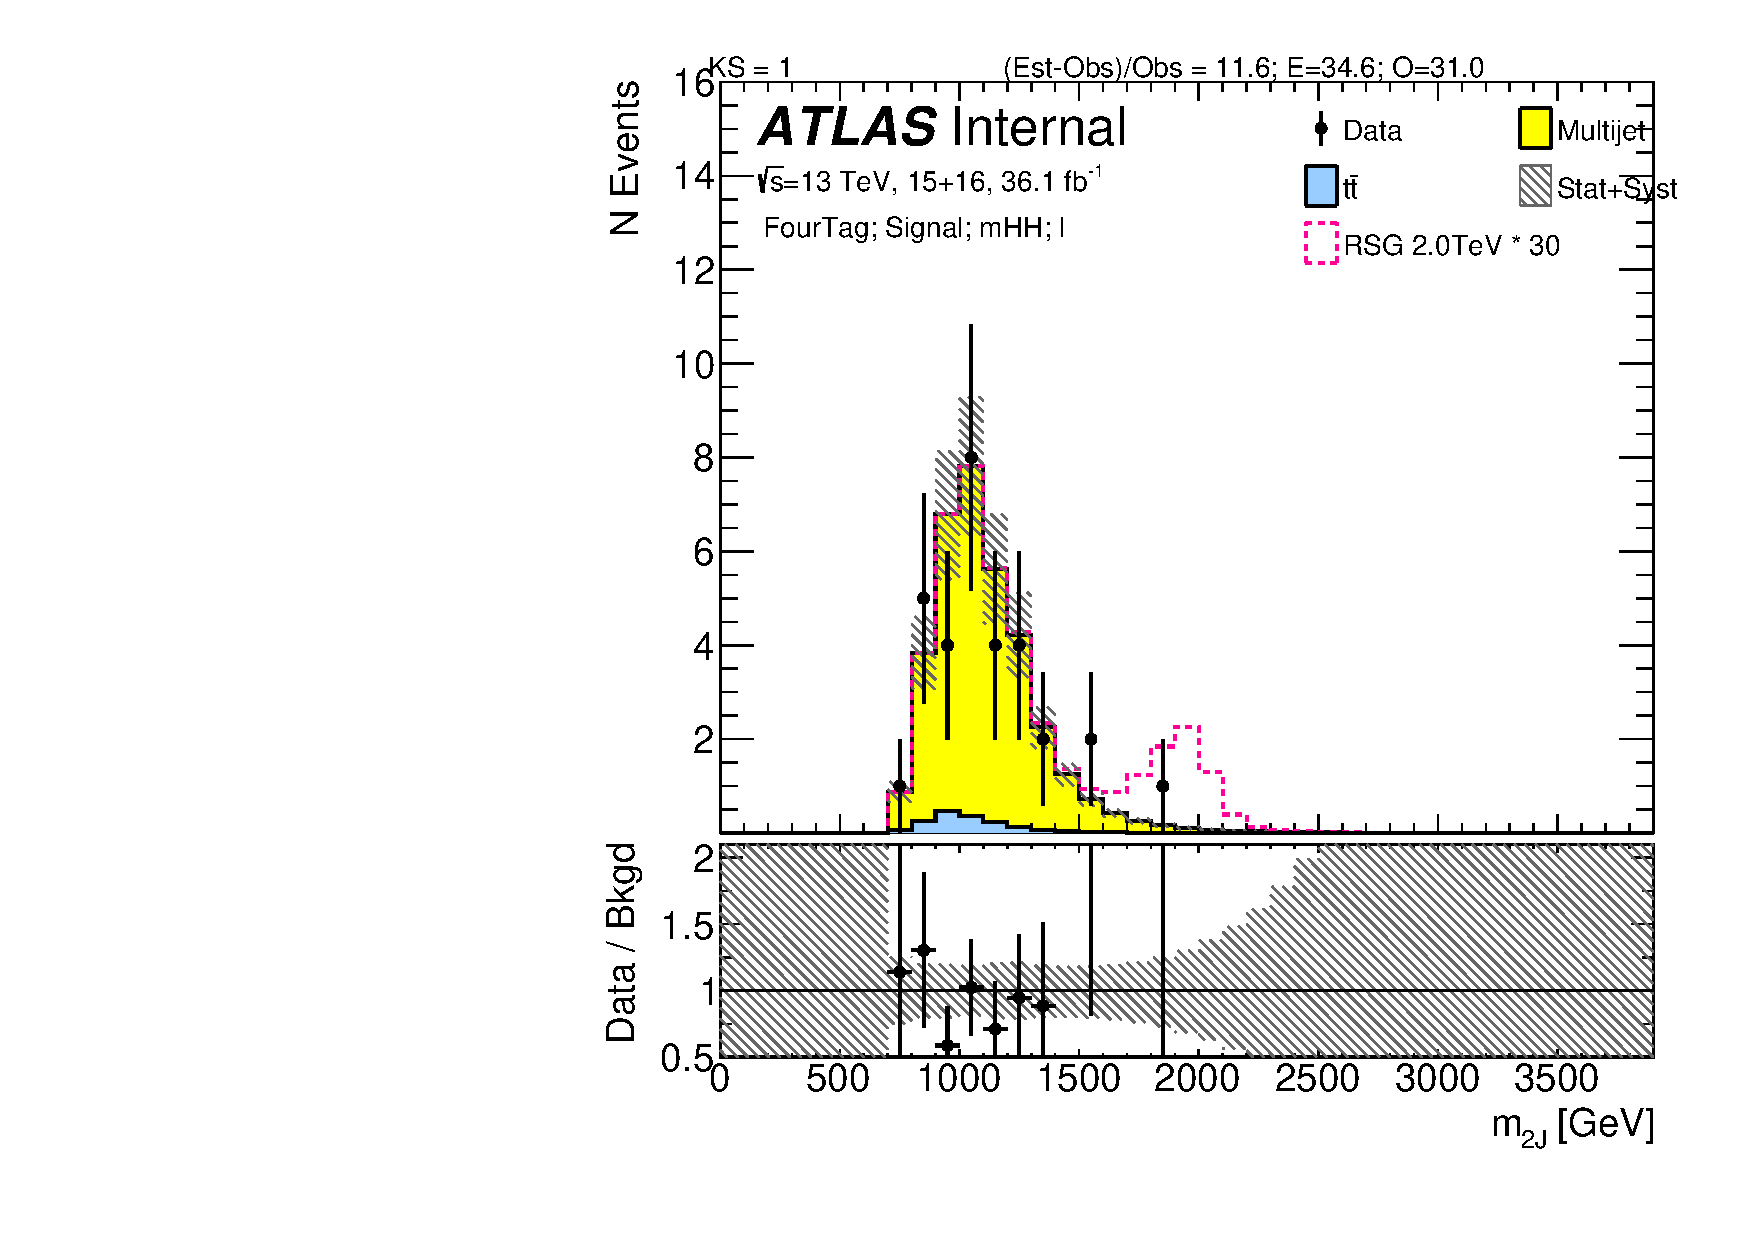
\includegraphics[width=0.31\textwidth,angle=-90]{figures/boosted/Signal_Syst/Moriond_bkg_9_FourTag_Signal_mHH_l.pdf}
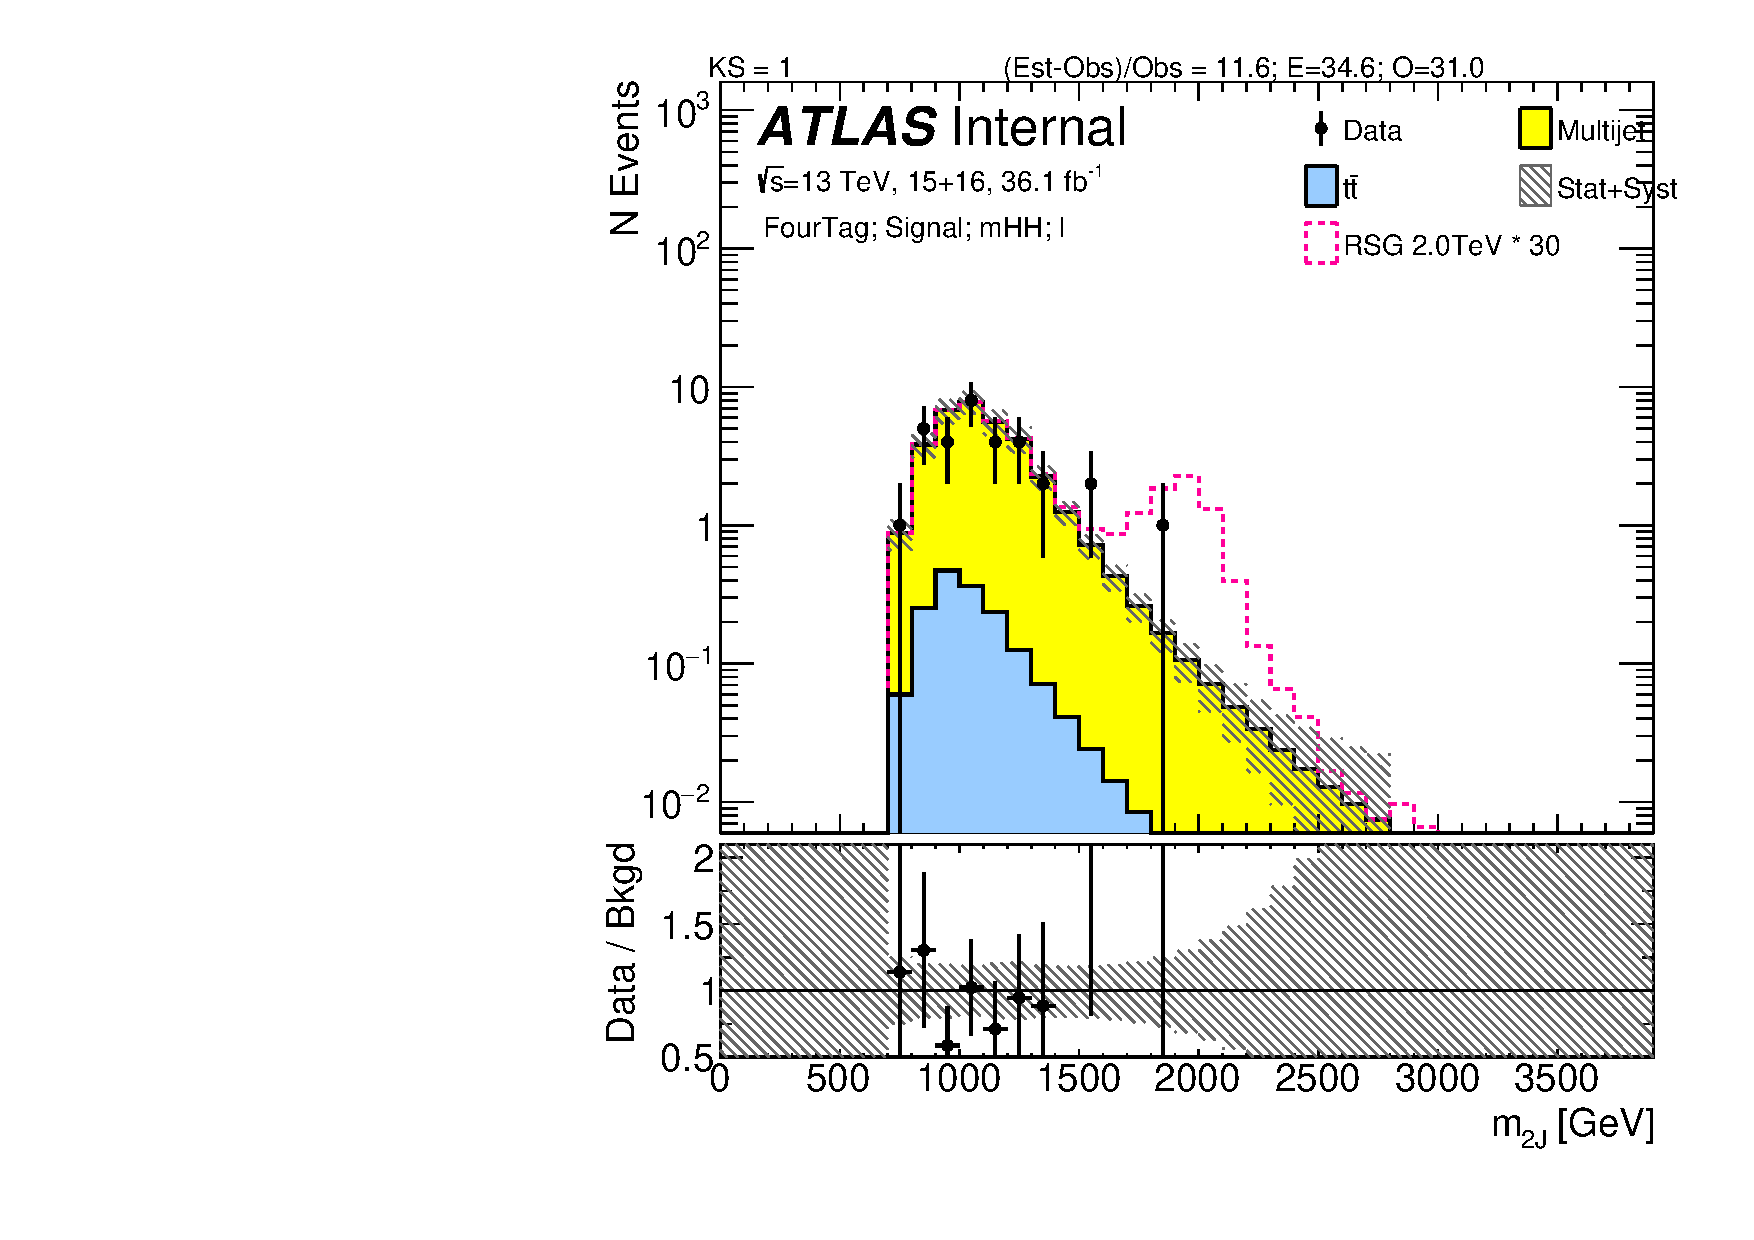
\includegraphics[width=0.31\textwidth,angle=-90]{figures/boosted/Signal_Syst/Moriond_bkg_9_FourTag_Signal_mHH_l_1.pdf}
  \caption{Unscaled dijet mass distribution in the $4b$ Signal Region after unblinding. The left plot is on linear scale and the right plot is on log scale. Stat uncertainty and systematic ucnertainties are shown on the plot.}
  \label{fig:boosted-4b-signal-l}
\end{center}
\end{figure*}

\begin{figure*}[htbp!]
\begin{center}
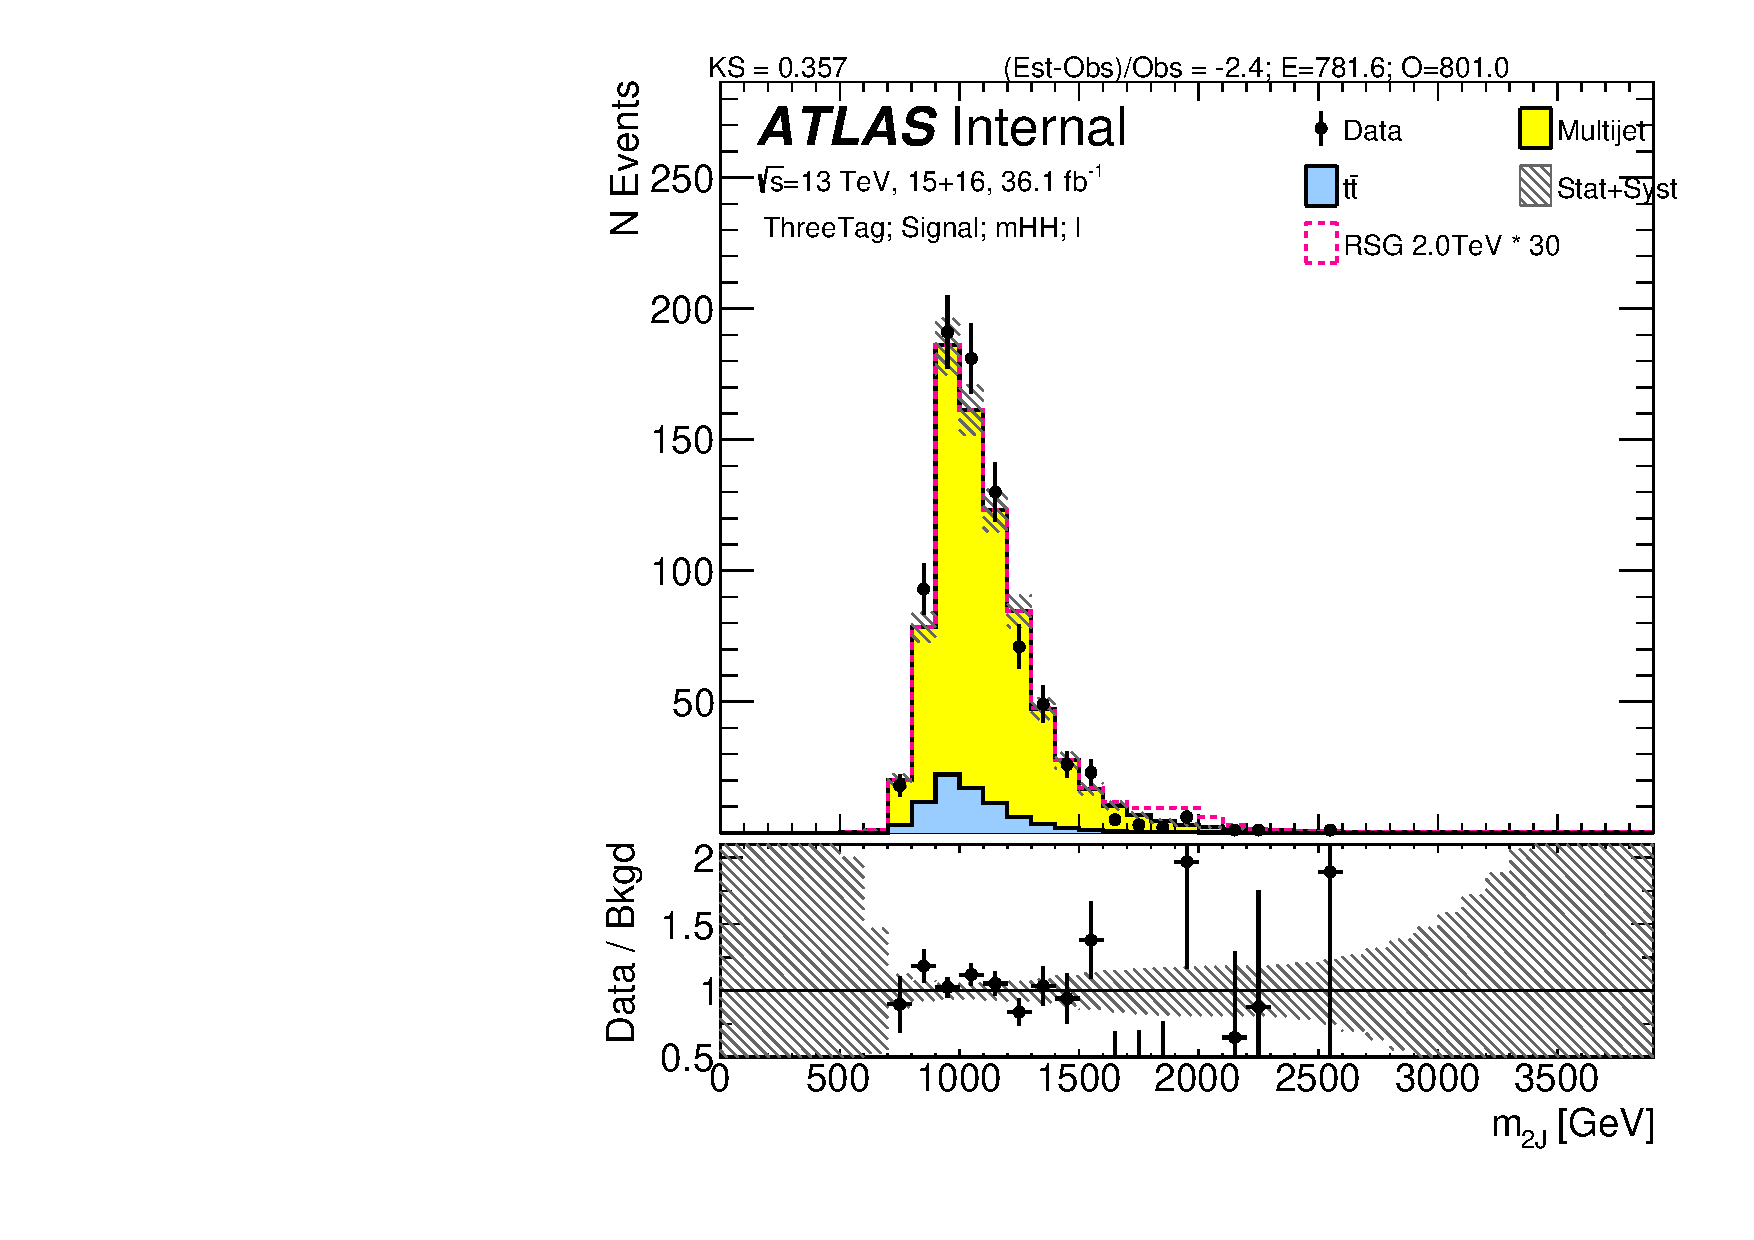
\includegraphics[width=0.31\textwidth,angle=-90]{figures/boosted/Signal_Syst/Moriond_bkg_9_ThreeTag_Signal_mHH_l.pdf}
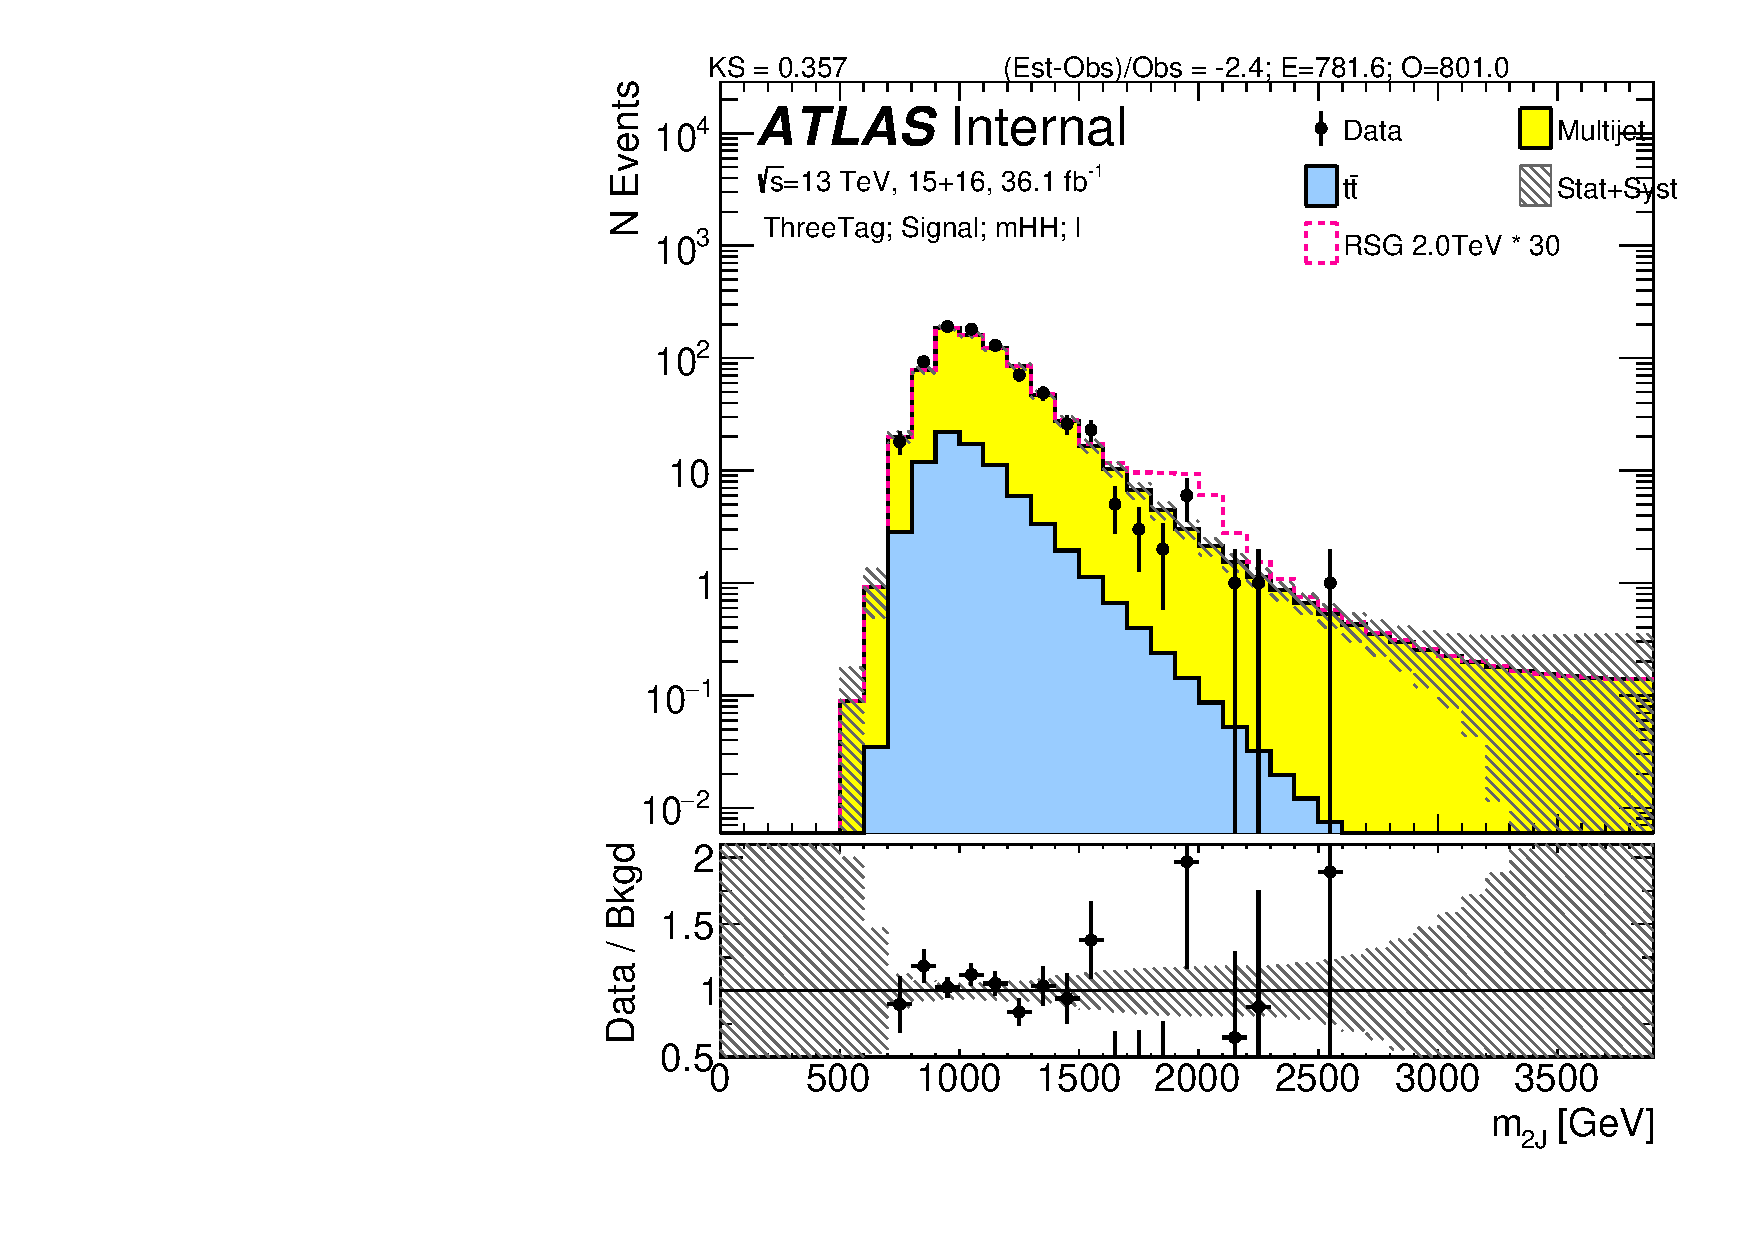
\includegraphics[width=0.31\textwidth,angle=-90]{figures/boosted/Signal_Syst/Moriond_bkg_9_ThreeTag_Signal_mHH_l_1.pdf}  
  \caption{Unscaled dijet mass distribution in the $3b$ Signal Region after unblinding. The left plot is on linear scale and the right plot is on log scale. Stat uncertainty and systematic ucnertainties are shown on the plot.}
  \label{fig:boosted-3b-signal-l}
\end{center}
\end{figure*}

\begin{figure*}[htbp!]
\begin{center}
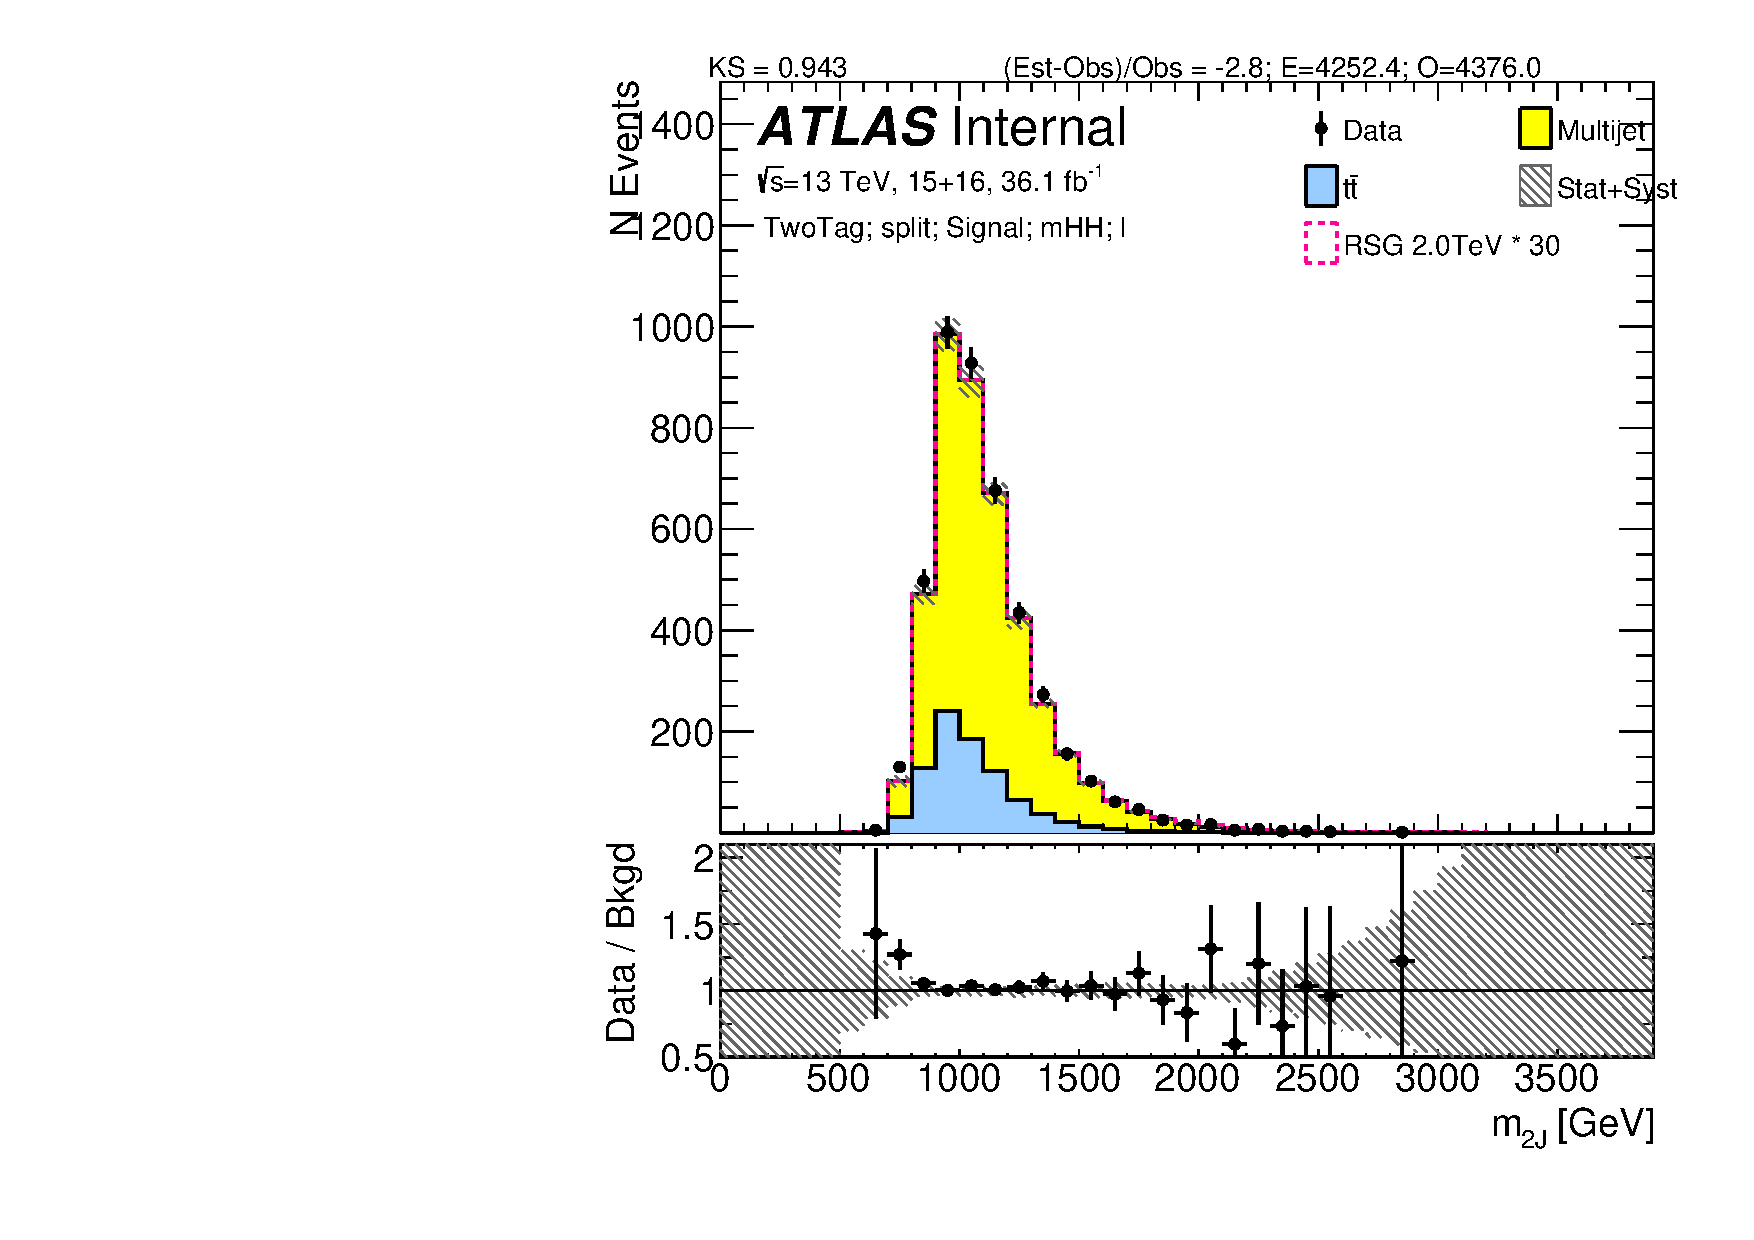
\includegraphics[width=0.31\textwidth,angle=-90]{figures/boosted/Signal_Syst/Moriond_bkg_9_TwoTag_split_Signal_mHH_l.pdf}
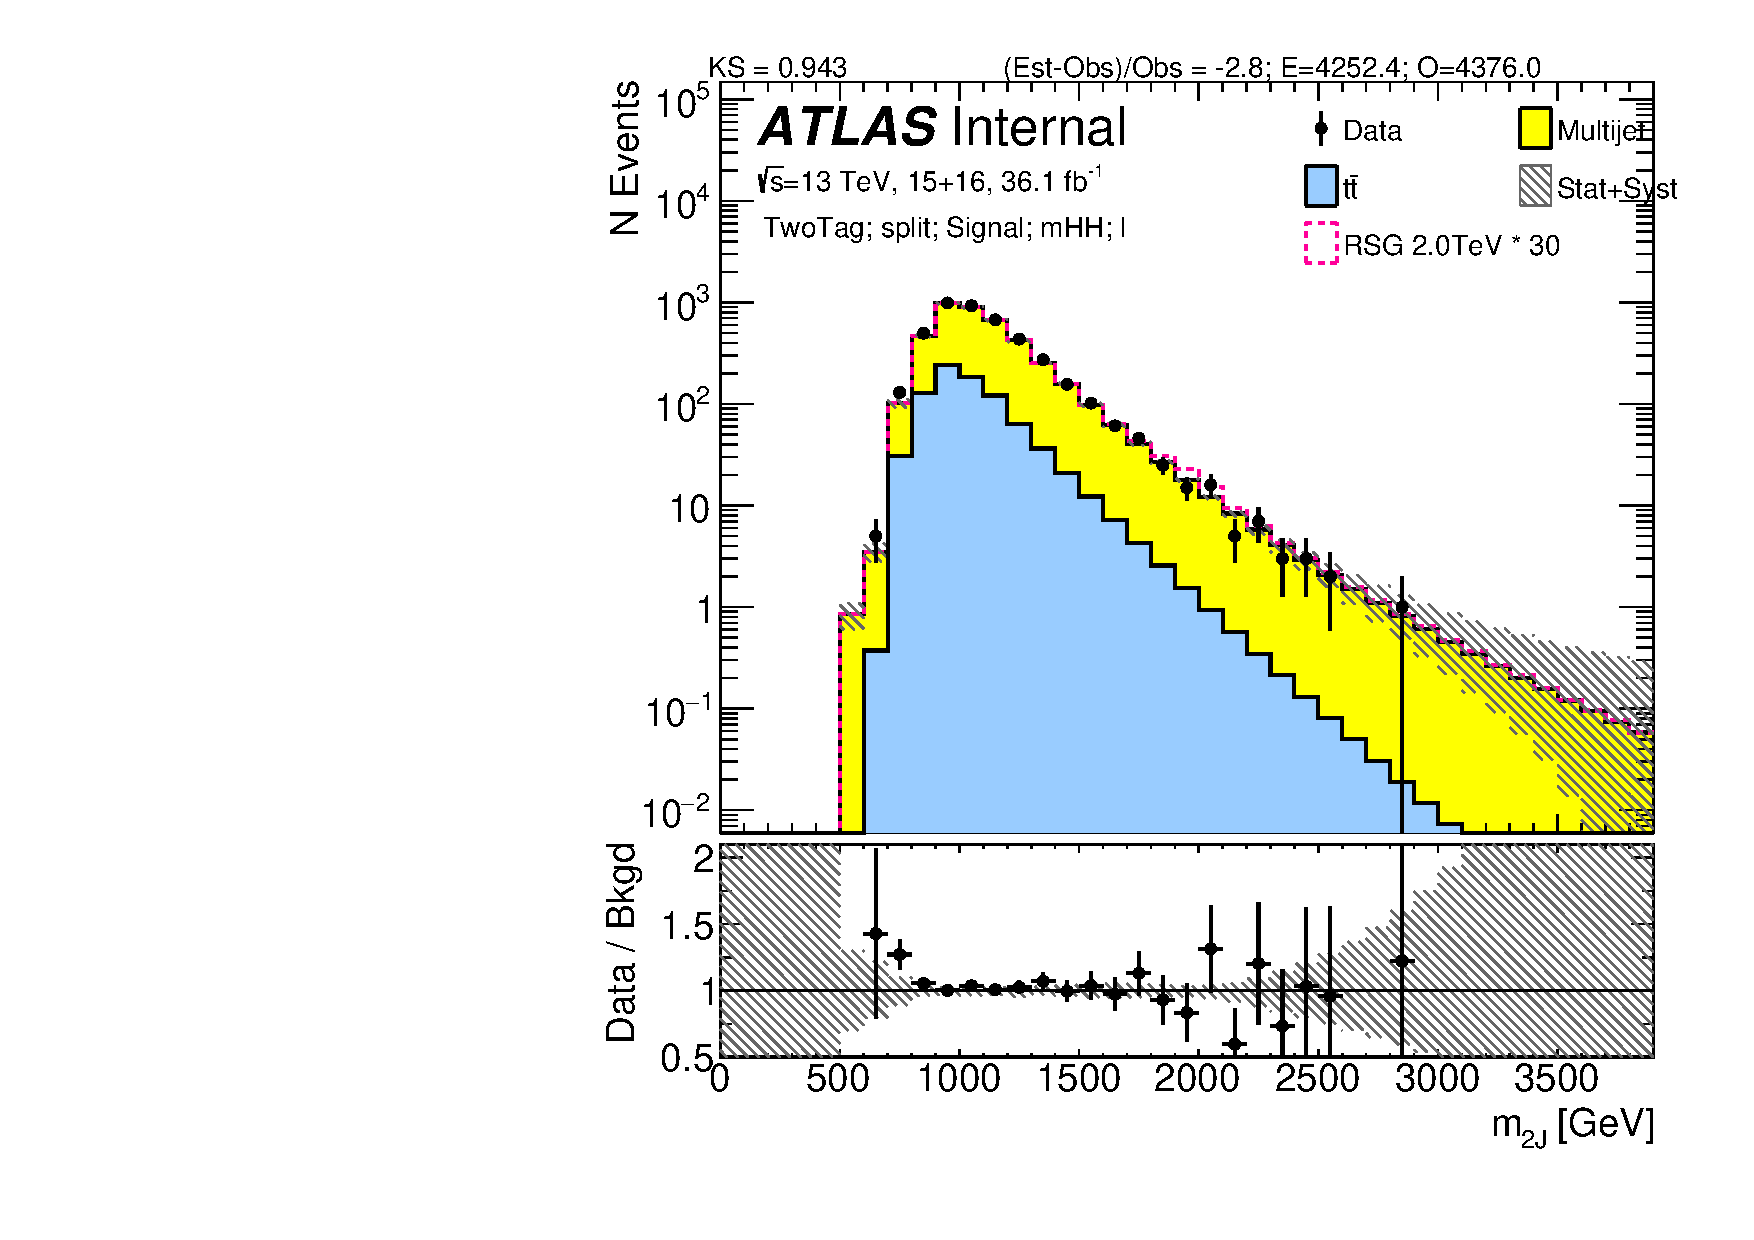
\includegraphics[width=0.31\textwidth,angle=-90]{figures/boosted/Signal_Syst/Moriond_bkg_9_TwoTag_split_Signal_mHH_l_1.pdf}  
  \caption{Unscaled dijet mass distribution in the $2bs$ Signal Region after unblinding. The left plot is on linear scale and the right plot is on log scale. Stat uncertainty and systematic ucnertainties are shown on the plot.}
  \label{fig:boosted-2b-signal-l}
\end{center}
\end{figure*}

\begin{figure*}[htbp!]
\begin{center}
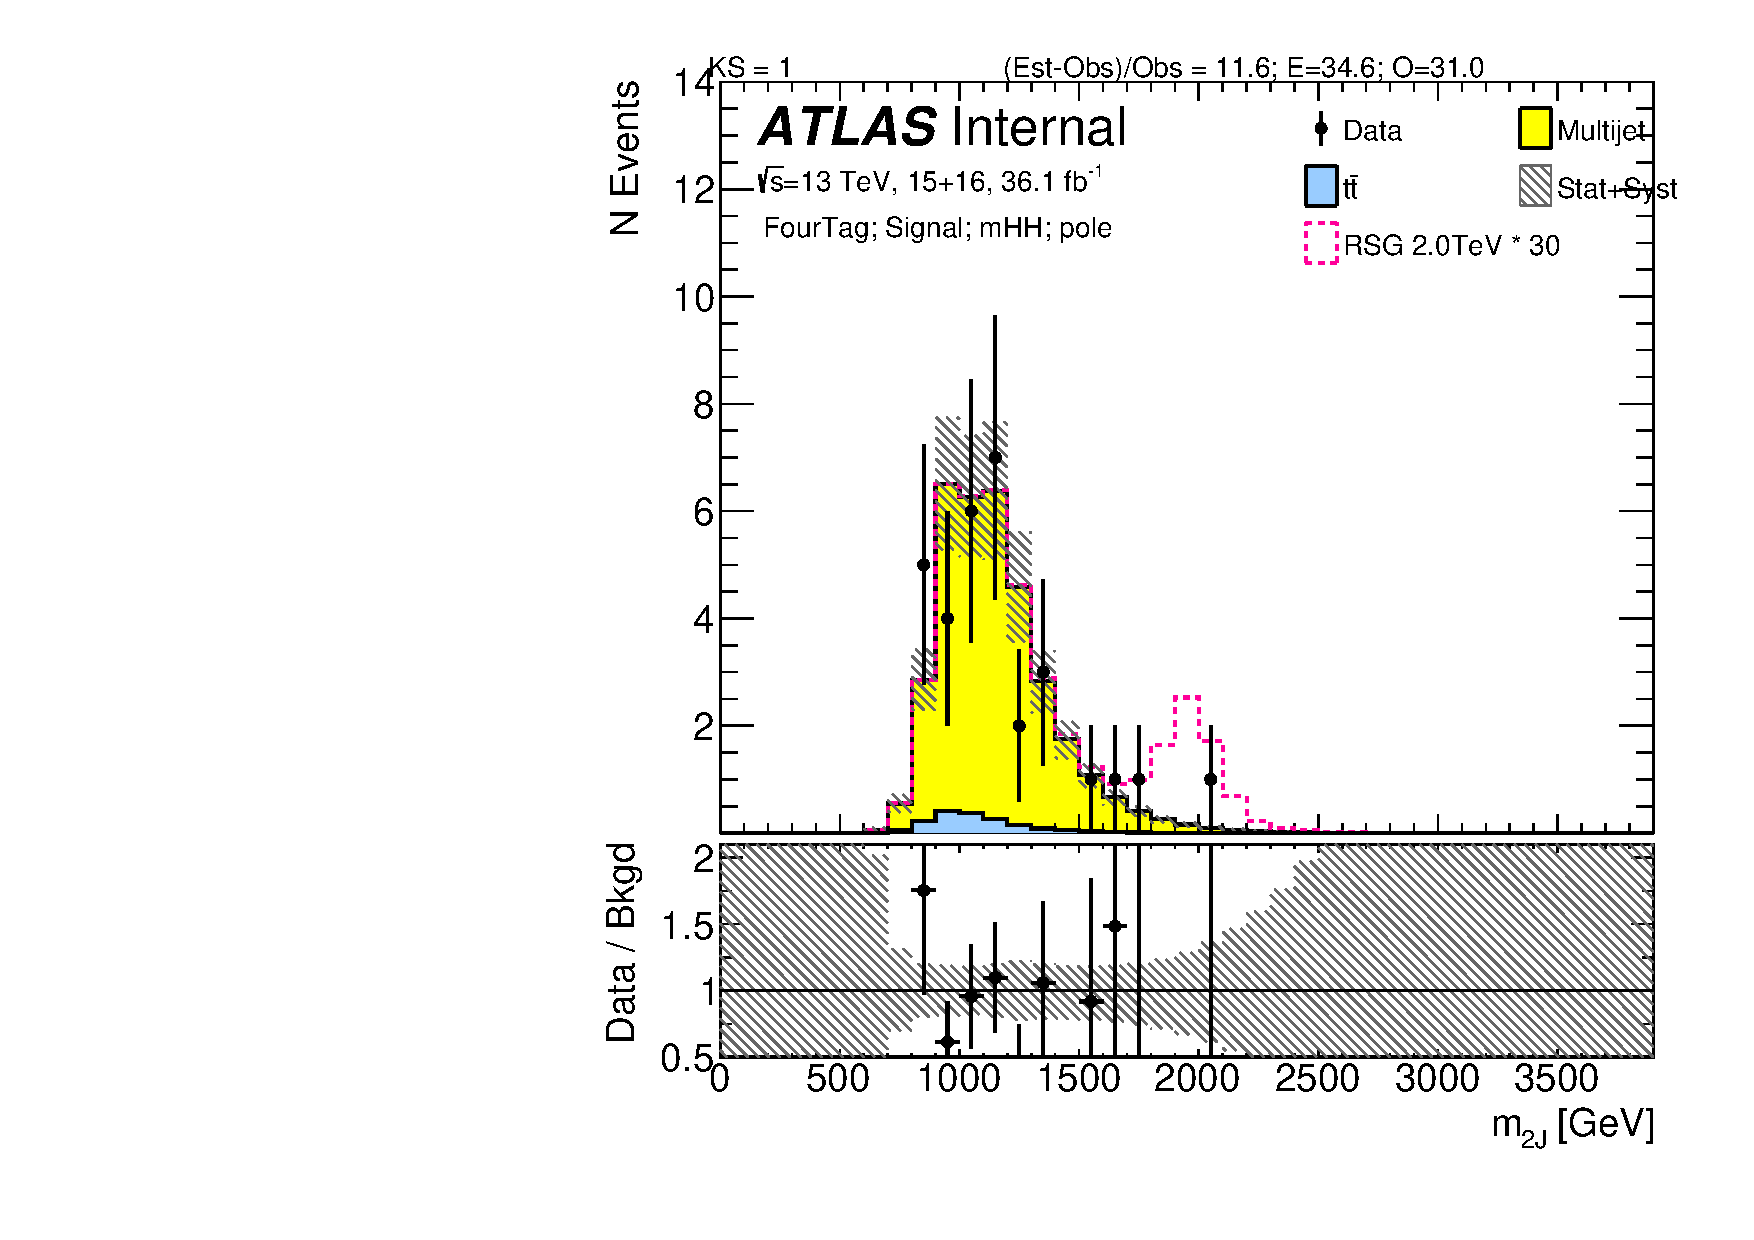
\includegraphics[width=0.31\textwidth,angle=-90]{figures/boosted/Signal_Syst/Moriond_bkg_9_FourTag_Signal_mHH_pole.pdf}
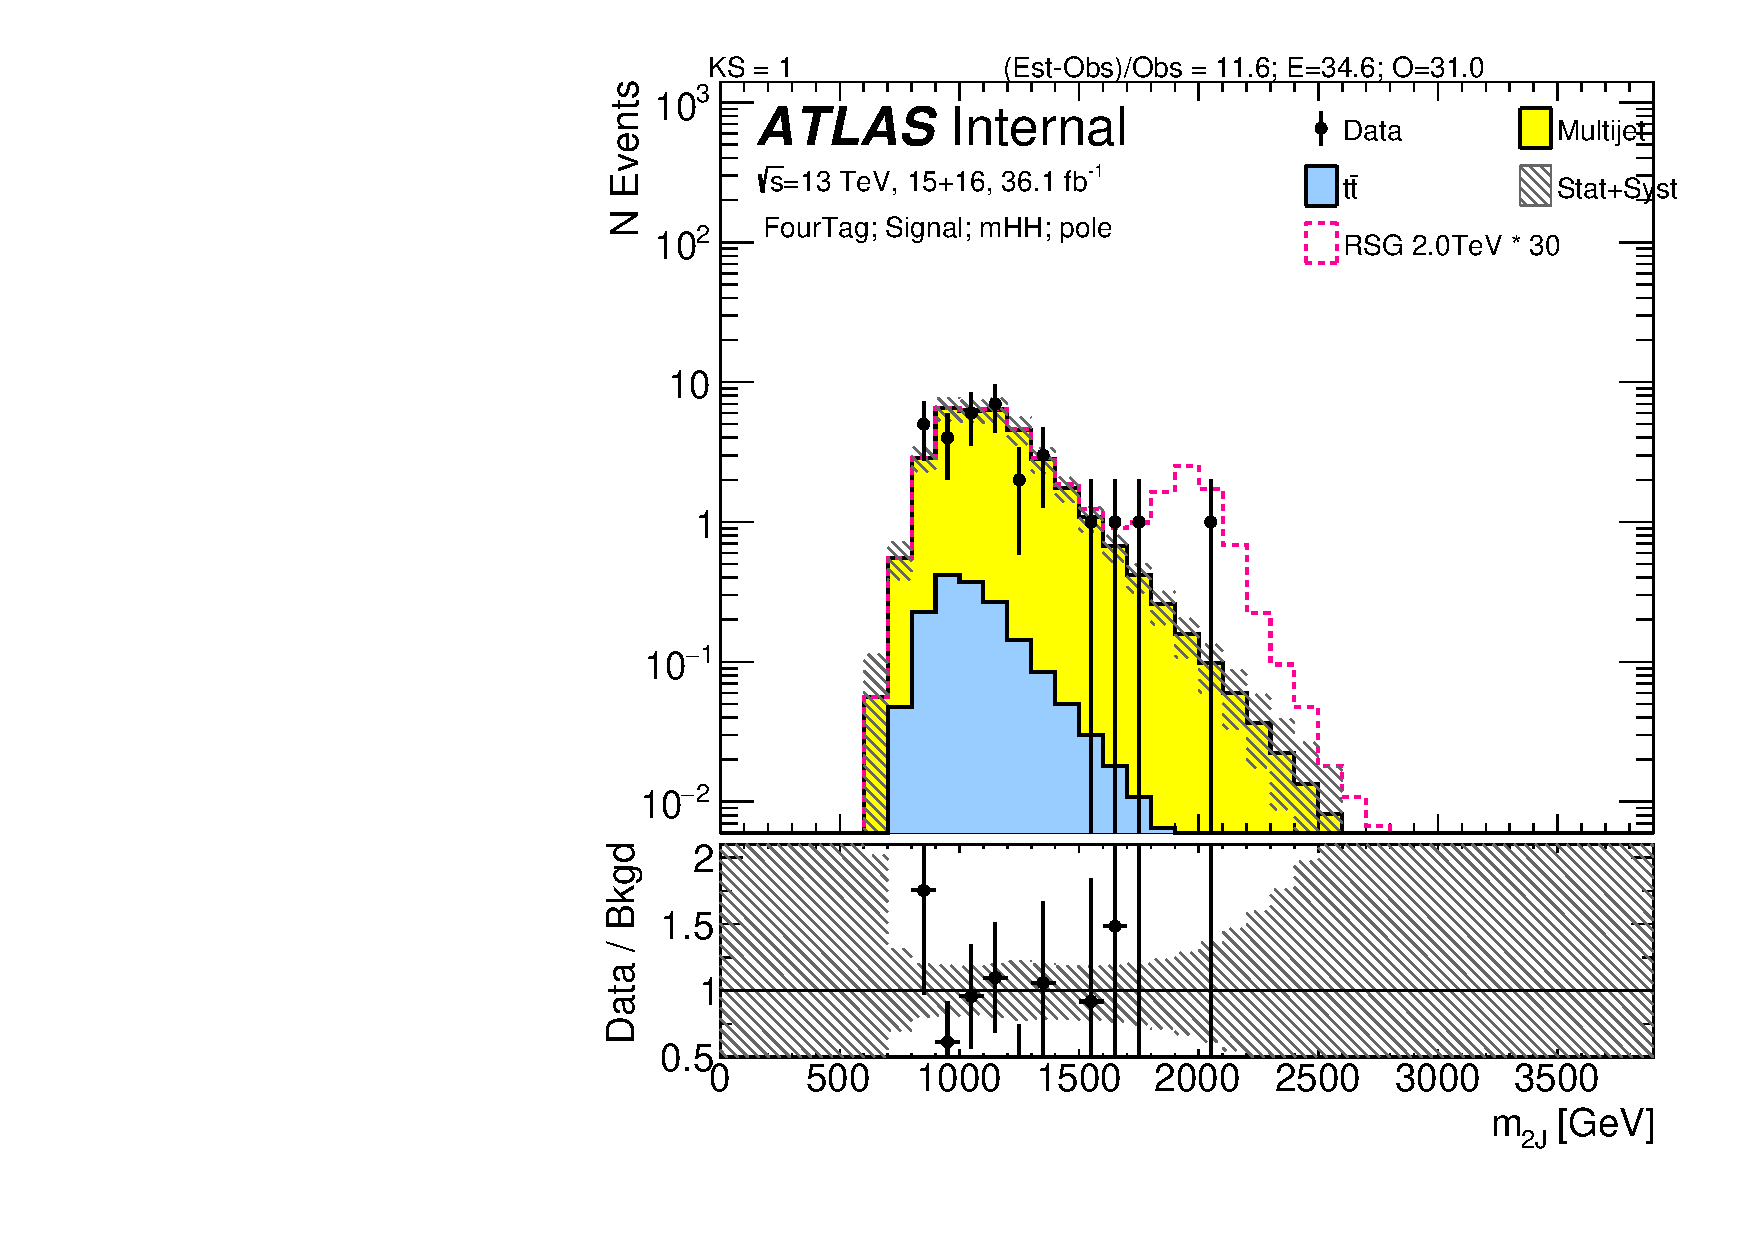
\includegraphics[width=0.31\textwidth,angle=-90]{figures/boosted/Signal_Syst/Moriond_bkg_9_FourTag_Signal_mHH_pole_1.pdf}
  \caption{Scaled dijet mass distribution in the $4b$ Signal Region after unblinding. The left plot is on linear scale and the right plot is on log scale. Stat uncertainty and systematic ucnertainties are shown on the plot.}
  \label{fig:boosted-4b-signal-pole}
\end{center}
\end{figure*}

\begin{figure*}[htbp!]
\begin{center}
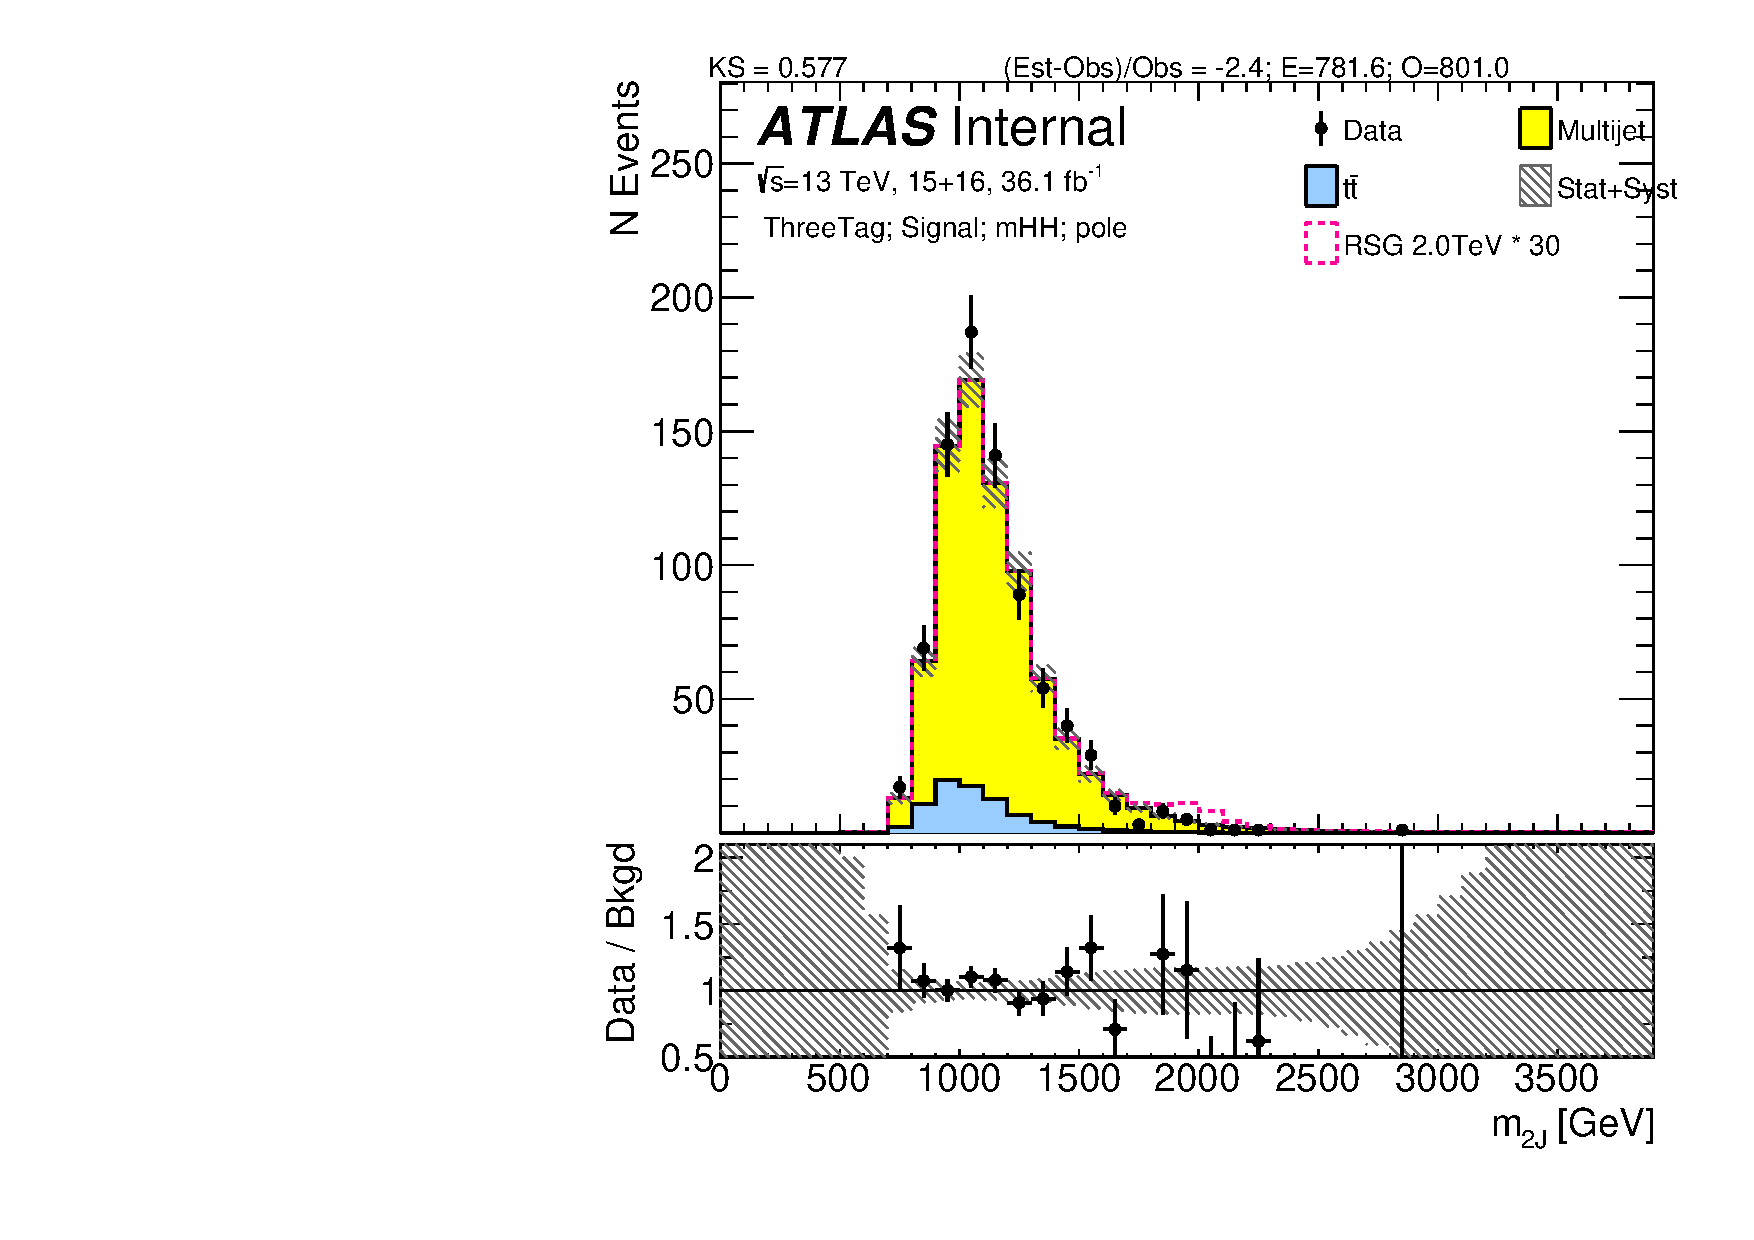
\includegraphics[width=0.31\textwidth,angle=-90]{figures/boosted/Signal_Syst/Moriond_bkg_9_ThreeTag_Signal_mHH_pole.pdf}
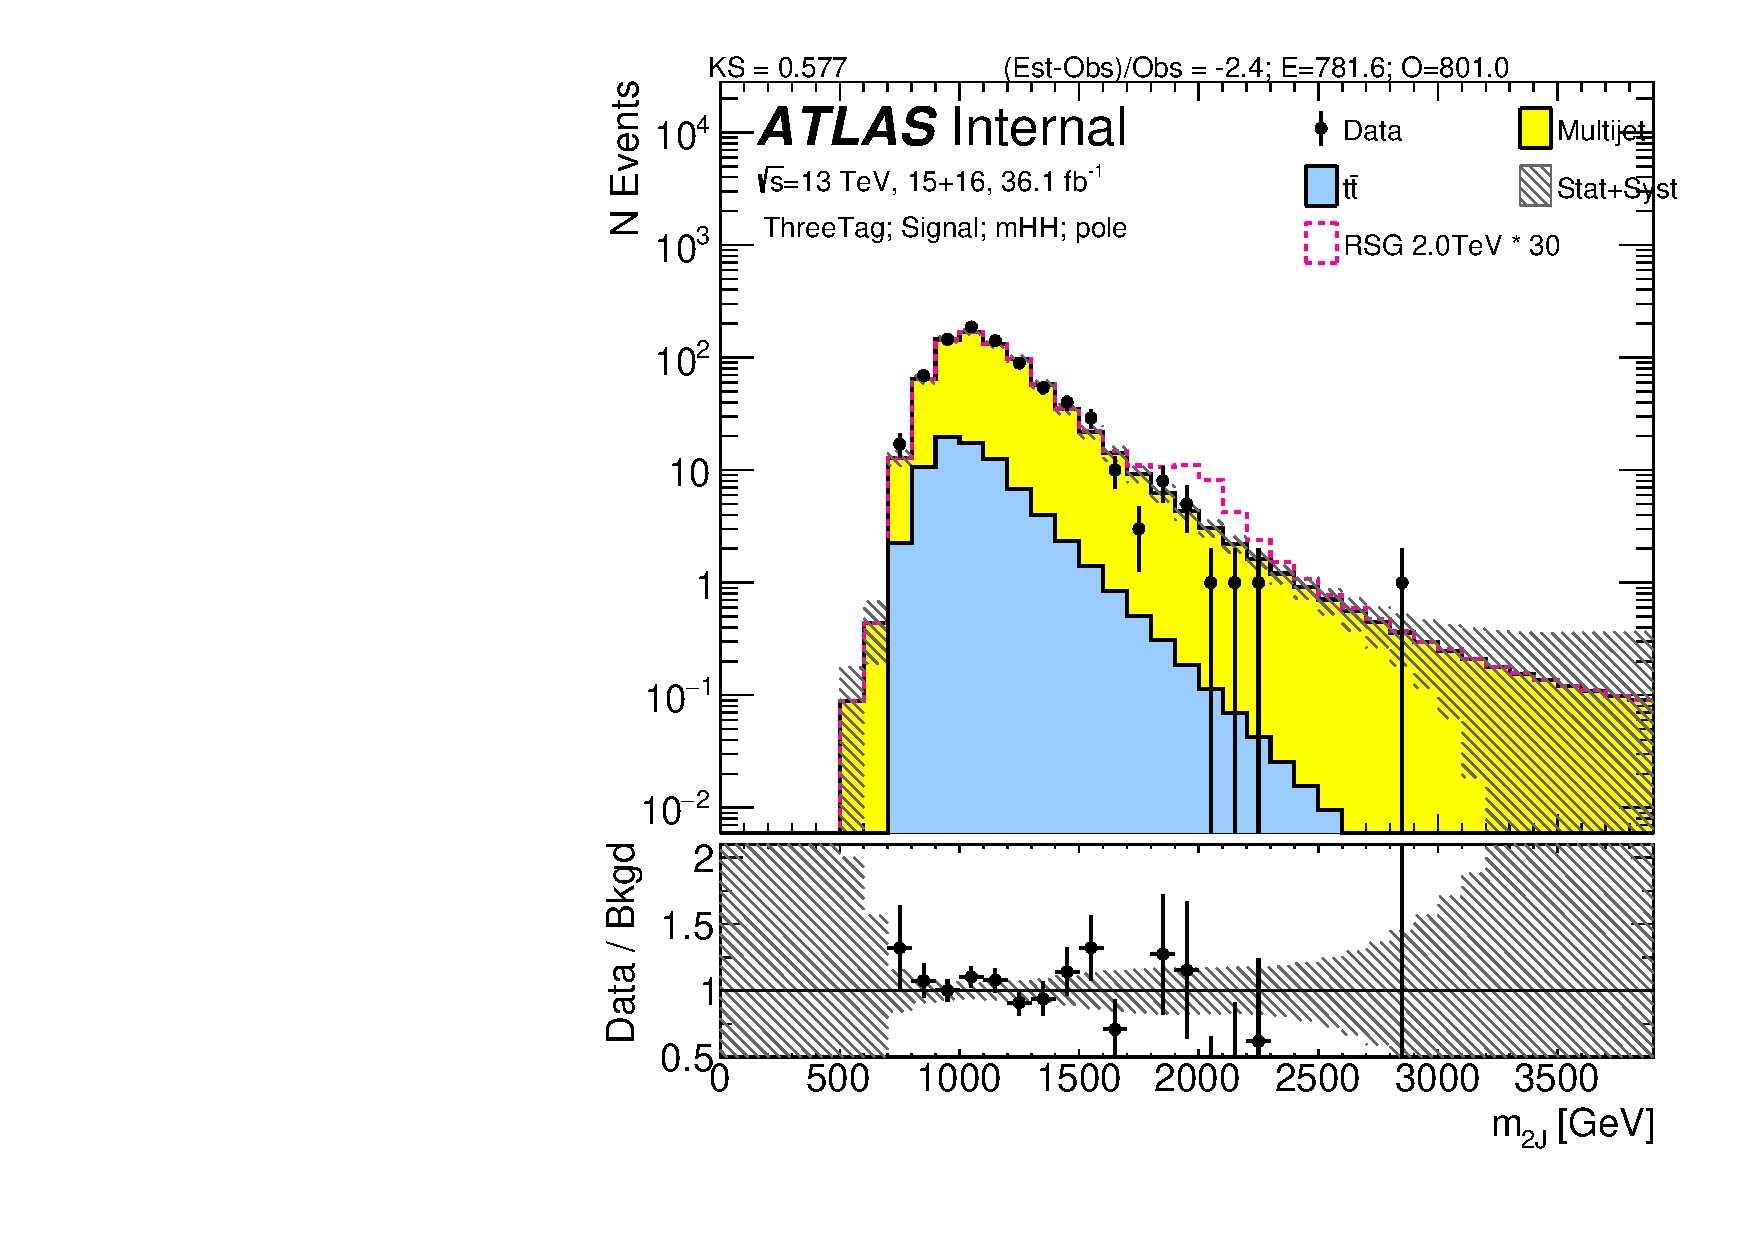
\includegraphics[width=0.31\textwidth,angle=-90]{figures/boosted/Signal_Syst/Moriond_bkg_9_ThreeTag_Signal_mHH_pole_1.pdf}  
  \caption{Scaled dijet mass distribution in the $3b$ Signal Region after unblinding. The left plot is on linear scale and the right plot is on log scale. Stat uncertainty and systematic ucnertainties are shown on the plot.}
  \label{fig:boosted-3b-signal-pole}
\end{center}
\end{figure*}

\begin{figure*}[htbp!]
\begin{center}
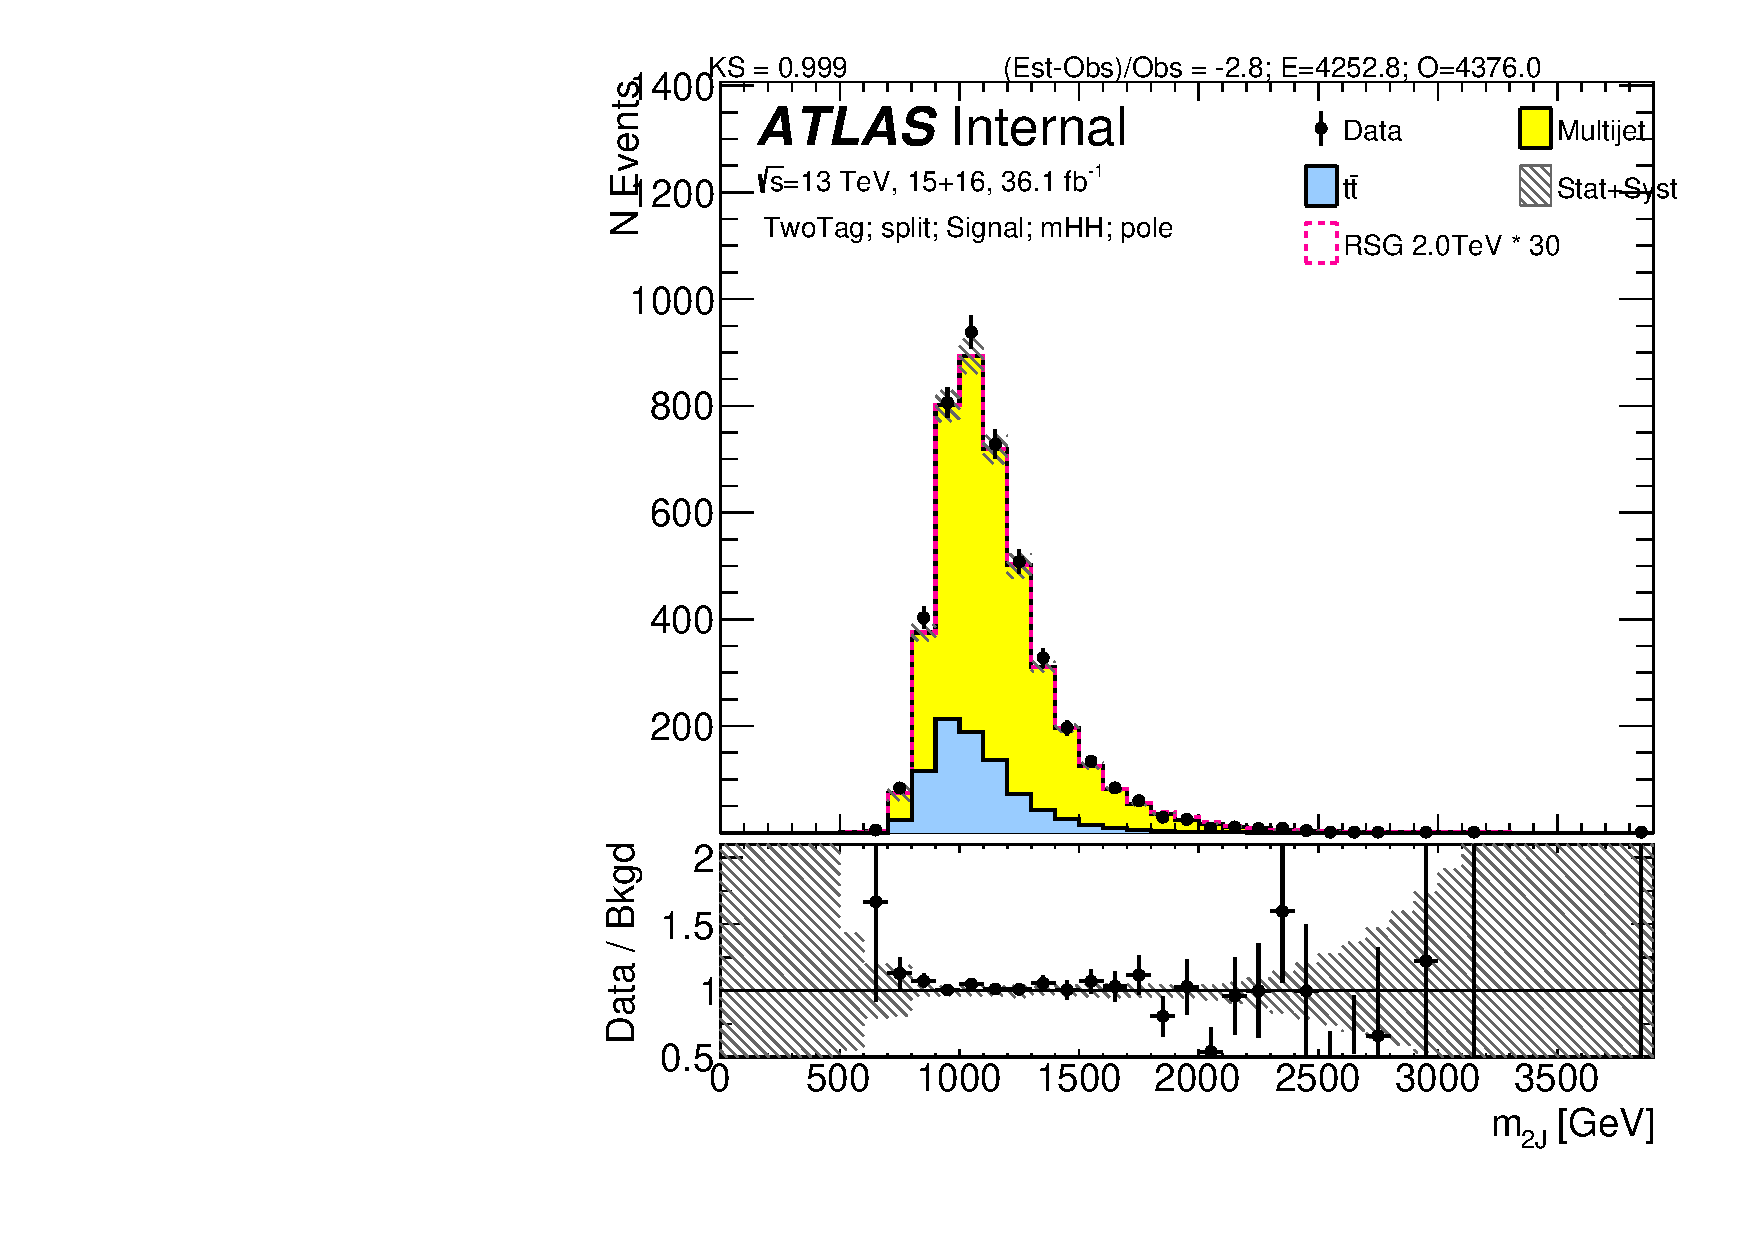
\includegraphics[width=0.31\textwidth,angle=-90]{figures/boosted/Signal_Syst/Moriond_bkg_9_TwoTag_split_Signal_mHH_pole.pdf}
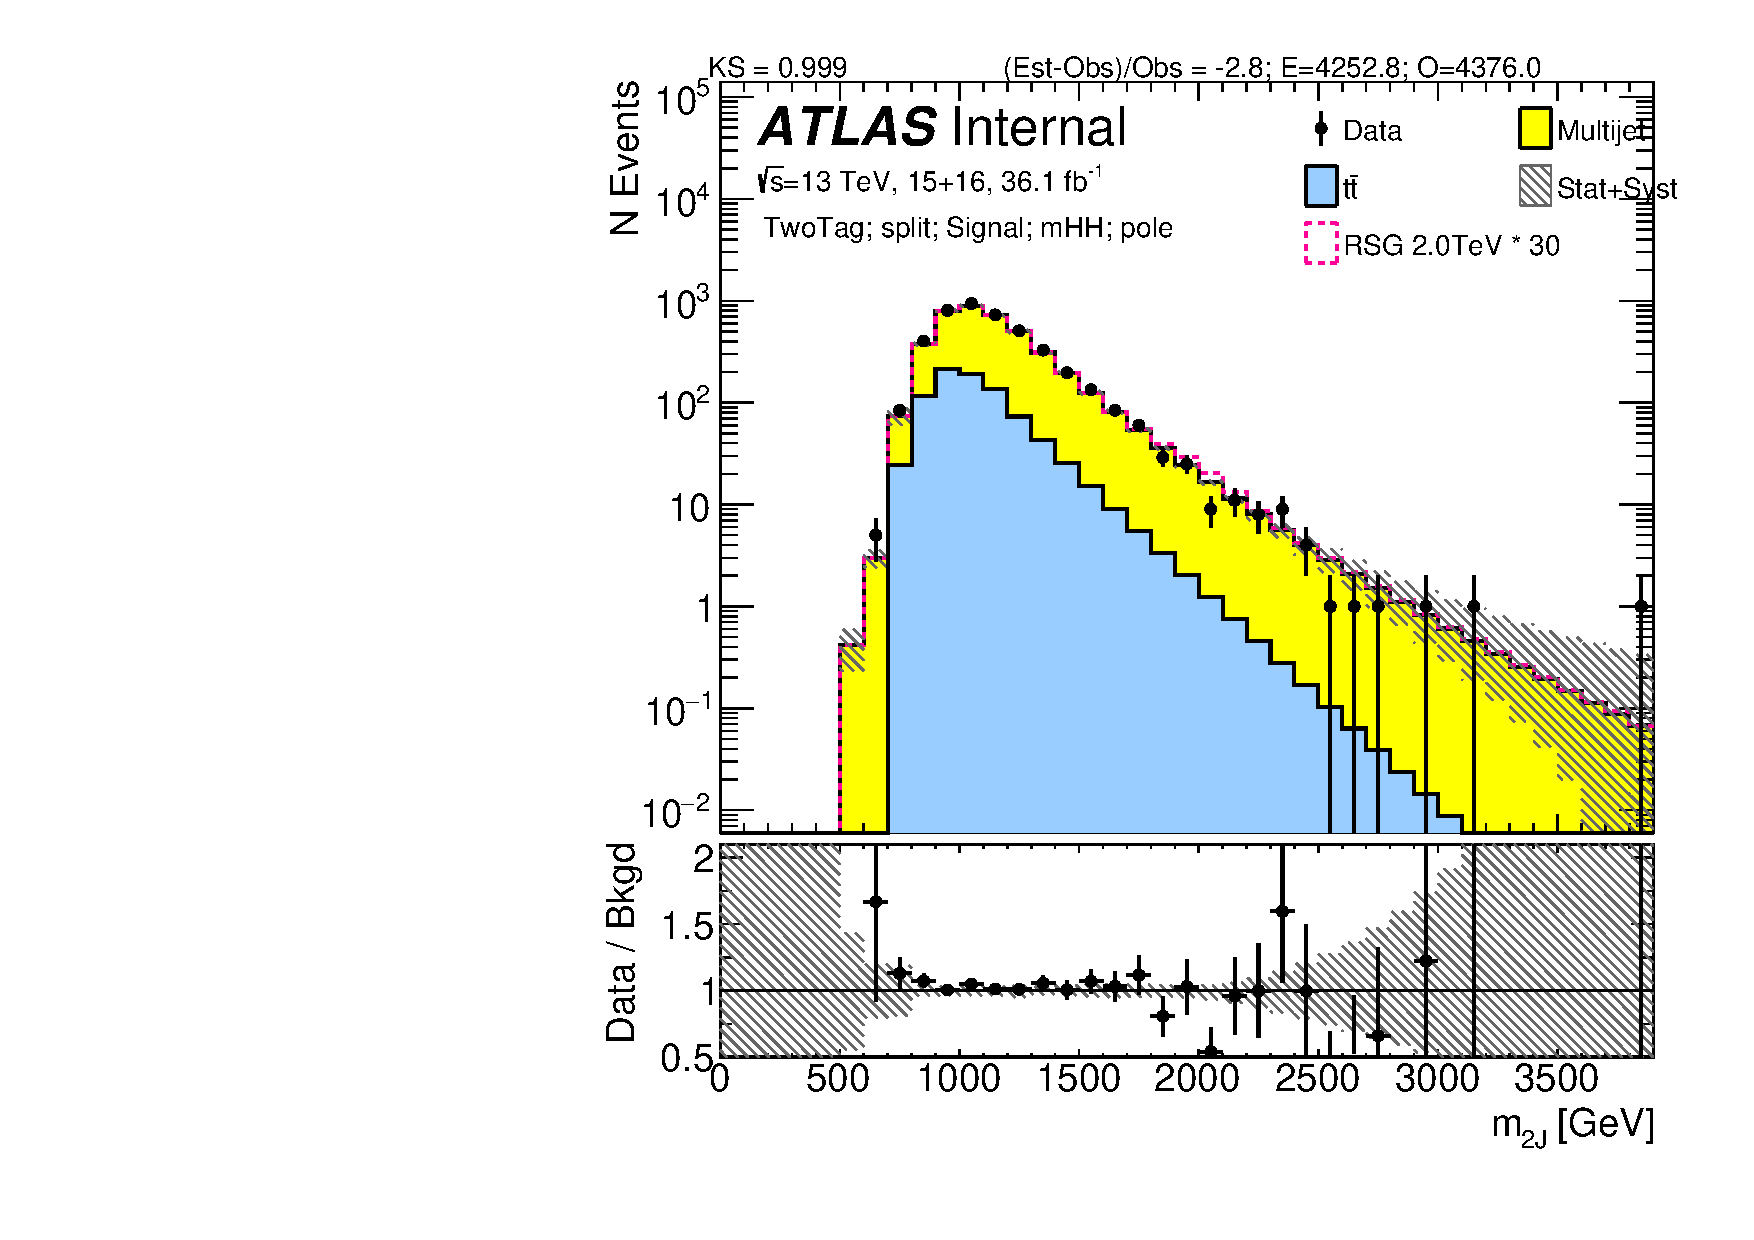
\includegraphics[width=0.31\textwidth,angle=-90]{figures/boosted/Signal_Syst/Moriond_bkg_9_TwoTag_split_Signal_mHH_pole_1.pdf}  
  \caption{Scaled dijet mass distribution in the $2bs$ Signal Region after unblinding. The left plot is on linear scale and the right plot is on log scale. Stat uncertainty and systematic ucnertainties are shown on the plot.}
  \label{fig:boosted-2b-signal-pole}
\end{center}
\end{figure*}

\paragraph{}
Here the results are displayed for the mass range that includes the boosted categories (ie. 800 GeV and above).  In the range 800-1400 GeV the boosted categories are combined with the resolved categories. The full mass range results are collected in the resolved note.

\paragraph{}
A search for statistically significant deviation from the background model hypothesis is performed following the procedure described in Sec.\,\ref{sec-search-procedure}, computing the local $p_0$ value using the asymptotic approximation.

\paragraph{}
The background model is found to describe the data and no significant excess is observed. The smallest local $p_0=0.175$ (1$\sigma$) is found at 1100 GeV when fitting with the narrow scalar model. The local $p_0$ values for the three signal models as a function of the resonance mass are shown in Fig.~\ref{fig:localp0}.

\begin{figure*}[htbp!]
\begin{center}
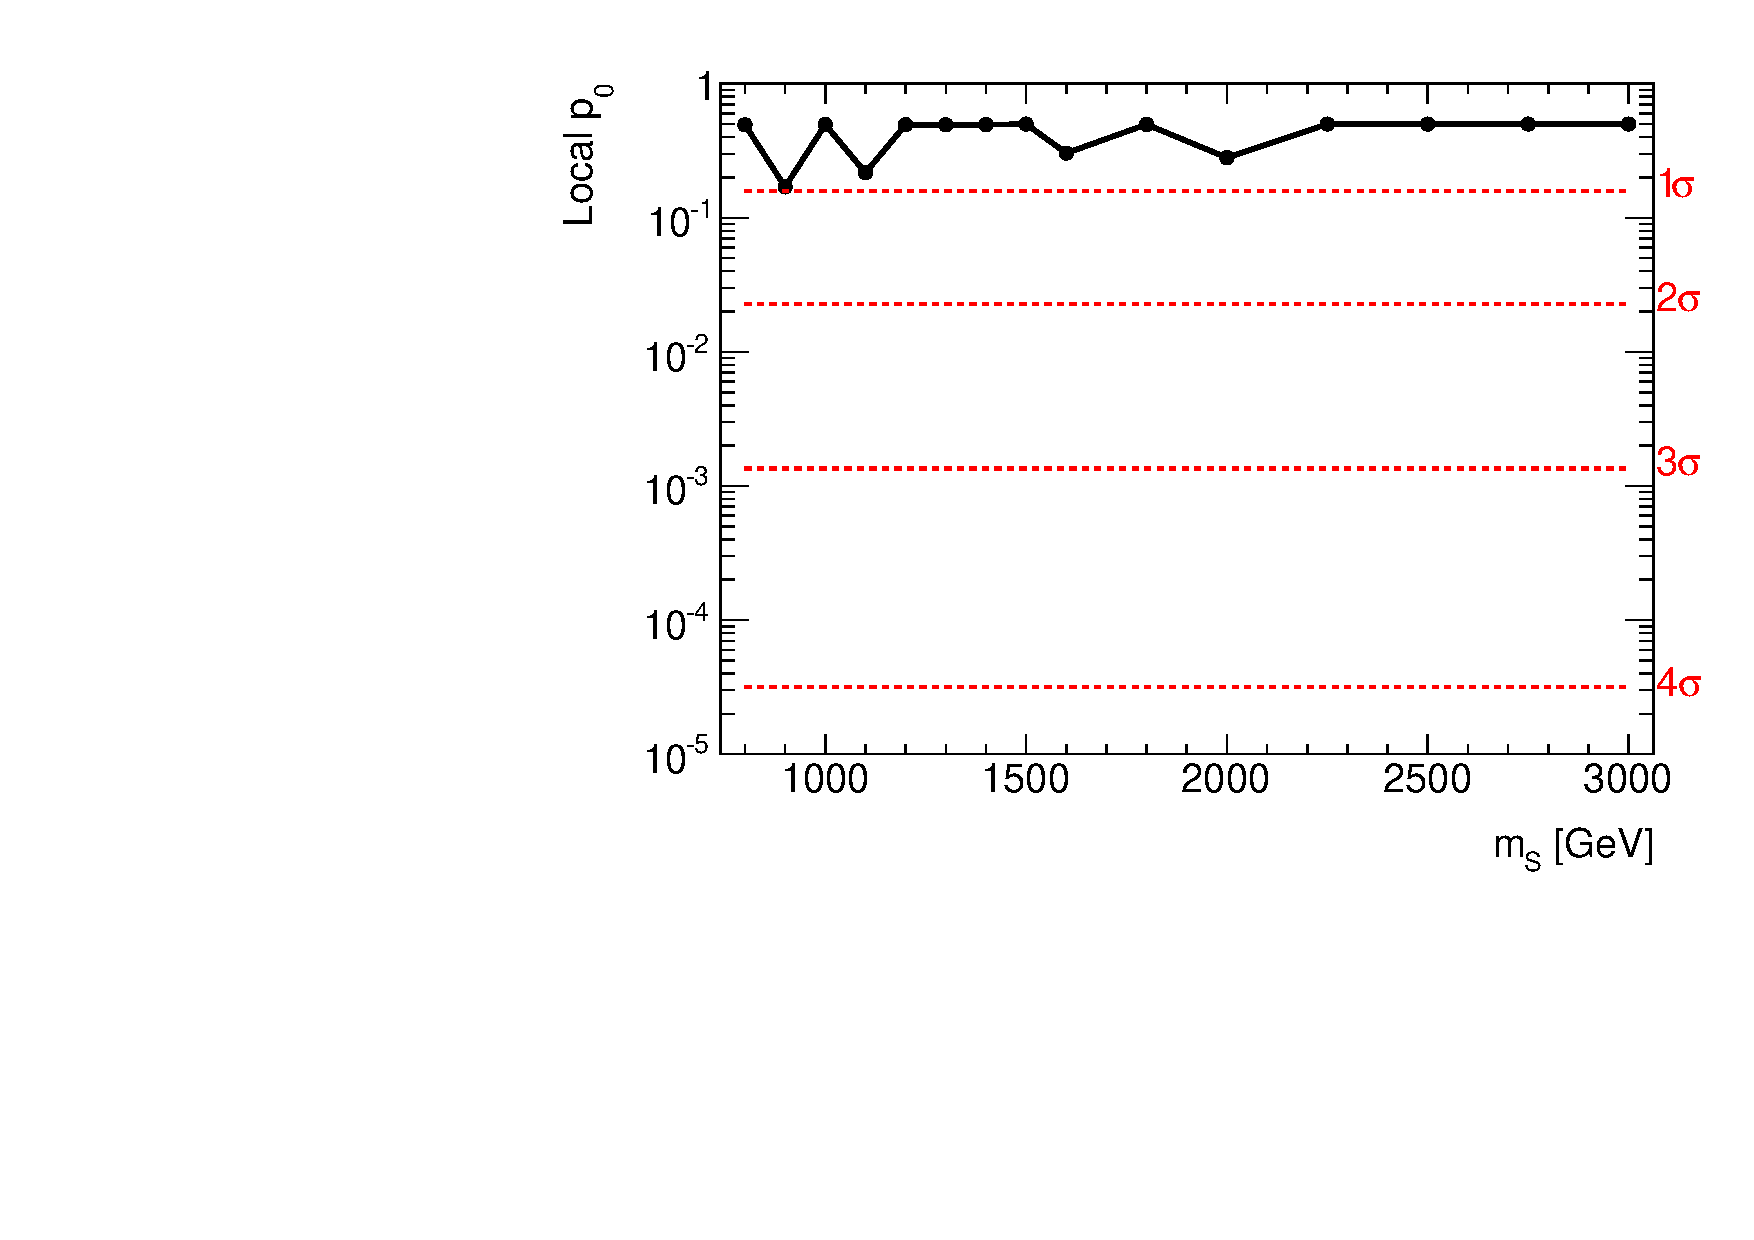
\includegraphics[width=0.21\textwidth,angle=-90]{figures/boosted/results/p0_s_allmasses_boosted.pdf}
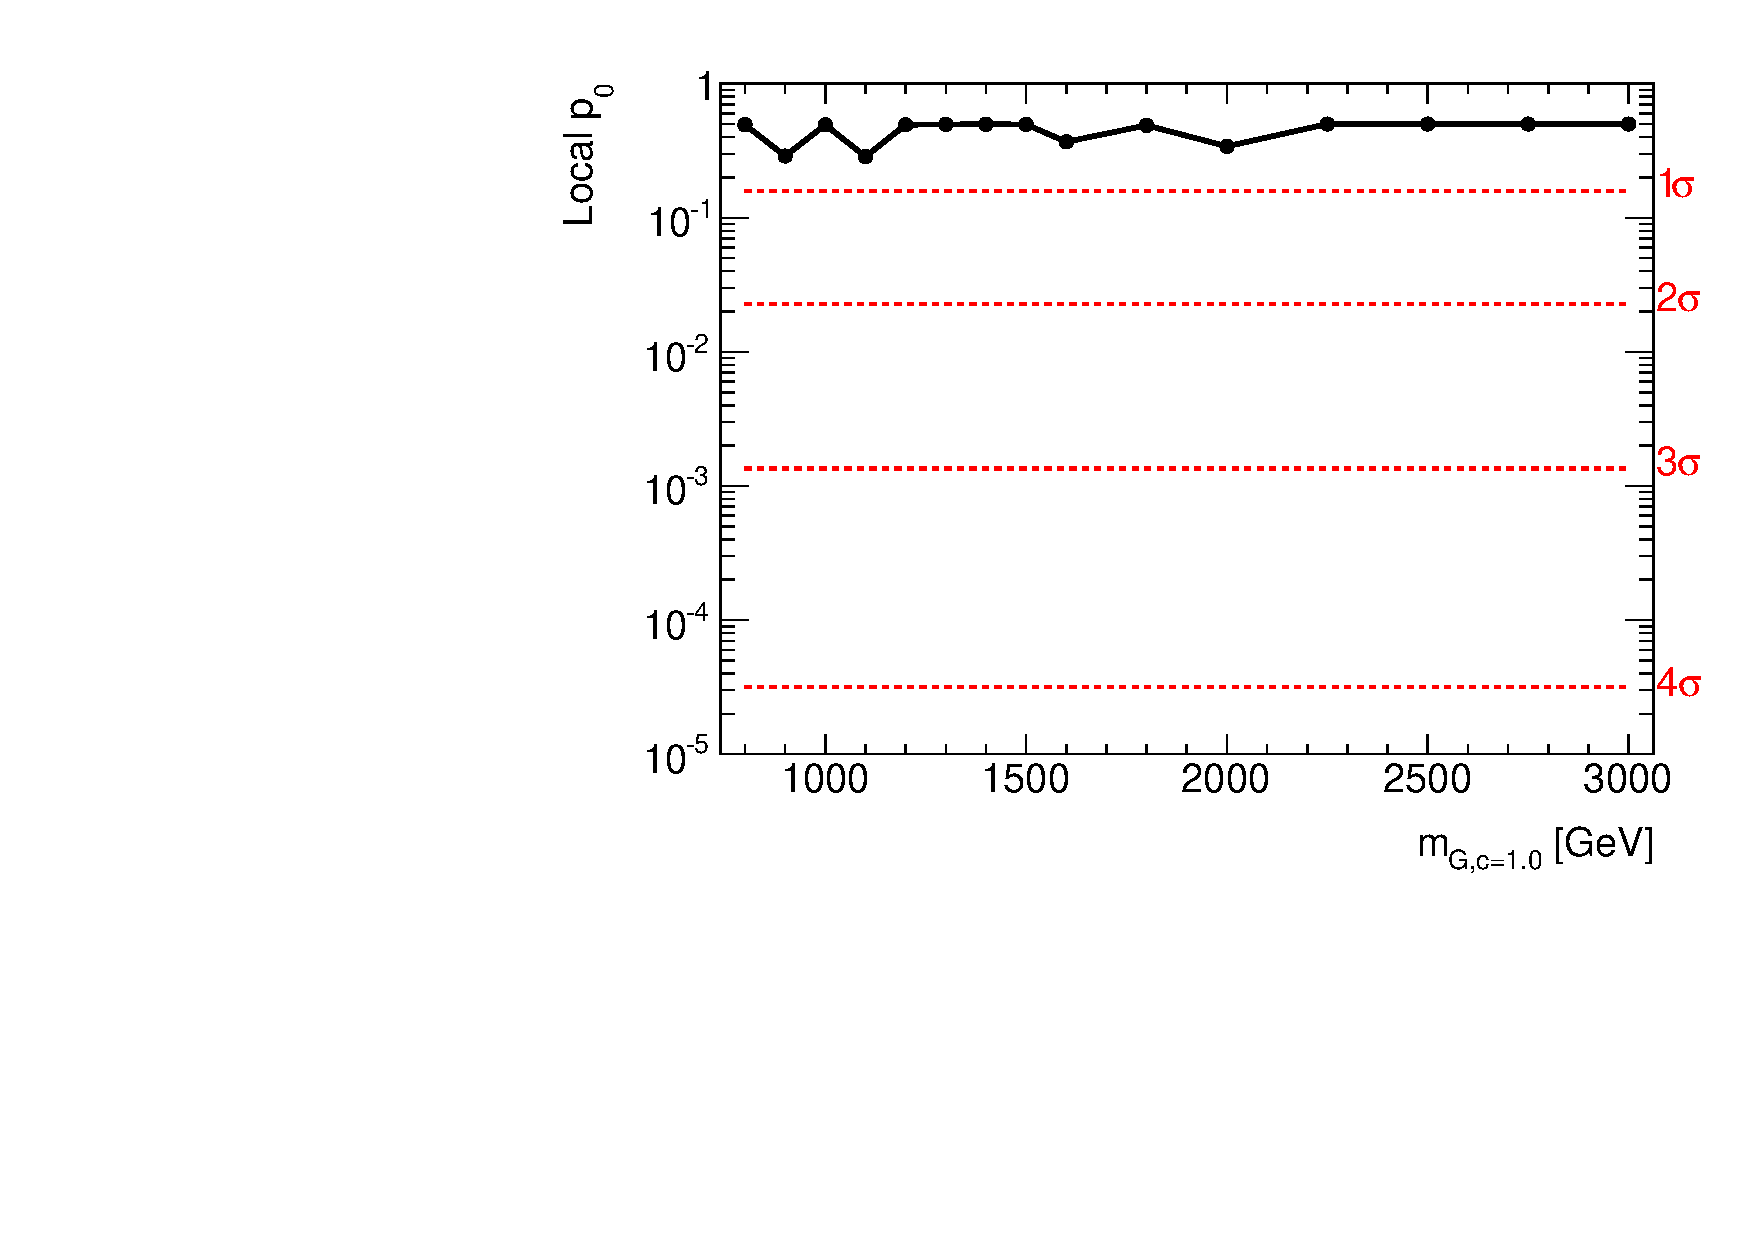
\includegraphics[width=0.21\textwidth,angle=-90]{figures/boosted/results/p0_g10_allmasses_boosted.pdf}
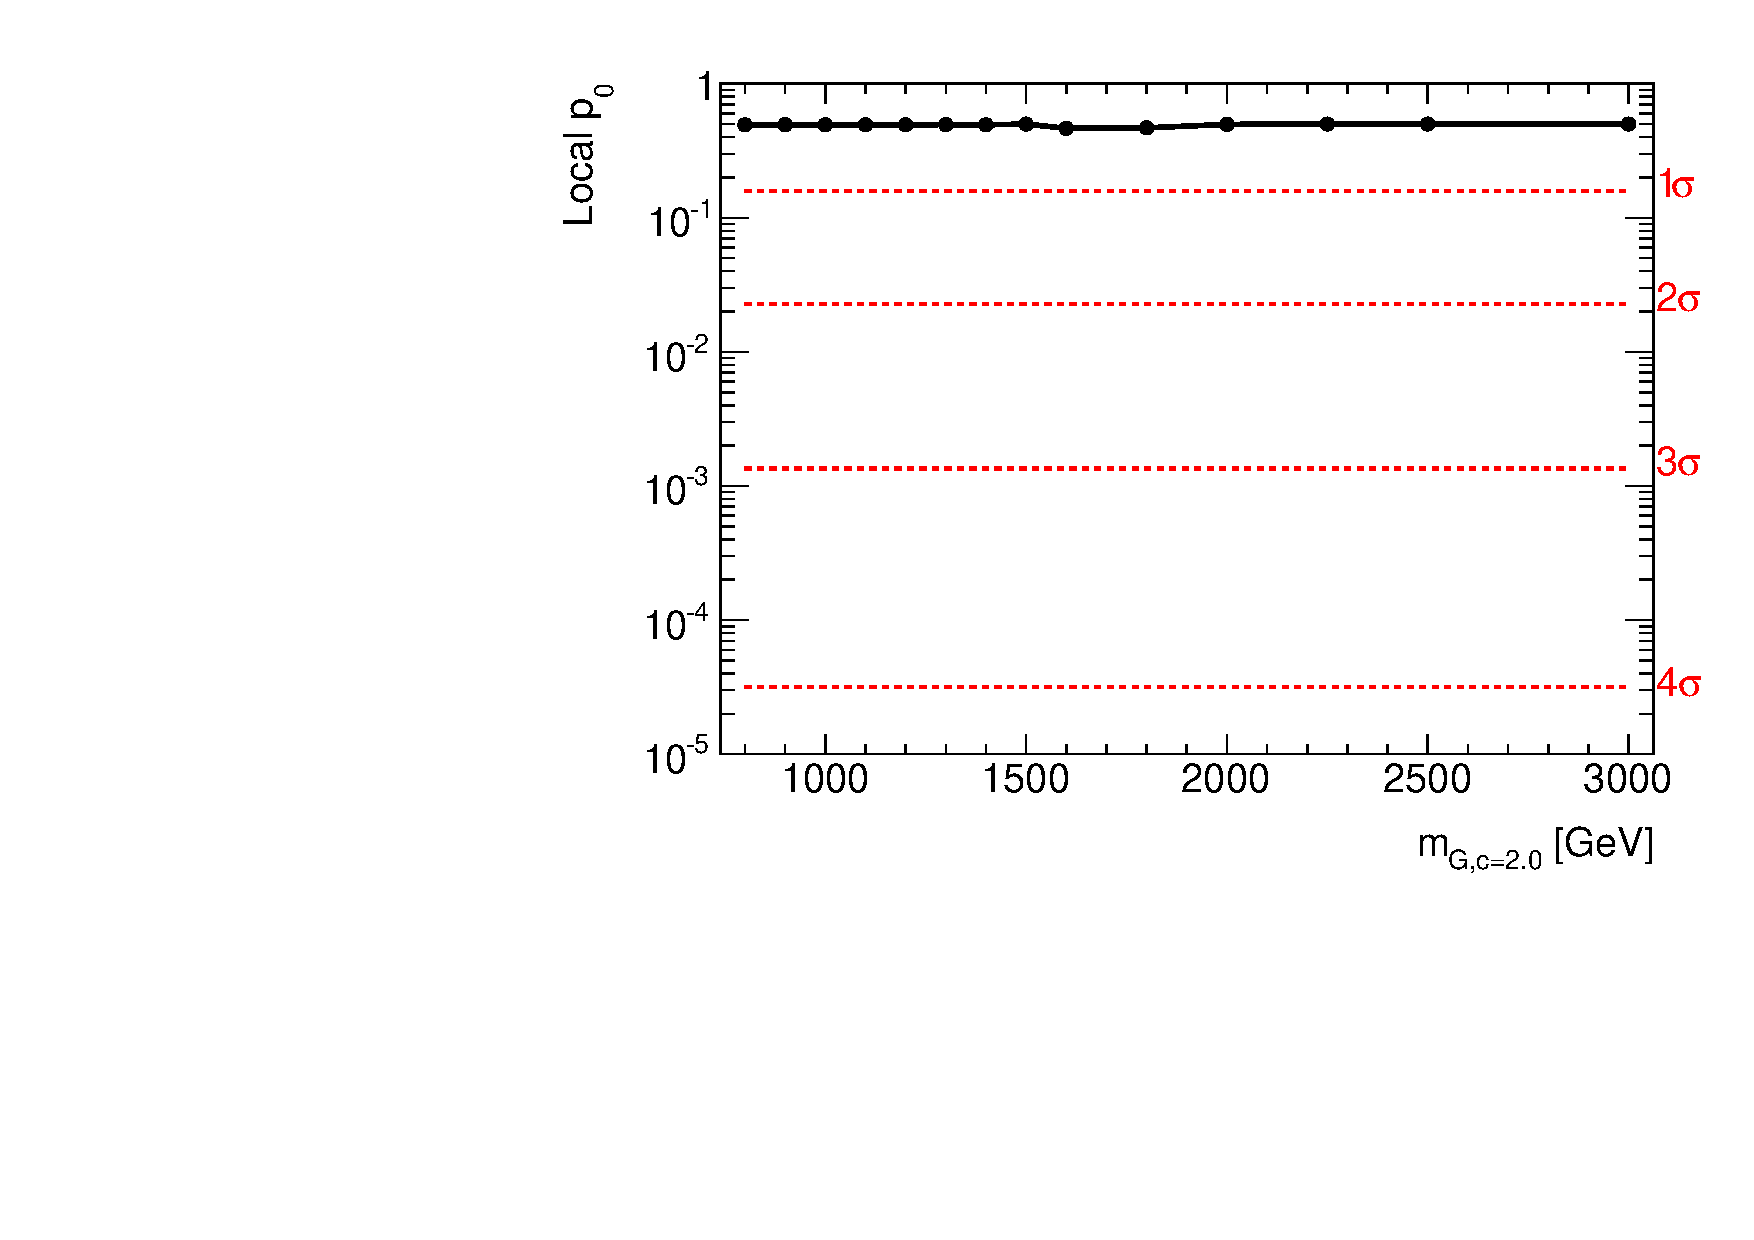
\includegraphics[width=0.21\textwidth,angle=-90]{figures/boosted/results/p0_g20_allmasses_boosted.pdf} 
\caption{Local $p_0$ of the (a) scalar, (b) c=1 Graviton and (c) c=2 Graviton.}
\label{fig:localp0}
\end{center}
\end{figure*}


\section{Resolved signal region}
\paragraph{}
The number of events observed in the data, the predicted number of background events in the signal region, and the predicted yield for three potential signals are presented in Table~\ref{tab:resolvedResults} for both the 2015 and 2016 datasets. The numbers of observed and predicted events in the control region are also given, and they are in agreement. A discrepancy between data and the total prediction is seen in the 2016 dataset; about half of this excess can be attributed to one bin at $\mfourj=280$~\GeV.

\begin{table}[!ht]
\begin{center}
\caption{The number of predicted background events in the signal region (SR) for the resolved analysis compared to the data, for the 2015 and 2016 datasets. The yields for three potential signals, an 800~\GeV\ \Grav resonance with \kMPl = 1, a scalar with a mass of 280~\GeV, and SM non-resonant Higgs boson pair production, are also shown. The scalar sample is normalized to a cross section times branching ratio of 2.7~pb. The quoted uncertainties include both the statistical and systematic uncertainties, and the total uncertainty considers correlations. The numbers of observed and predicted events are also given in the control region (CR).}

\begin{tabular}{c|c|c|c|c} 

Sample & 2015 SR & 2016 SR & 2015 CR & 2016 CR\\

Multijet                & 866     $\pm$  70      &  6750 $\pm$ 170  & 880 $\pm$ 71 & 7110 $\pm$ 180 \\
\ttbar, hadronic        &  52     $\pm$  35      & 259   $\pm$ 57   & 56  $\pm$ 37 & 276  $\pm$ 61 \\
\ttbar, semileptonic    &  13.9   $\pm$  6.5     &  123  $\pm$  30  & 20  $\pm$ 9  & 168 $\pm$ 40 \\
Total         & 930 $\pm$ 70      & 7130 $\pm$ 130  & 956 $\pm$ 50 &  7550 $\pm$ 130 \\
Data         & 928    & 7430 & 969 &7656  \\
\Grav$\left(800~\GeV\right)$ & 12.5   & 1.9     &  89  & 14 \\
Scalar (280~\GeV)            & 24     & 7.5     & 180  & 57 \\
SM di-Higgs                       & 0.607  & 0.091   & 4.43 & 0.66 \\

\end{tabular}
\label{tab:resolvedResults}
\end{center}
\end{table}

Figure~\ref{fig:resolvedHHUnblinded} shows comparisons of the predicted \mfourj~background distributions to those observed in the 2015 and 2016 datasets. A few signal models are also displayed. The scalar sample shown is normalized to a cross section times \hbb\ branching ratio of 2.7~pb, which is the best-fit value (the fit is described in Section~\ref{sec:statAna}). The predicted background and observed distributions are mostly in agreement, with an excess above the predicted background in one bin around 280~\GeV, which is discussed in Section~\ref{sec:statAna}.

\begin{figure}[!ht]
\begin{center}
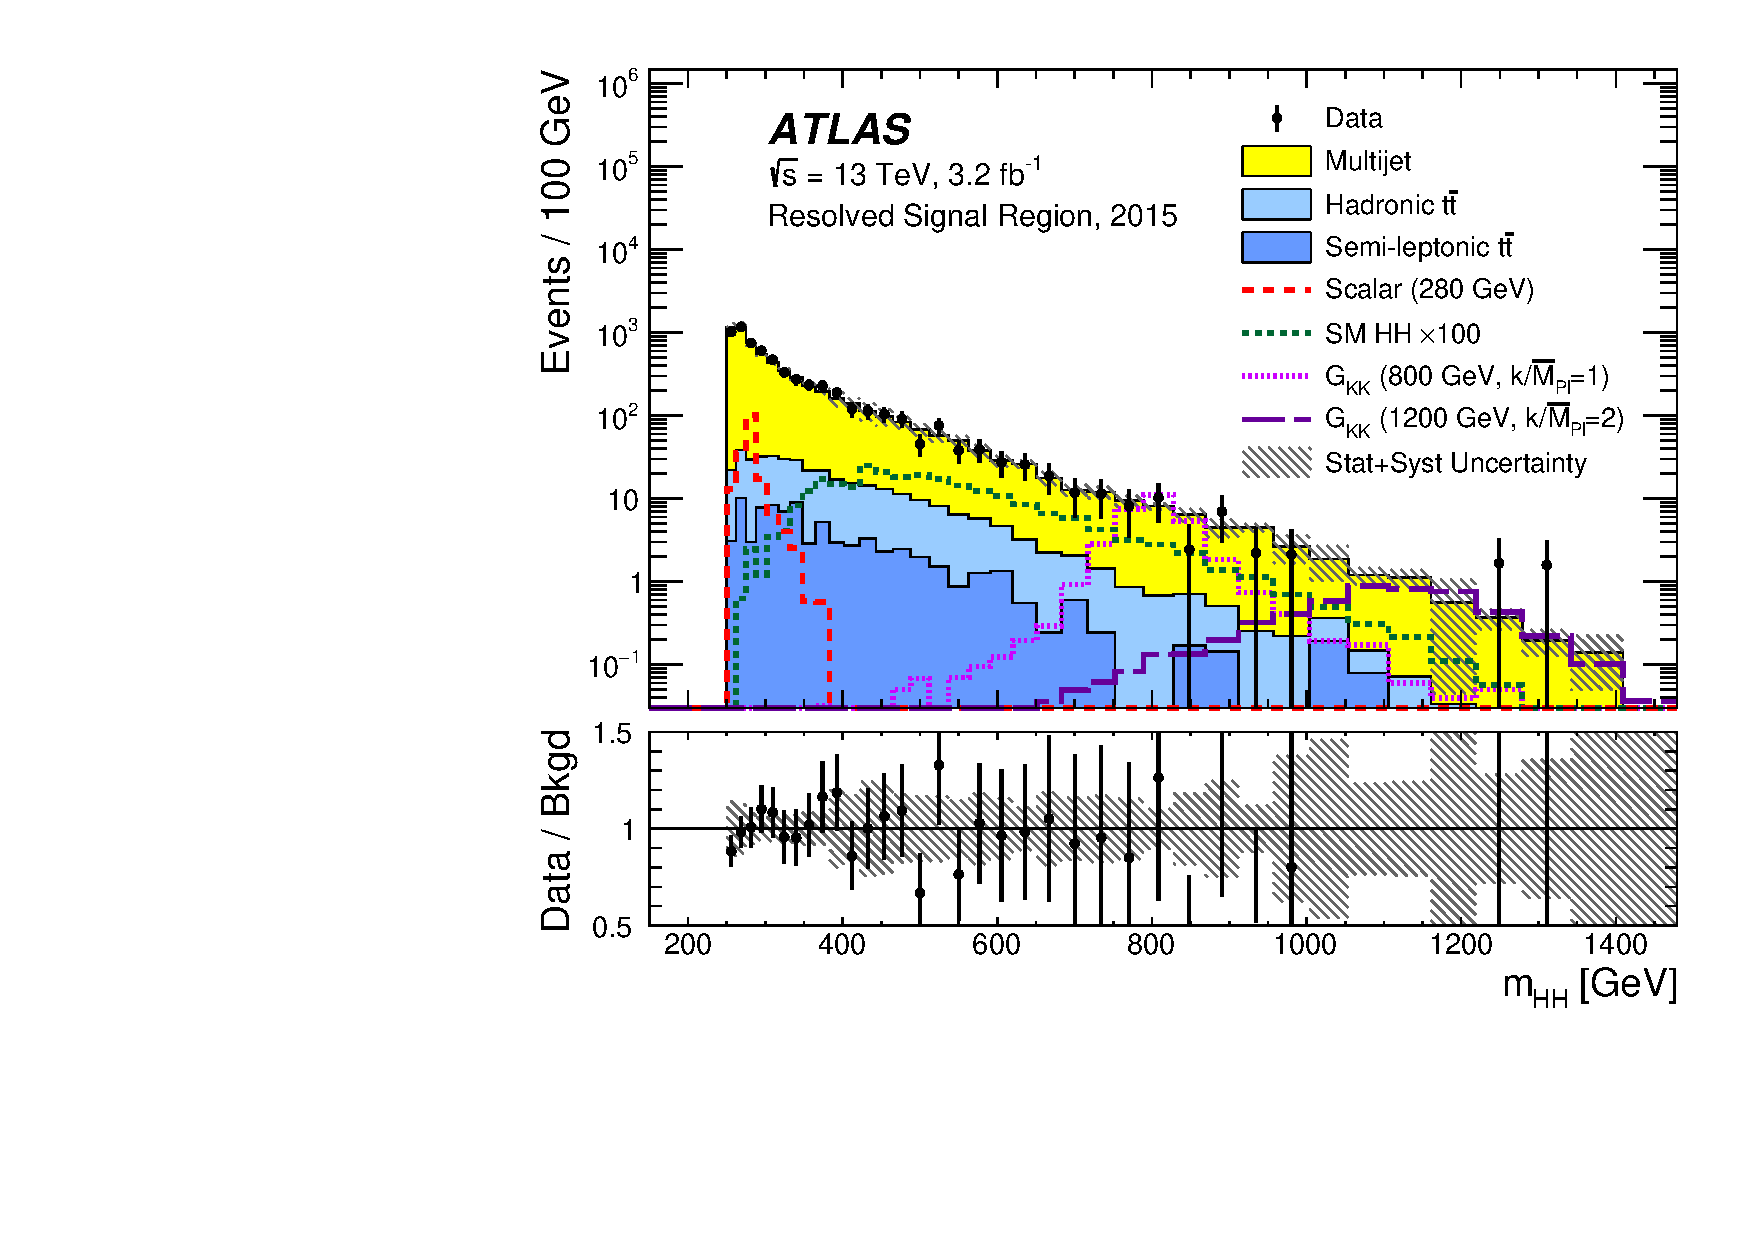
\includegraphics[width=0.3\textwidth,angle=-90]{figures/resolved/results/data_2015_hh_v_logy.pdf}
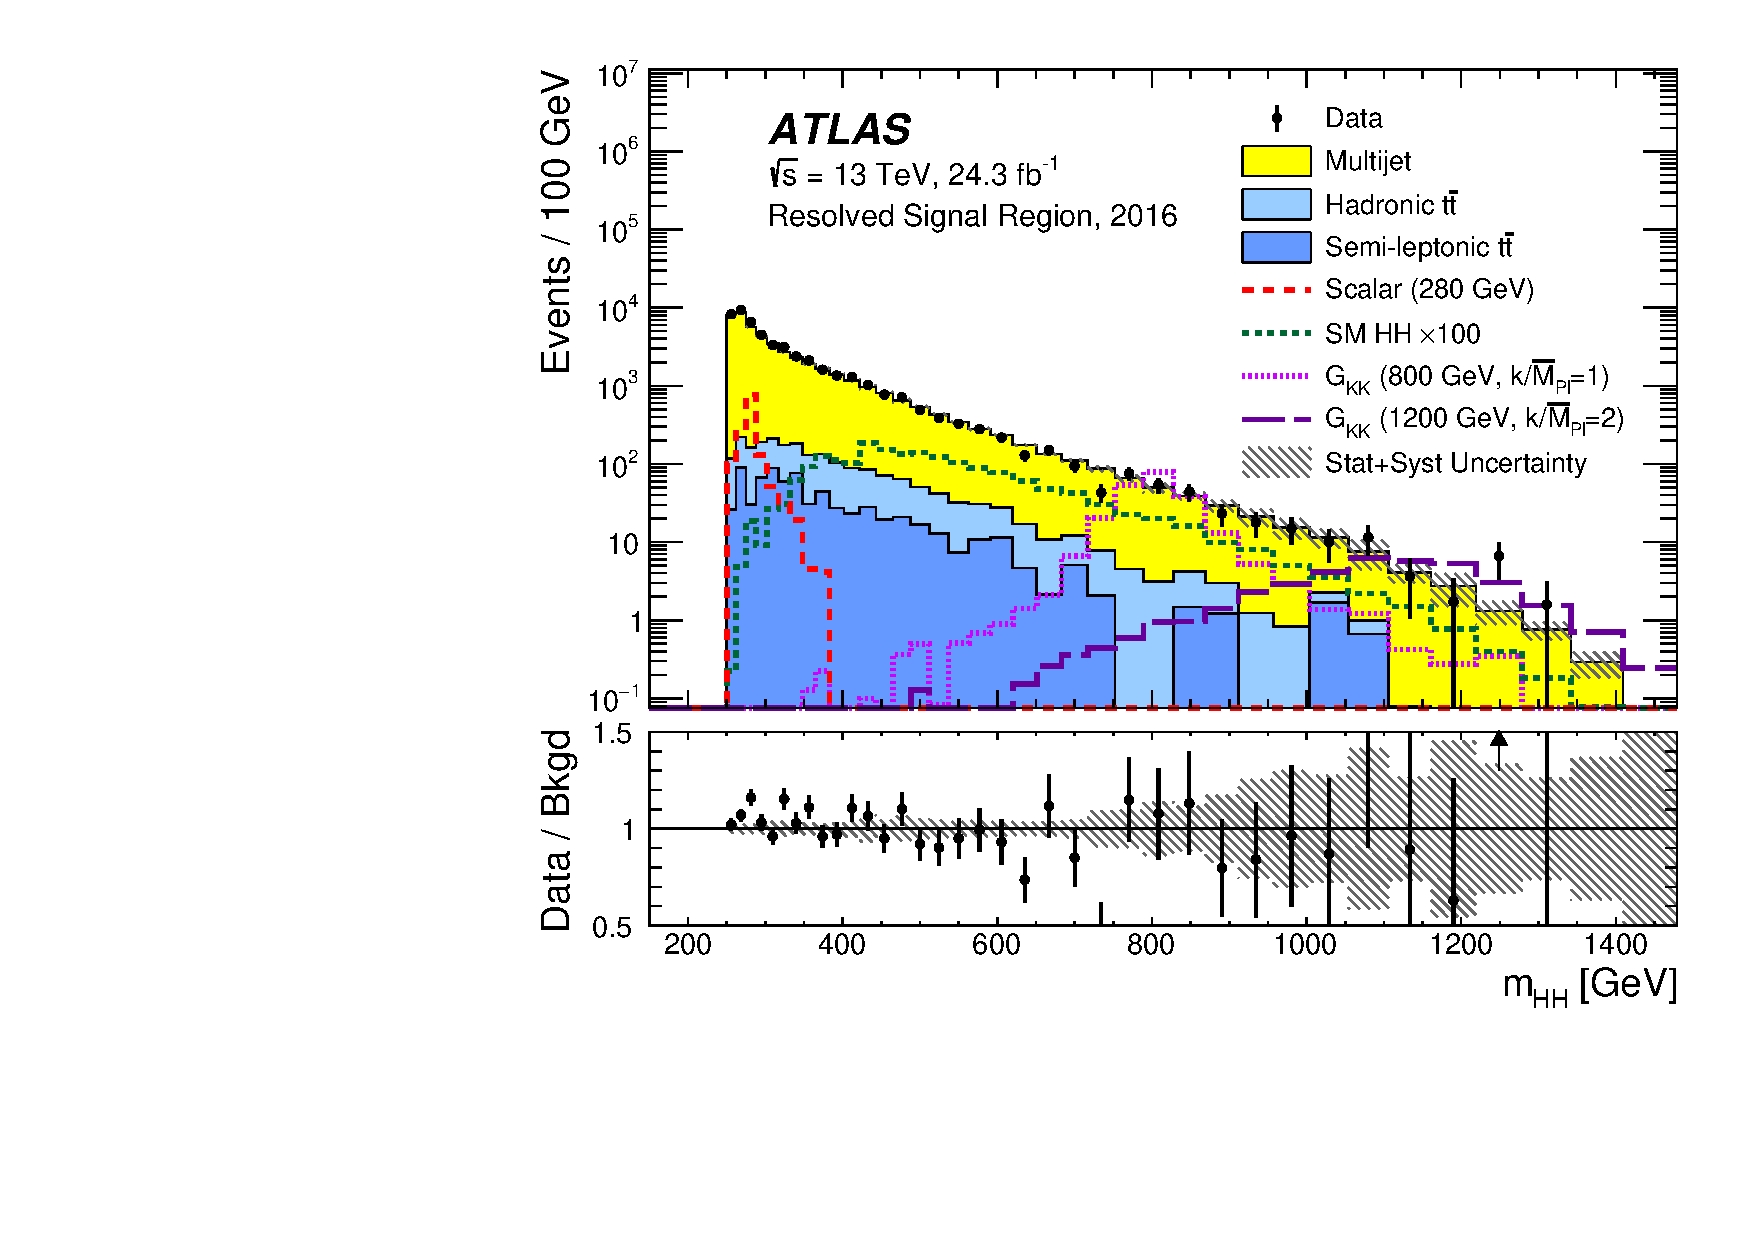
\includegraphics[width=0.3\textwidth,angle=-90]{figures/resolved/results/data_2016_hh_v_logy.pdf}
\caption{Distributions of \mfourj in the signal region of the resolved analysis for (a) 2015 data and (b) 2016 data, compared to the predicted backgrounds. The hatched bands shown in the bottom panels represent the combined statistical and systematic uncertainties in the total background estimates. The expected signal distributions of \Grav\ resonances with masses of 800 and 1200~\GeV, the 280~\GeV\ scalar sample and SM non-resonant di-Higgs production $(\times 100)$ are also shown. The scalar sample is normalized to a cross section times branching ratio of 2.7~pb.}
\label{fig:resolvedHHUnblinded}
\end{center}
\end{figure}


\section{Observed Limits}
\label{sec:observedlimits}

\paragraph{}
The observed limit for the narrow scalar is shown in Fig.~\ref{fig:limit_scalar}. The stat-only limit is also shown. The impact of systematic uncertainties is small. The observed limits for the Graviton models is shown in Fig.~\ref{fig:limit_g10} for c=1 and in Fig.~\ref{fig:limit_g20} for c=2. These limits do not contain any of the resolved categories.

\begin{figure*}
\begin{center}
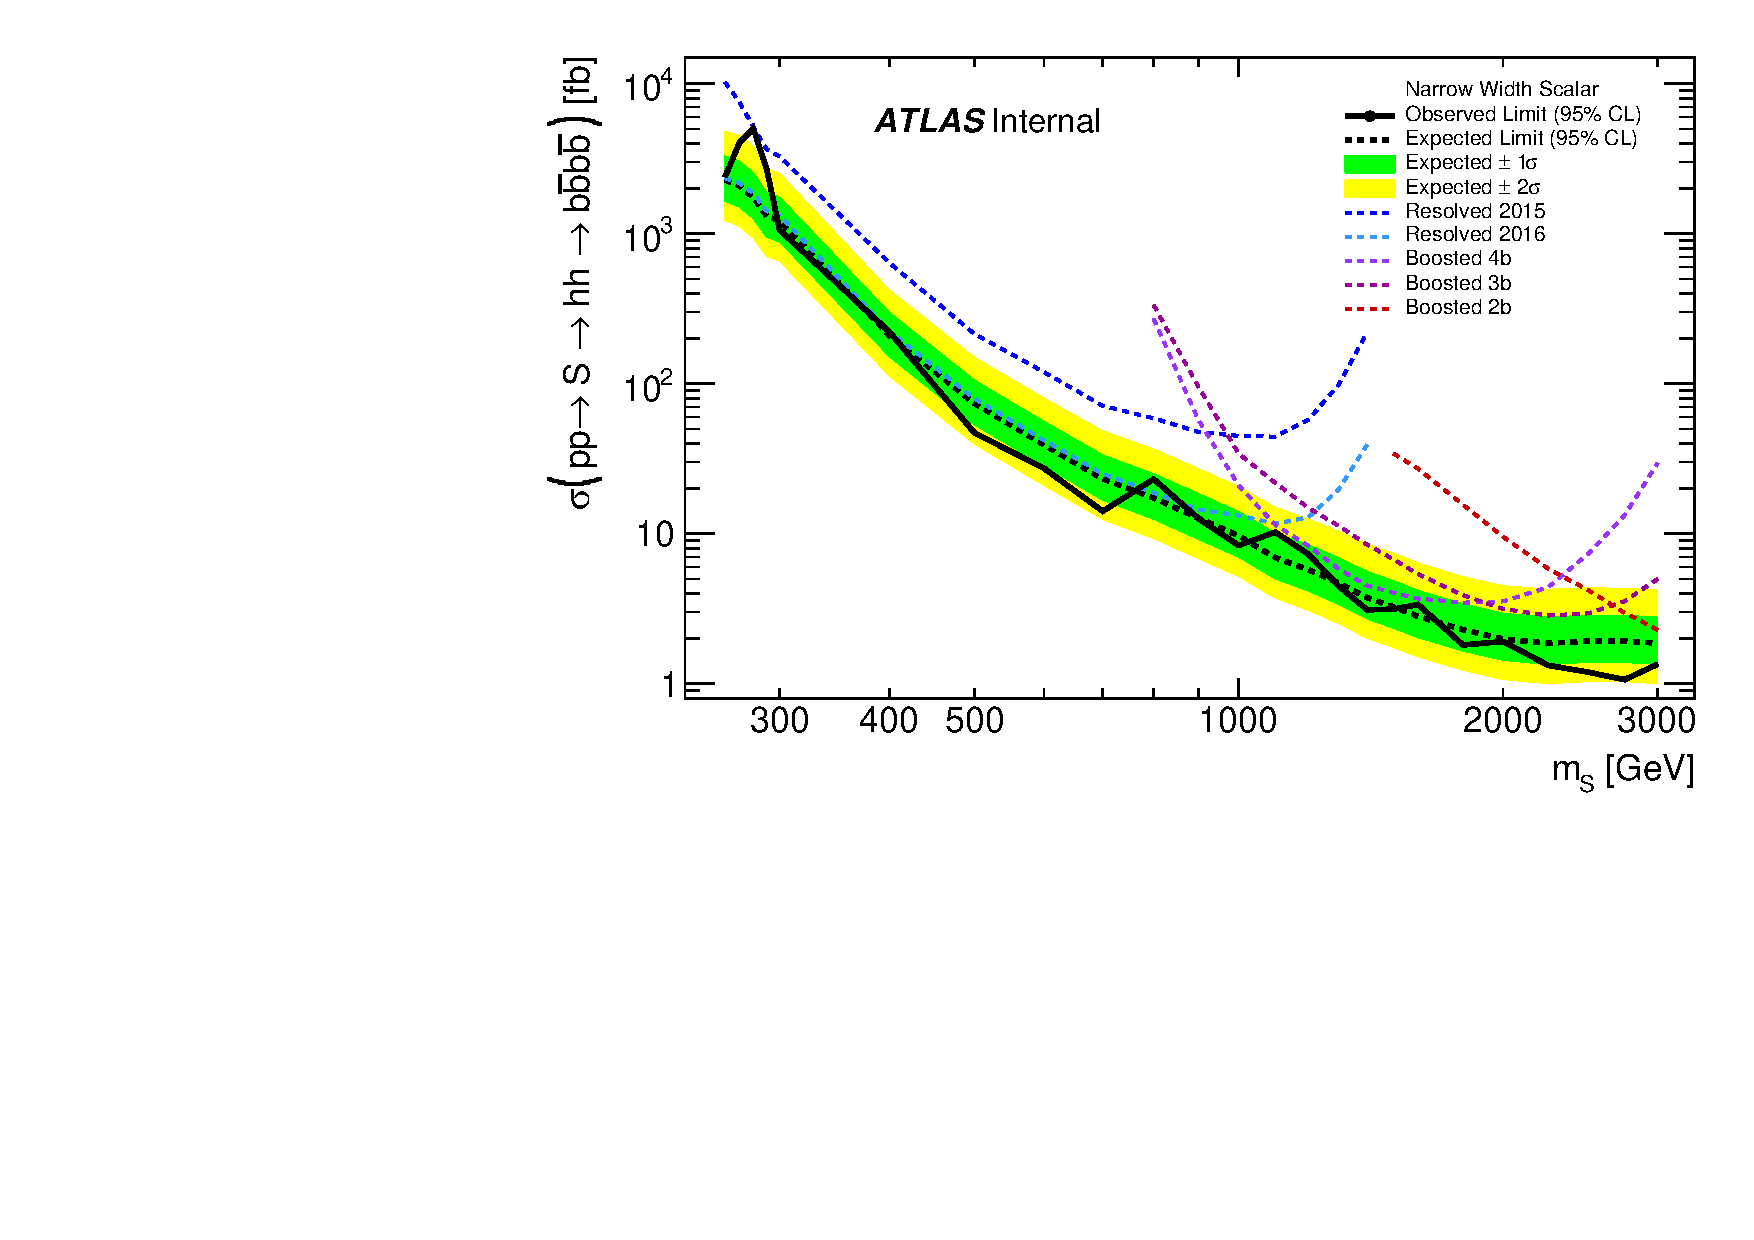
\includegraphics[width=0.4\textwidth,angle=-90]{figures/boosted/results/BrazilPlot_Asymptotic_s_hh_combined_AllSyst_unblinded_2017-10-04.pdf}
\caption{The expected and observed 95\% C.L. upper exclusion limits for the boosted $4b$ analysis calculated including all systematic uncertainties for the narrow scalar model. The dot-dashed line shows the expected limit when only statistical uncertainties are included. The limits are derived within the asymptotic approximation.}
\label{fig:limit_scalar}
\end{center}
\end{figure*}

\begin{figure*}
\begin{center}
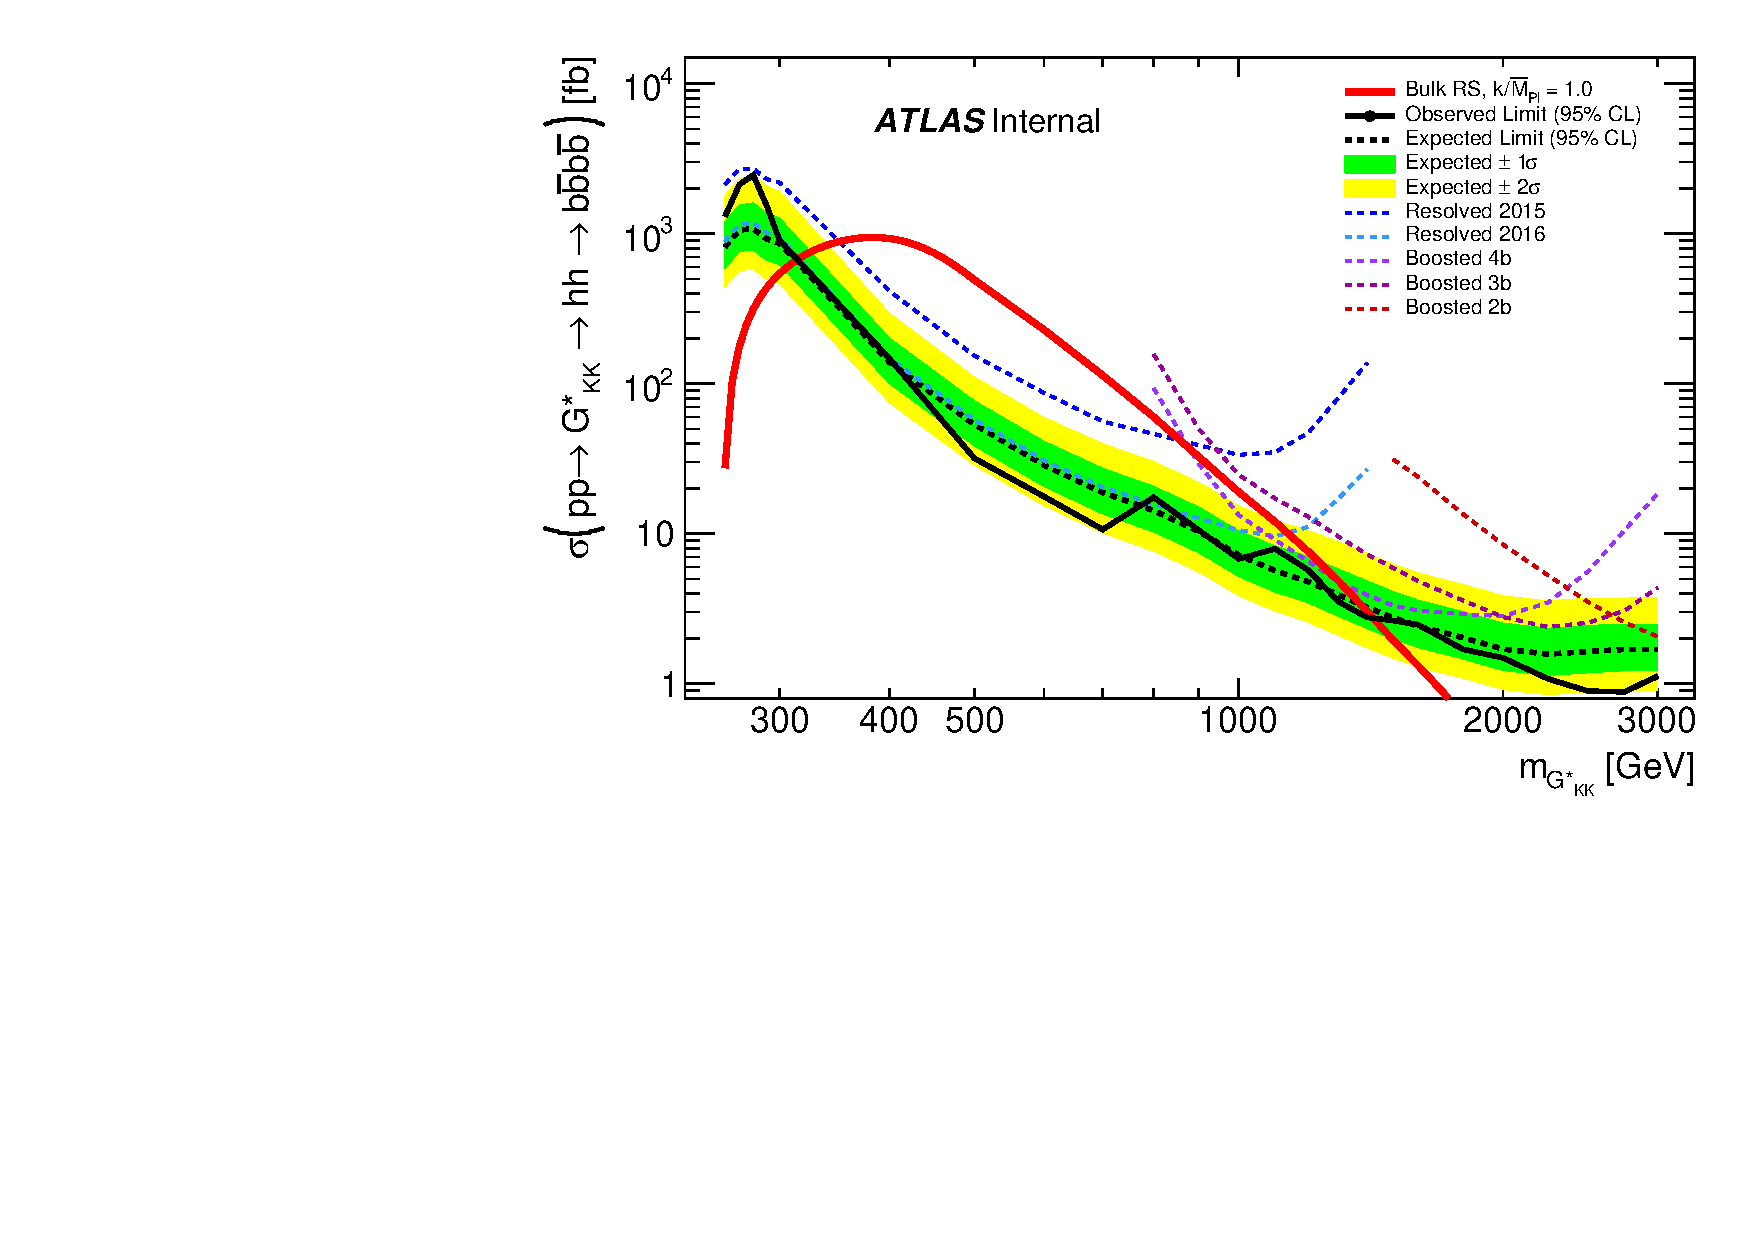
\includegraphics[width=0.4\textwidth,angle=-90]{figures/boosted/results/BrazilPlot_Asymptotic_g_hh_c10_combined_AllSyst_unblinded_2017-10-04.pdf}
\caption{The expected and observed 95\% C.L. upper exclusion limits for the boosted $4b$ analysis calculated including all systematic uncertainties for the c=1.0 Graviton. The dot-dashed line shows the expected limit when only statistical uncertainties are included. The limits are derived within the asymptotic approximation.}
\label{fig:limit_scalar}
\end{center}
\end{figure*}
\begin{figure*}

\begin{center}
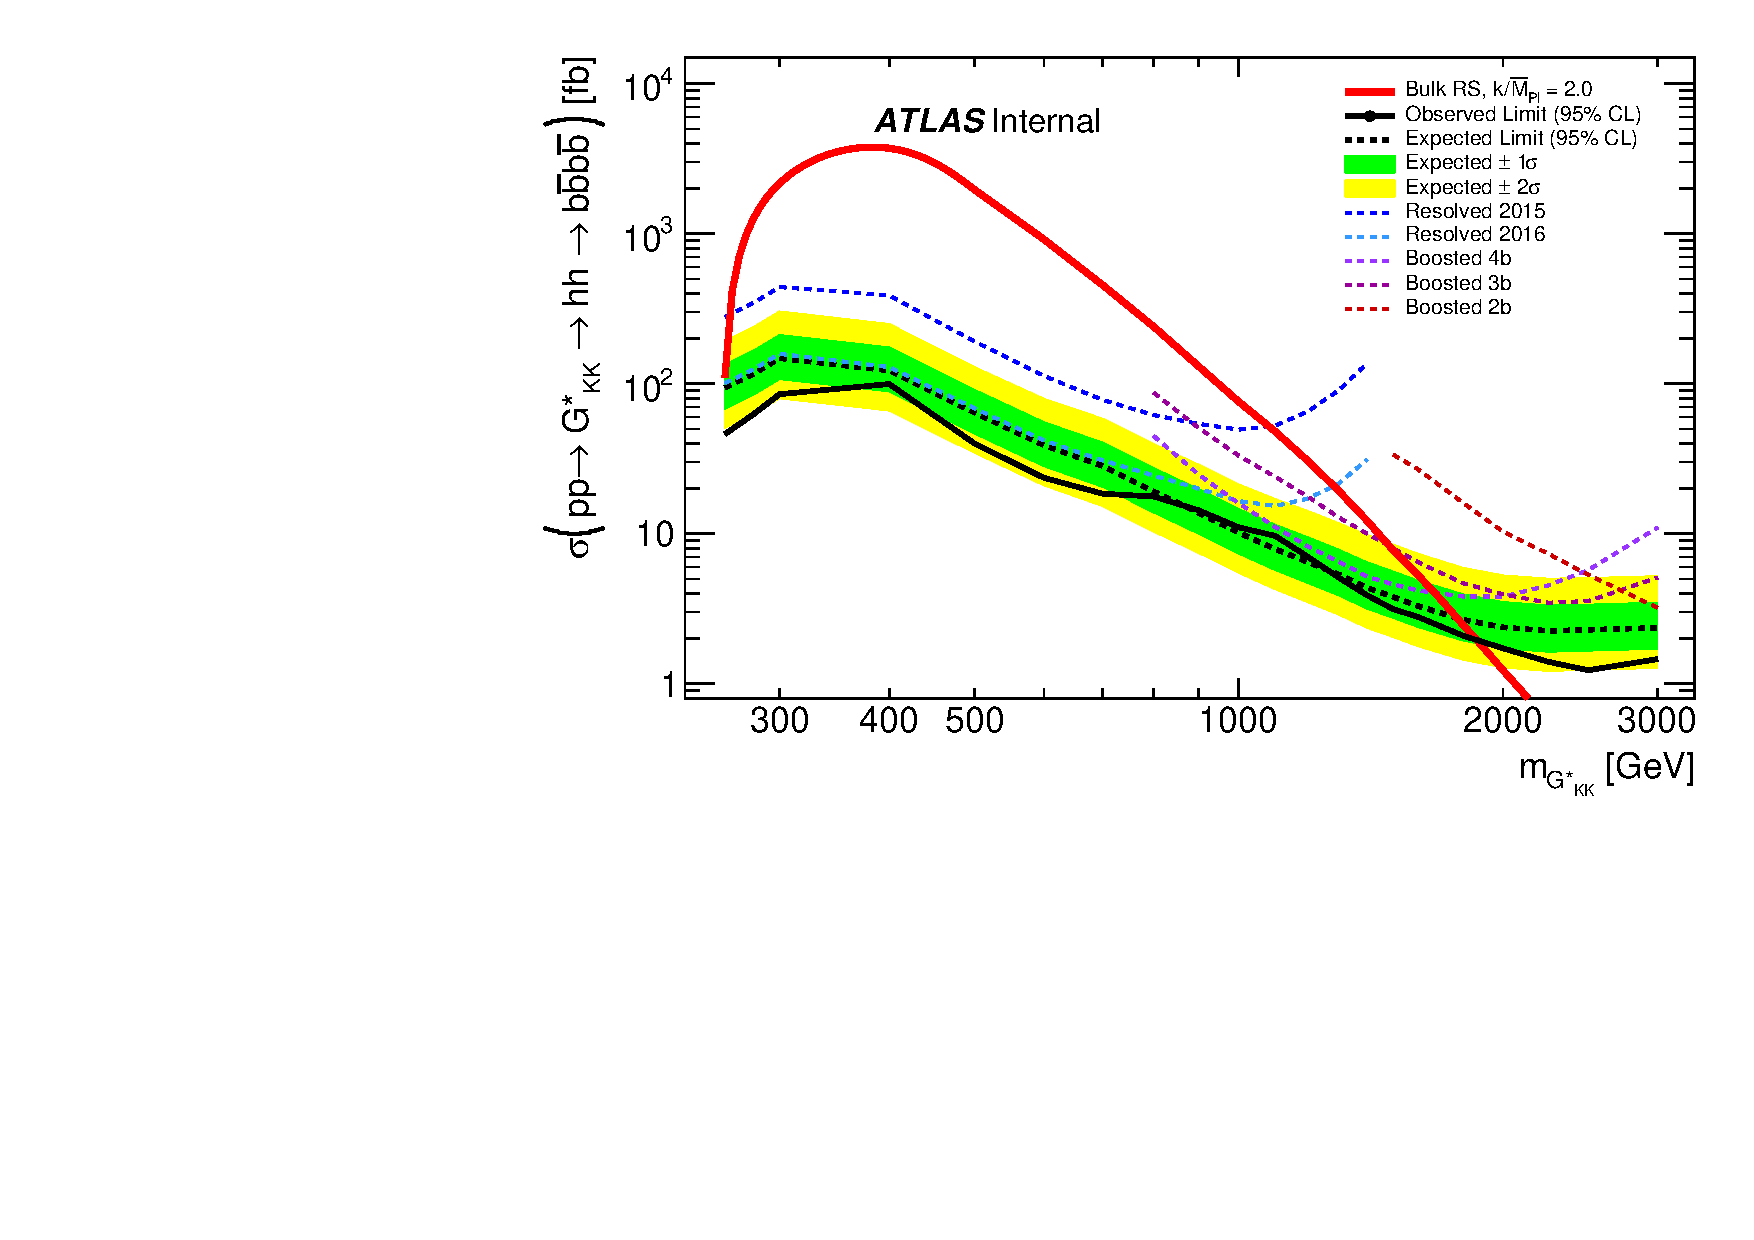
\includegraphics[width=0.4\textwidth,angle=-90]{figures/boosted/results/BrazilPlot_Asymptotic_g_hh_c20_combined_AllSyst_unblinded_2017-10-09.pdf}
\caption{The expected and observed 95\% C.L. upper exclusion limits for the boosted $4b$ analysis calculated including all systematic uncertainties for the c=2.0 Graviton. The dot-dashed line shows the expected limit when only statistical uncertainties are included. The limits are derived within the asymptotic approximation.}
\label{fig:limit_scalar}
\end{center}
\end{figure*}

Figure~\ref{fig:nuisanceParams} shows the pulls of the systematic uncertainty nuisance parameters and their correlations for the 2000 GeV mass point. One nuisance parameter (QCD\_ShapeCRHigh) in both the $2b$ and $3b$ samples shows a significant constraint coming from the signal region data. This nuisance parameter corresponds to the shape uncertainty on the QCD background derived from the $2b$ and $3b$ control regions, as explained in Section \ref{unc-shape-qcd-in-sr}. The prior probability distributions for this nuisance parameter is very broad, with the relative uncertainty on the background prediction reaching 15000\% at high $m_{hh}$. This is because there is very little data in the control region at high mass to constrain the uncertainty. In the signal region however, the two events found suffice to constrain it: very tightly in comparison to the extremely loose prior constraint.

\begin{figure*}[htbp!]
\begin{center}
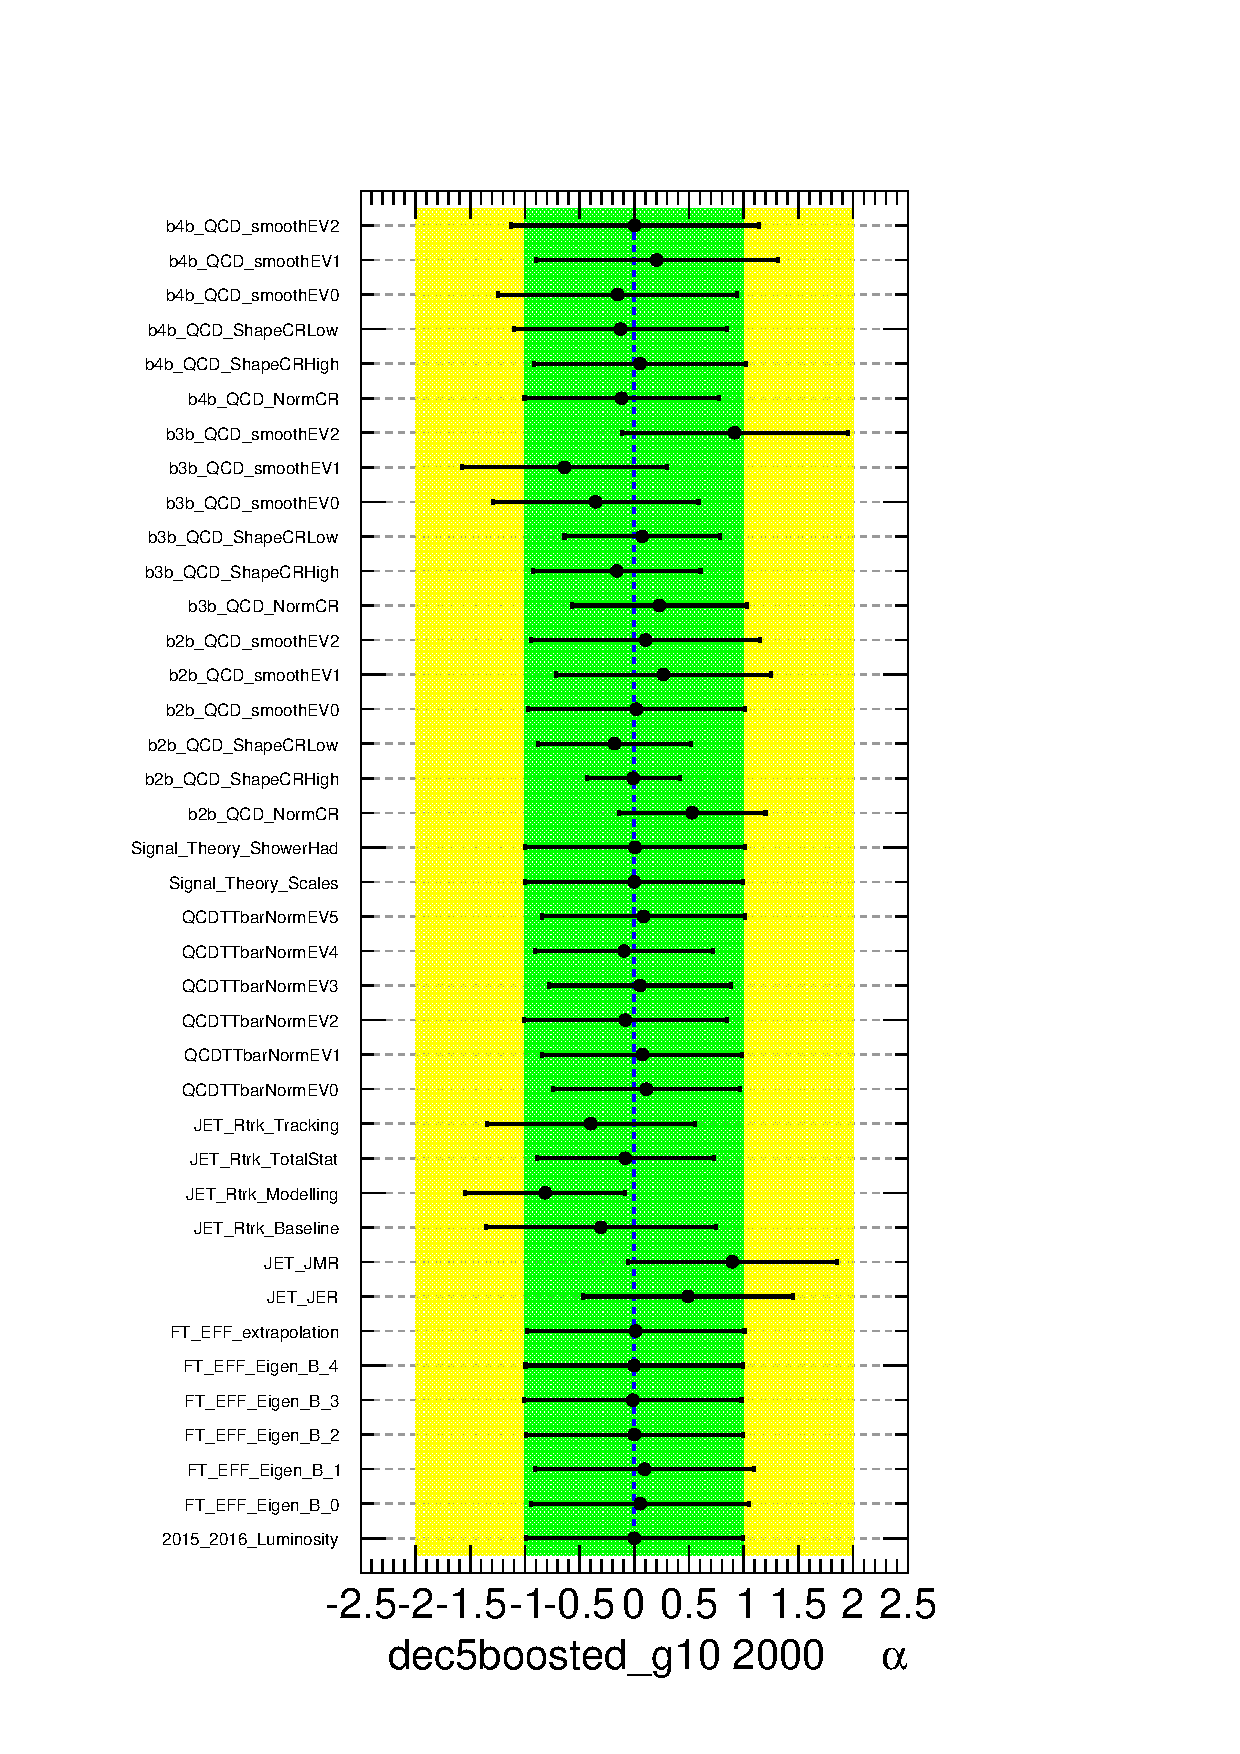
\includegraphics[width=0.39\textwidth,angle=-90]{figures/boosted/results/pulls_2000_data.pdf}
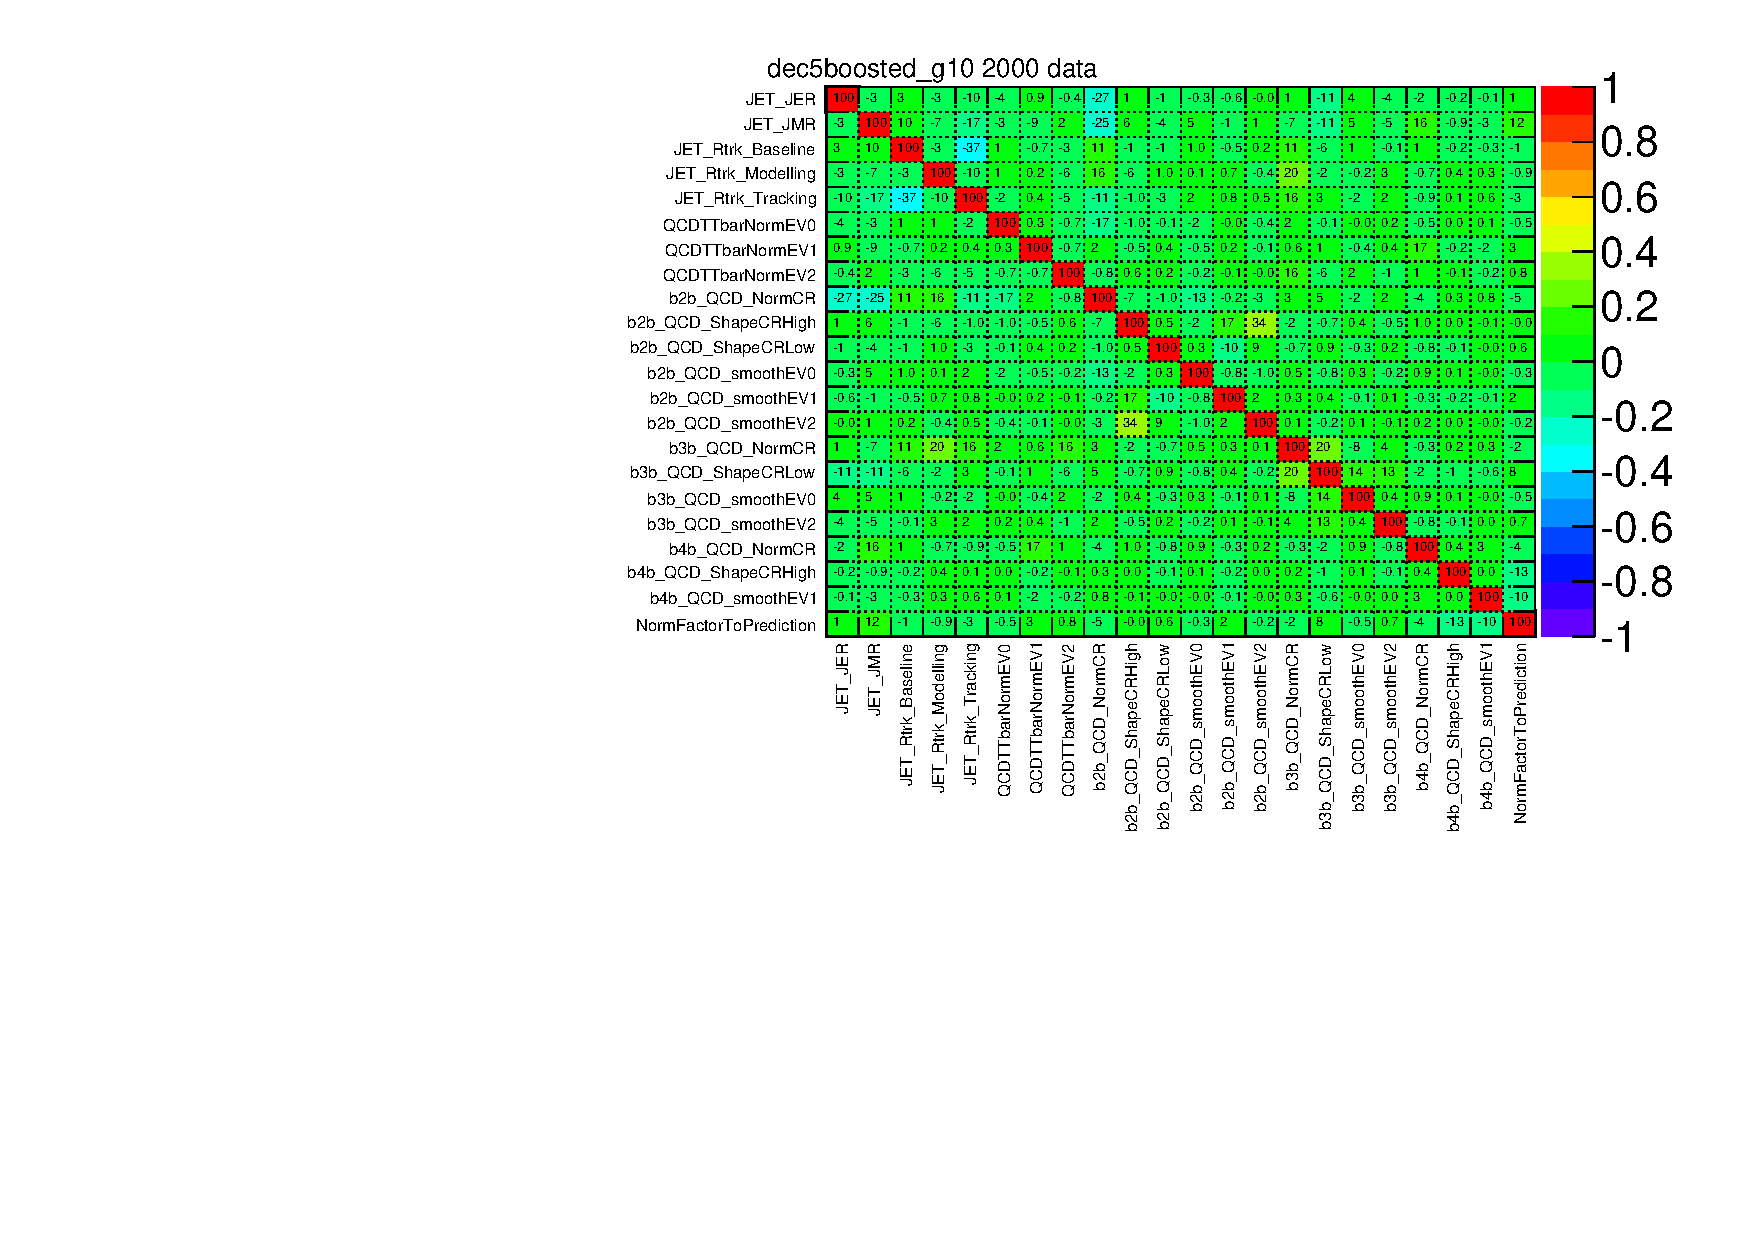
\includegraphics[width=0.59\textwidth,angle=-90]{figures/boosted/results/corr_2000_data.pdf}
\caption{Nuisance parameters associated with the background modelling, after the conditional likelihood fit for a bulk RS graviton signal with $\mGrav=2\,\TeV$ and $\kMPl=1.0$. The tight constraints of 2b\_QCD\_CRShape and 3b\_QCD\_CRShape are a result of the nuisance parameter prior being unconstrained due to a lack of control region data at high mass.}
\label{fig:nuisanceParams}
\end{center}
\end{figure*}

Examples of the fit used to set these limits are shown in Figures~\ref{fig:postfit2000} and~\ref{fig:postfit2500}, where a narrow scalar is used for the signal model. In the case the best-fit is negative, the fit is repeated with mu bounded to zero. This happens at several mass points, for example at 1.5, 2.5 and 3 TeV. At 2~TeV, the fitted signal is positive ($\mu=0.1\pm0.25$) though well consistent with the background-only hypothesis. In all fits, good agreement is seen between data and the background model.

\begin{figure*}[htbp!]
\begin{center}
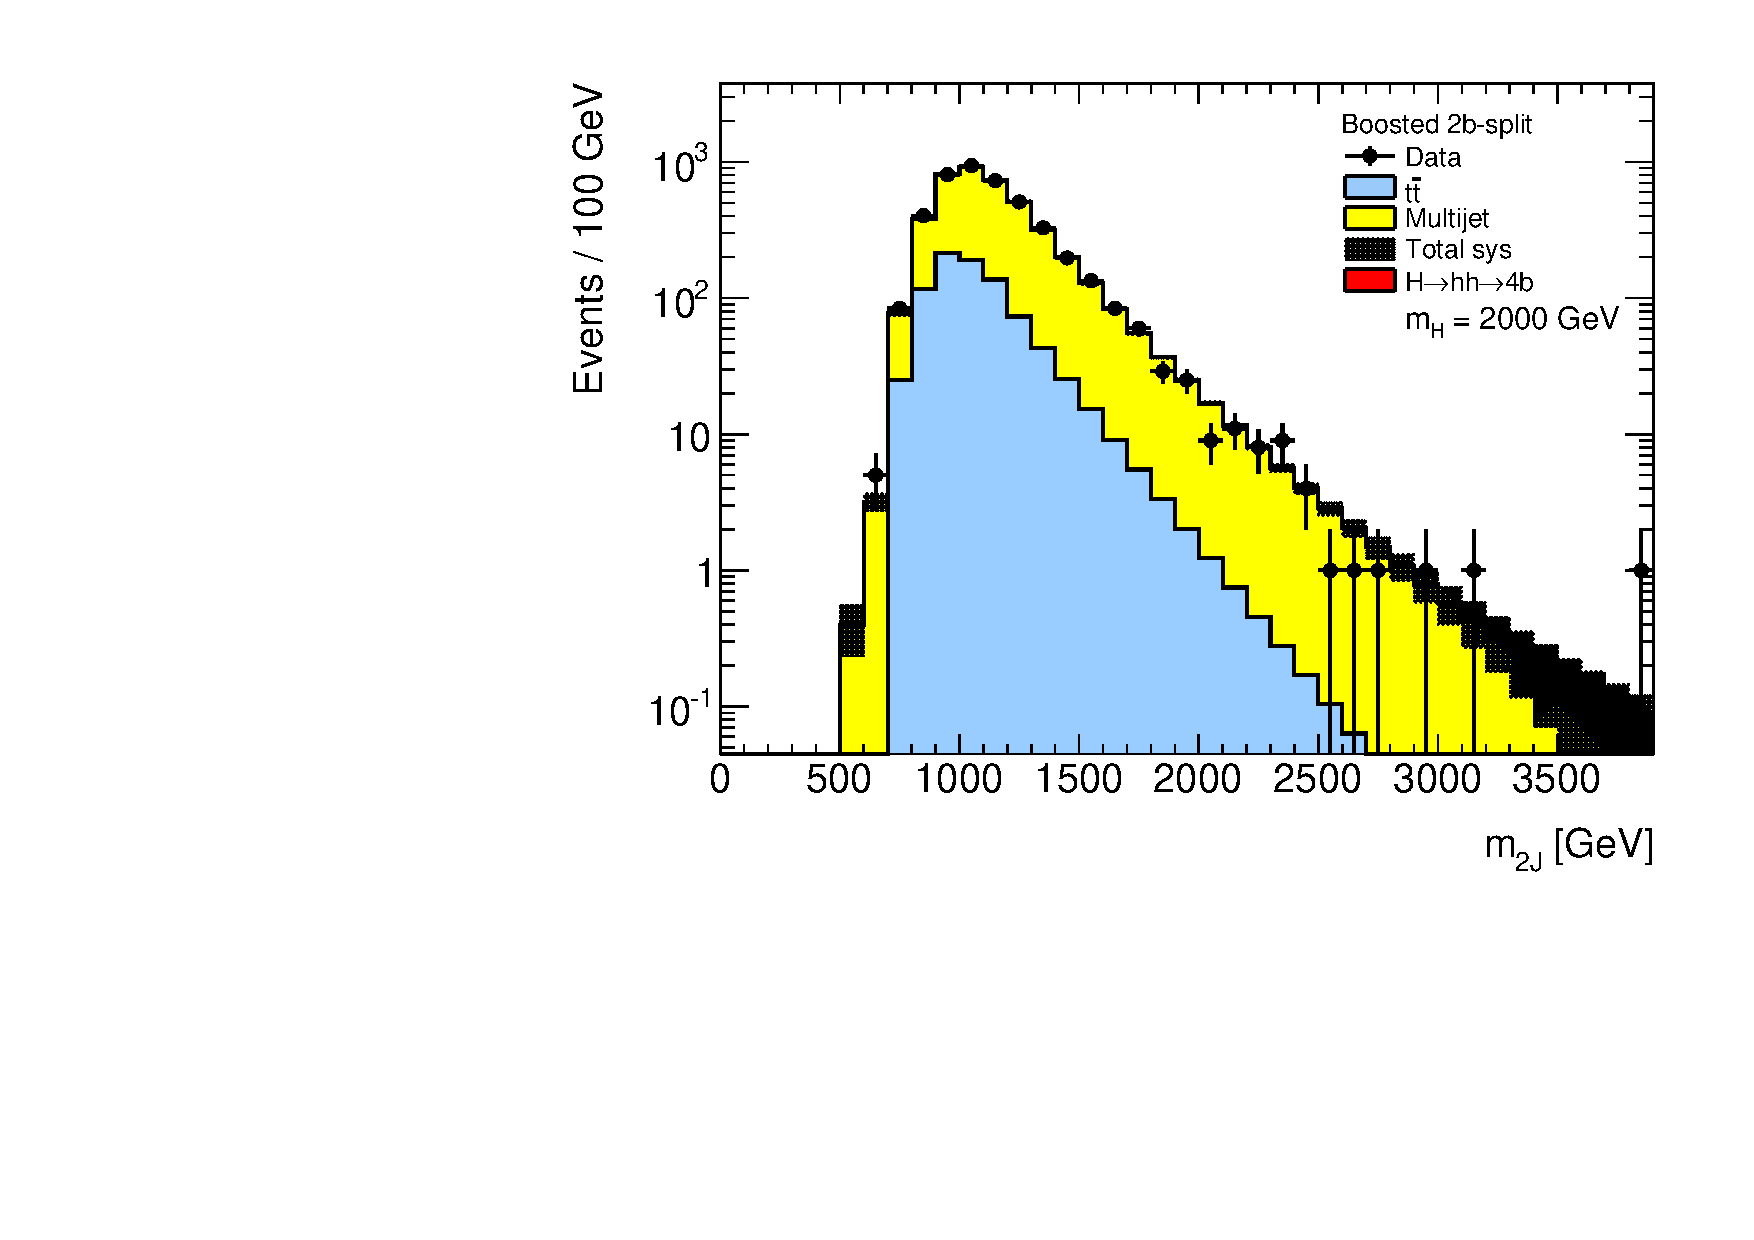
\includegraphics[width=0.21\textwidth,angle=-90]{figures/boosted/results/postfitplot_s_2000_b2b.pdf} 
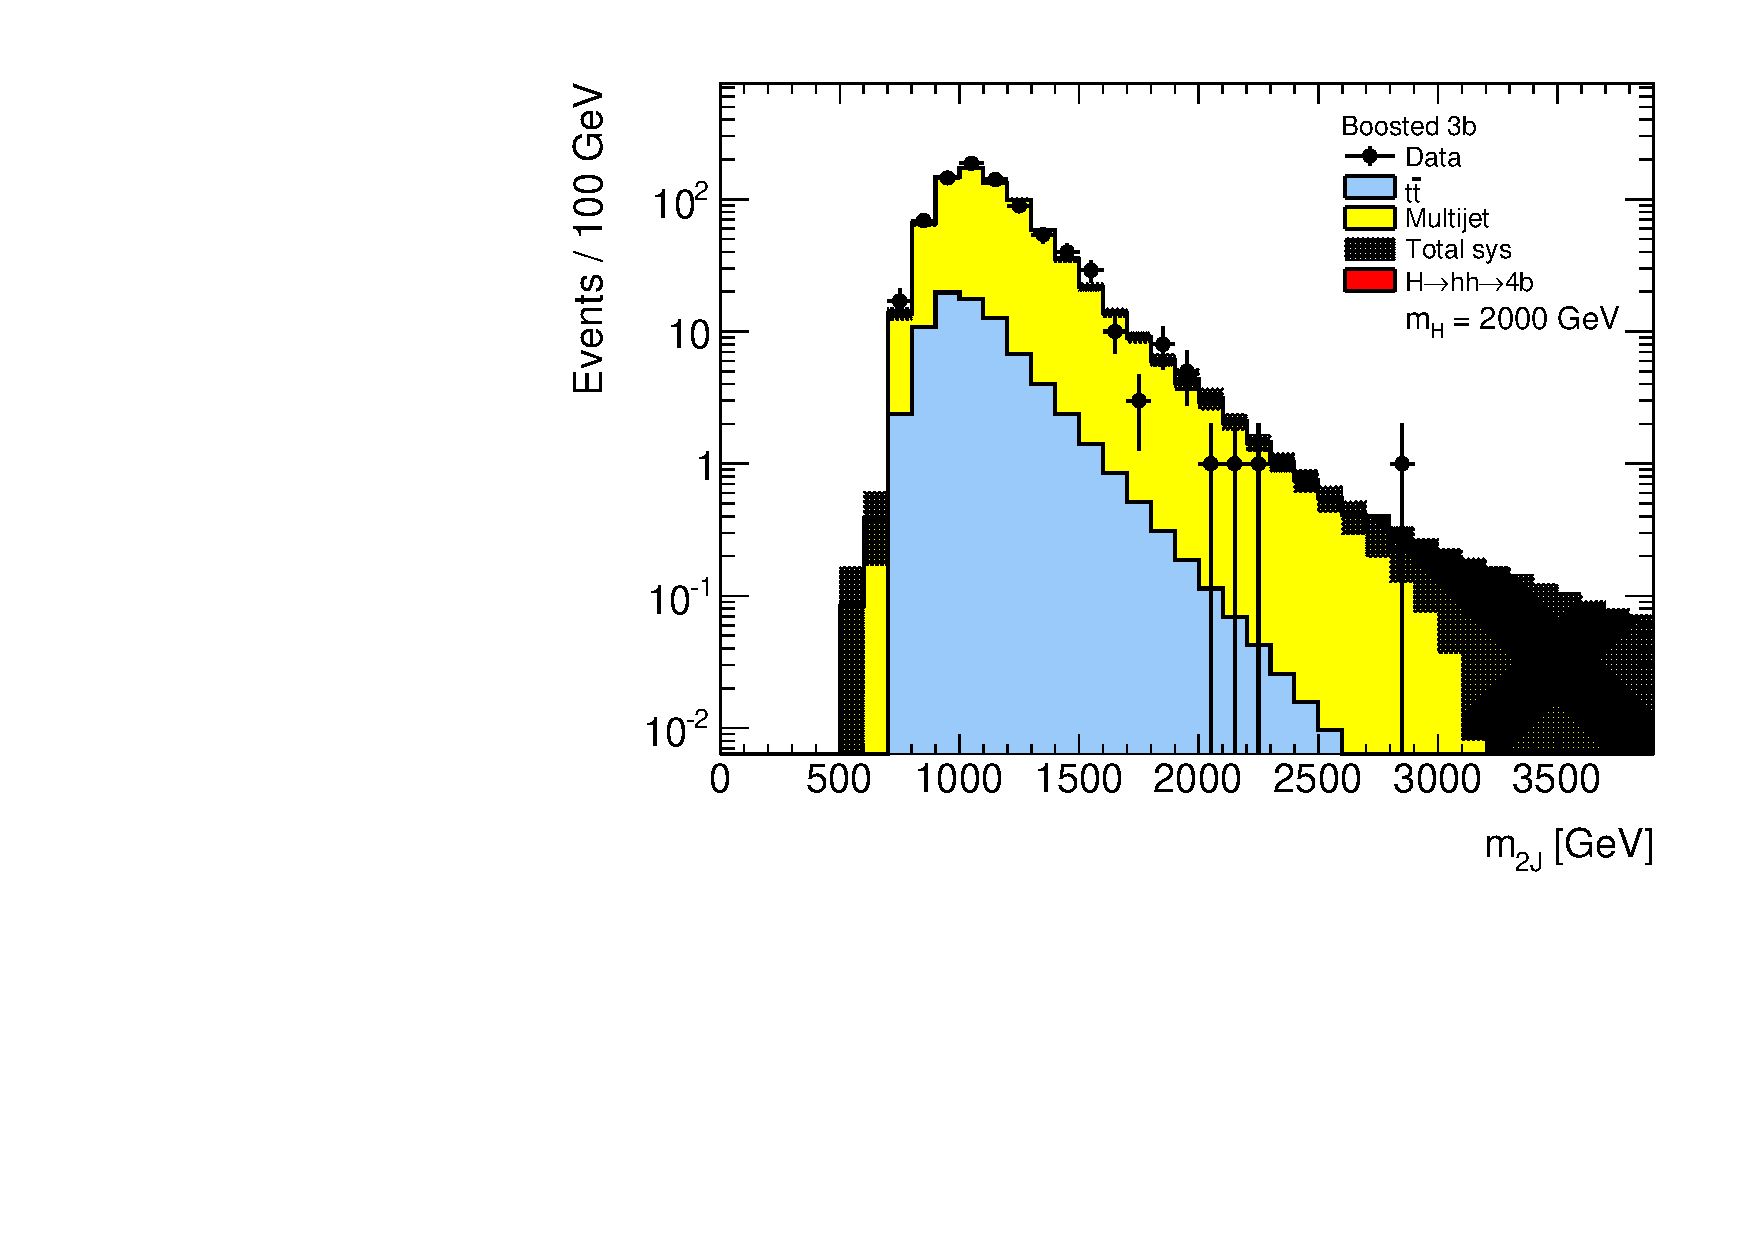
\includegraphics[width=0.21\textwidth,angle=-90]{figures/boosted/results/postfitplot_s_2000_b3b.pdf} 
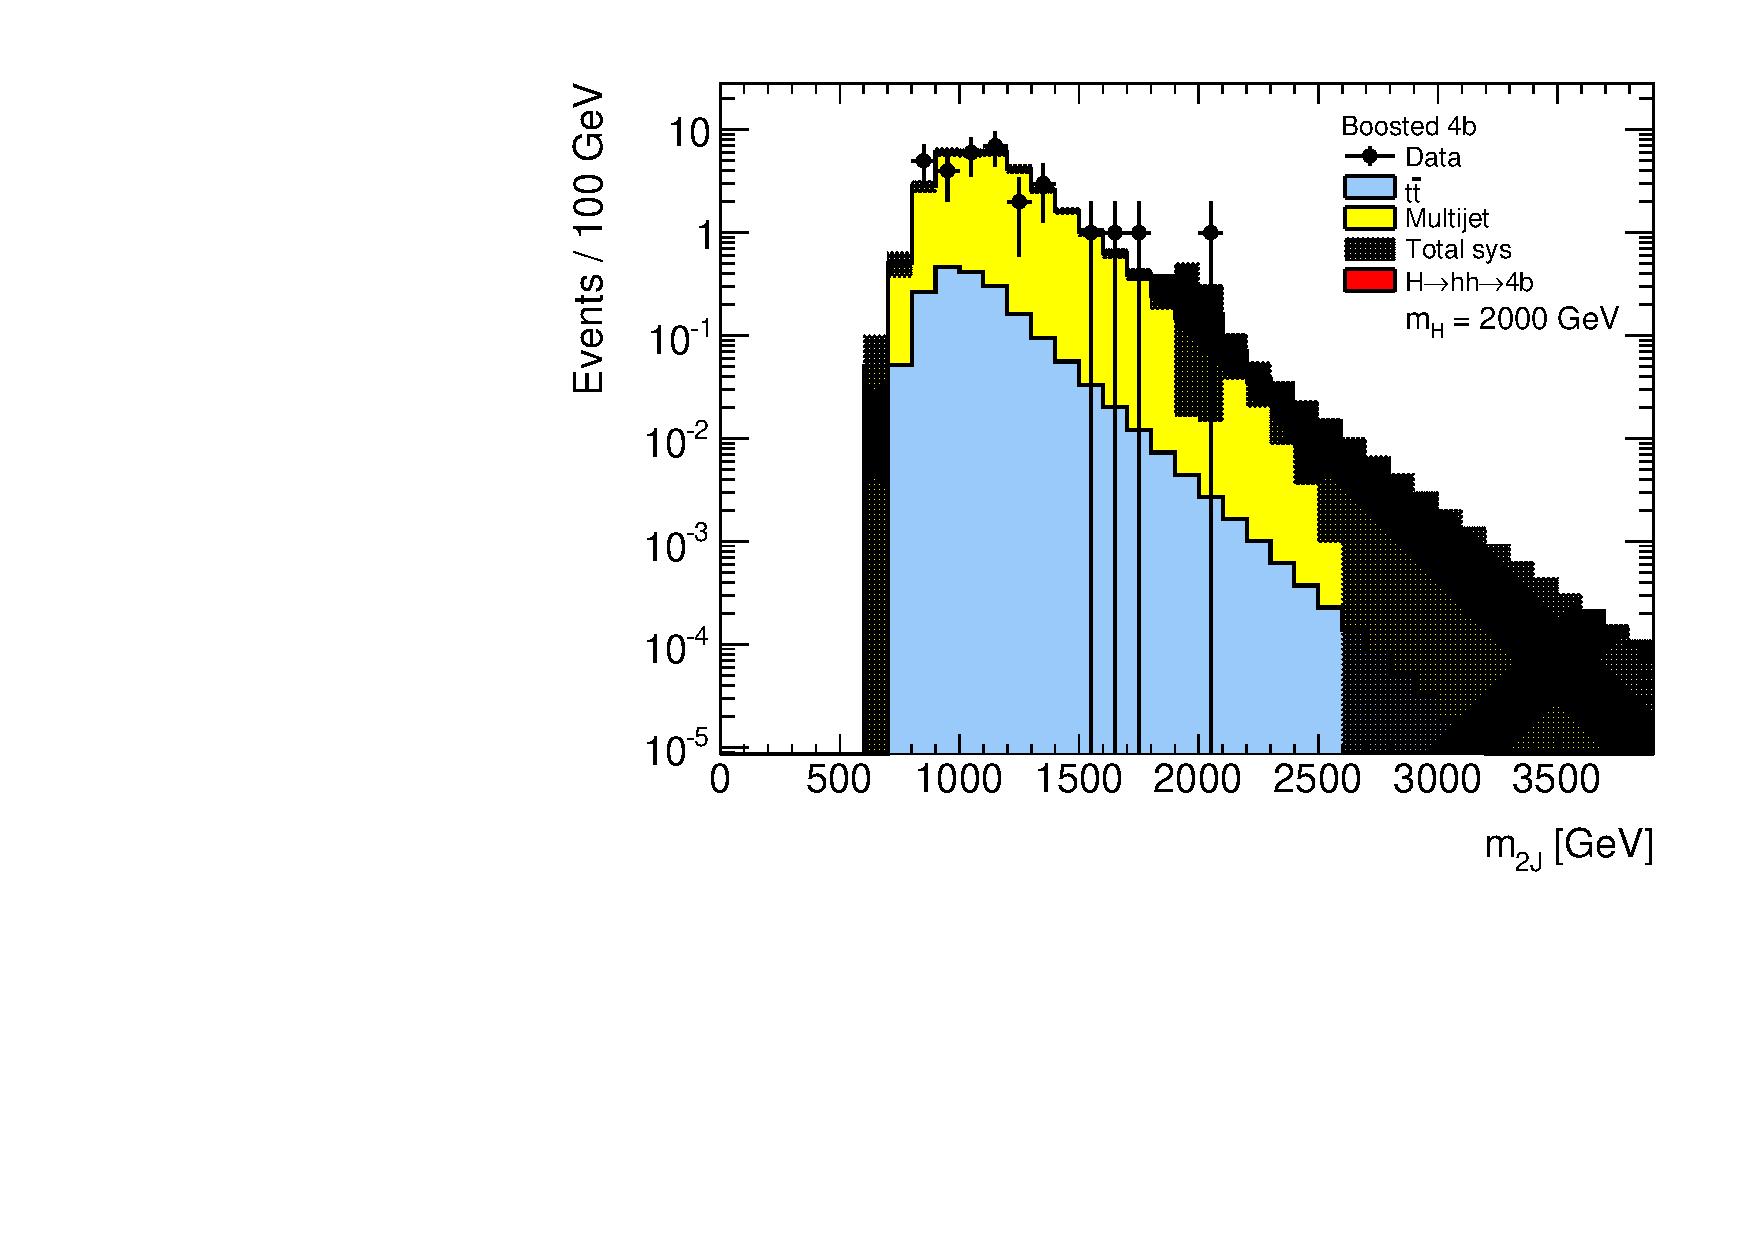
\includegraphics[width=0.21\textwidth,angle=-90]{figures/boosted/results/postfitplot_s_2000_b4b.pdf} 
\caption{Postfit distributions after fitting the data with the 2000 GeV signal hypothesis. The signal strenght is slightly positive.}
\label{fig:postfit2000}
\end{center}
\end{figure*}

\begin{figure*}[htbp!]
\begin{center}
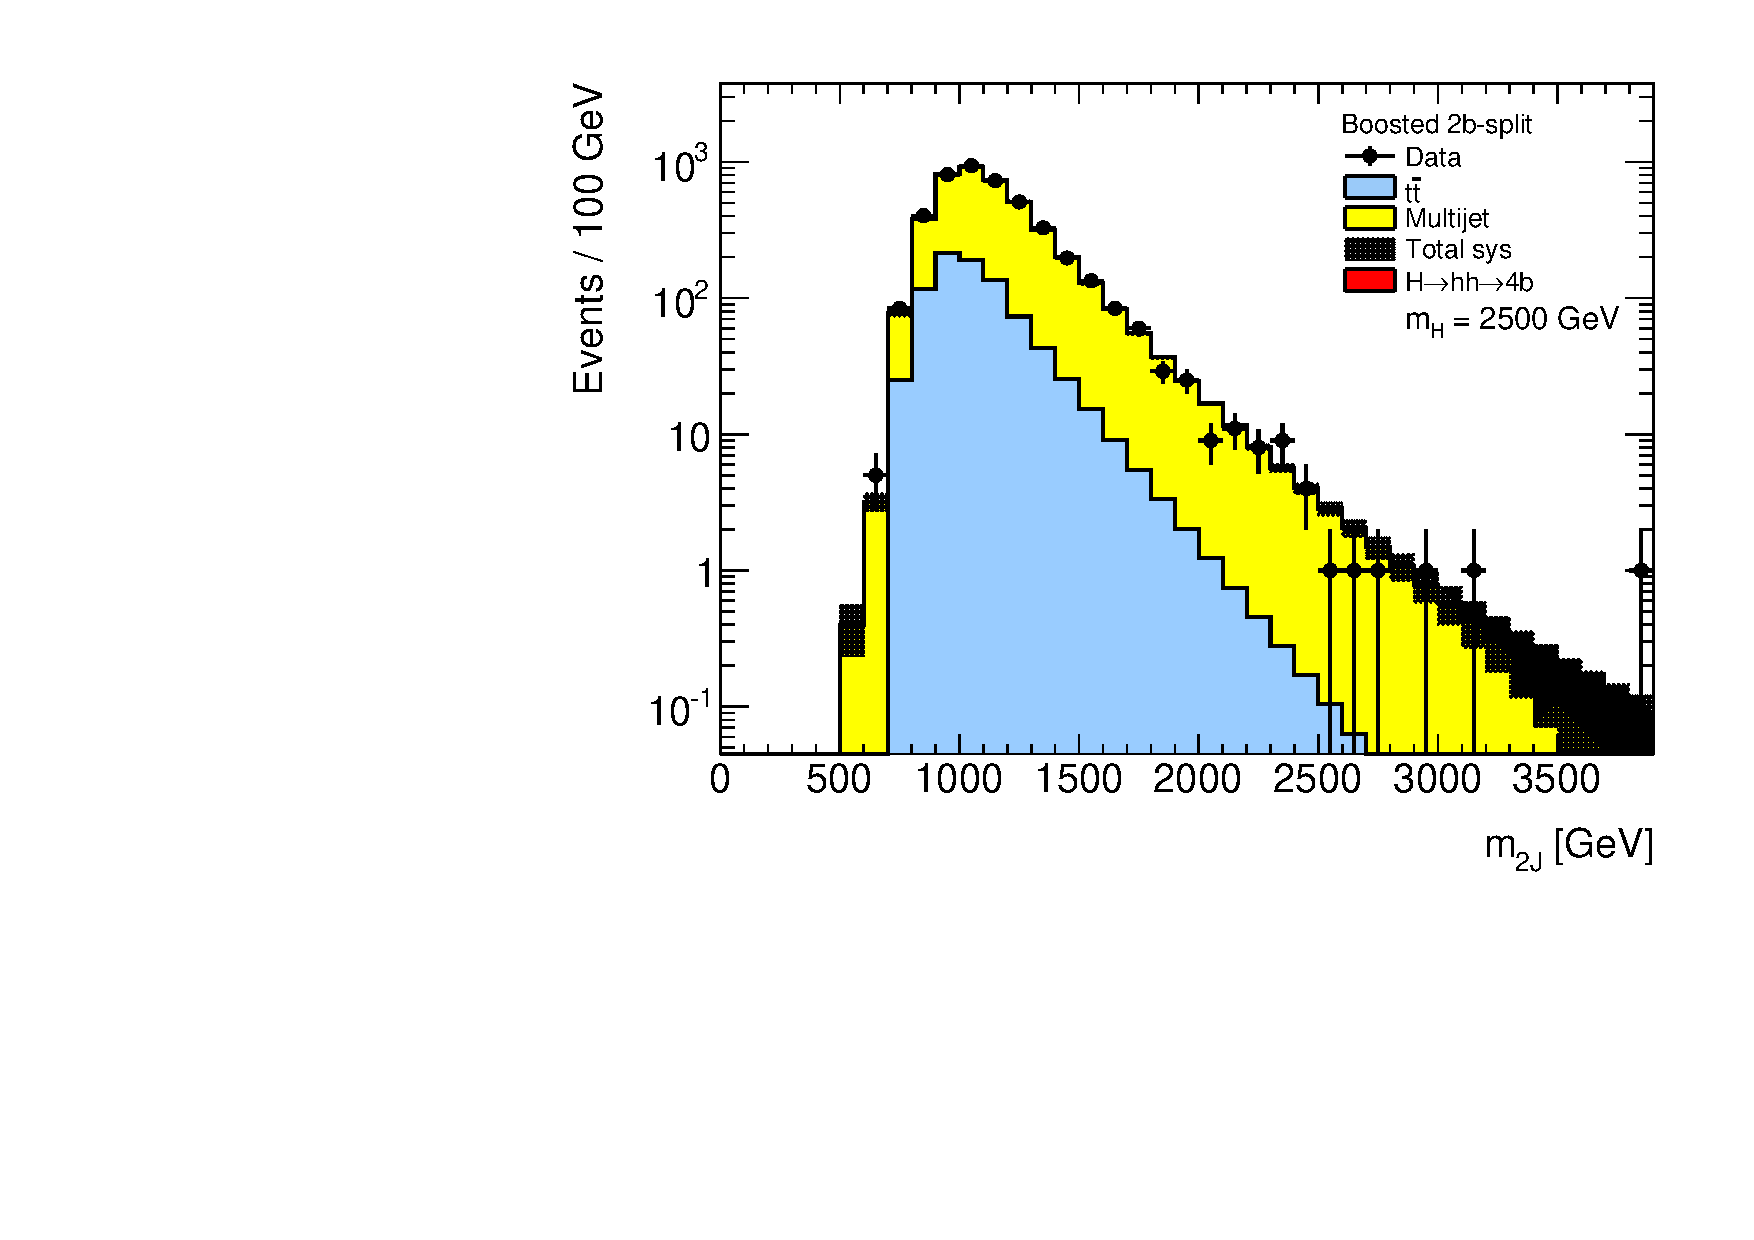
\includegraphics[width=0.21\textwidth,angle=-90]{figures/boosted/results/postfitplot_s_2500_b2b.pdf} 
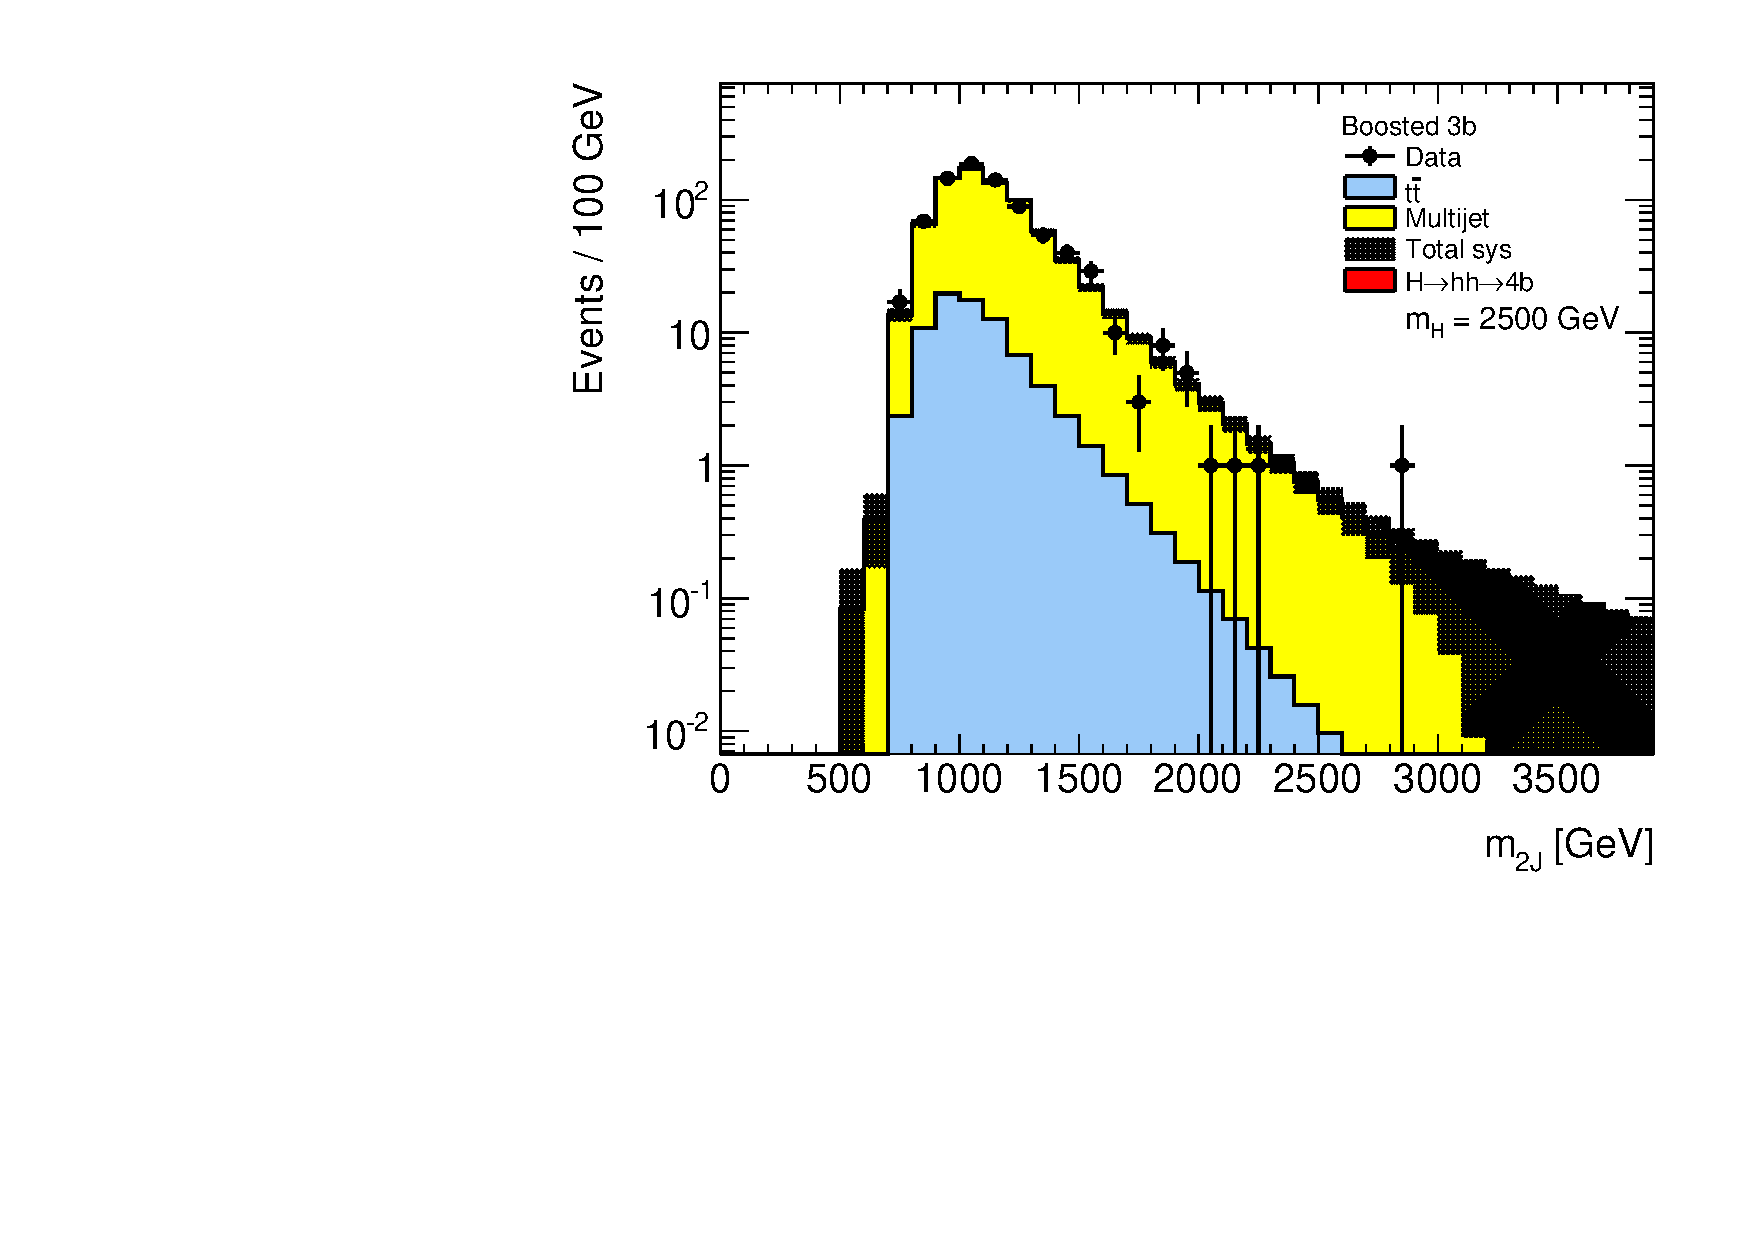
\includegraphics[width=0.21\textwidth,angle=-90]{figures/boosted/results/postfitplot_s_2500_b3b.pdf} 
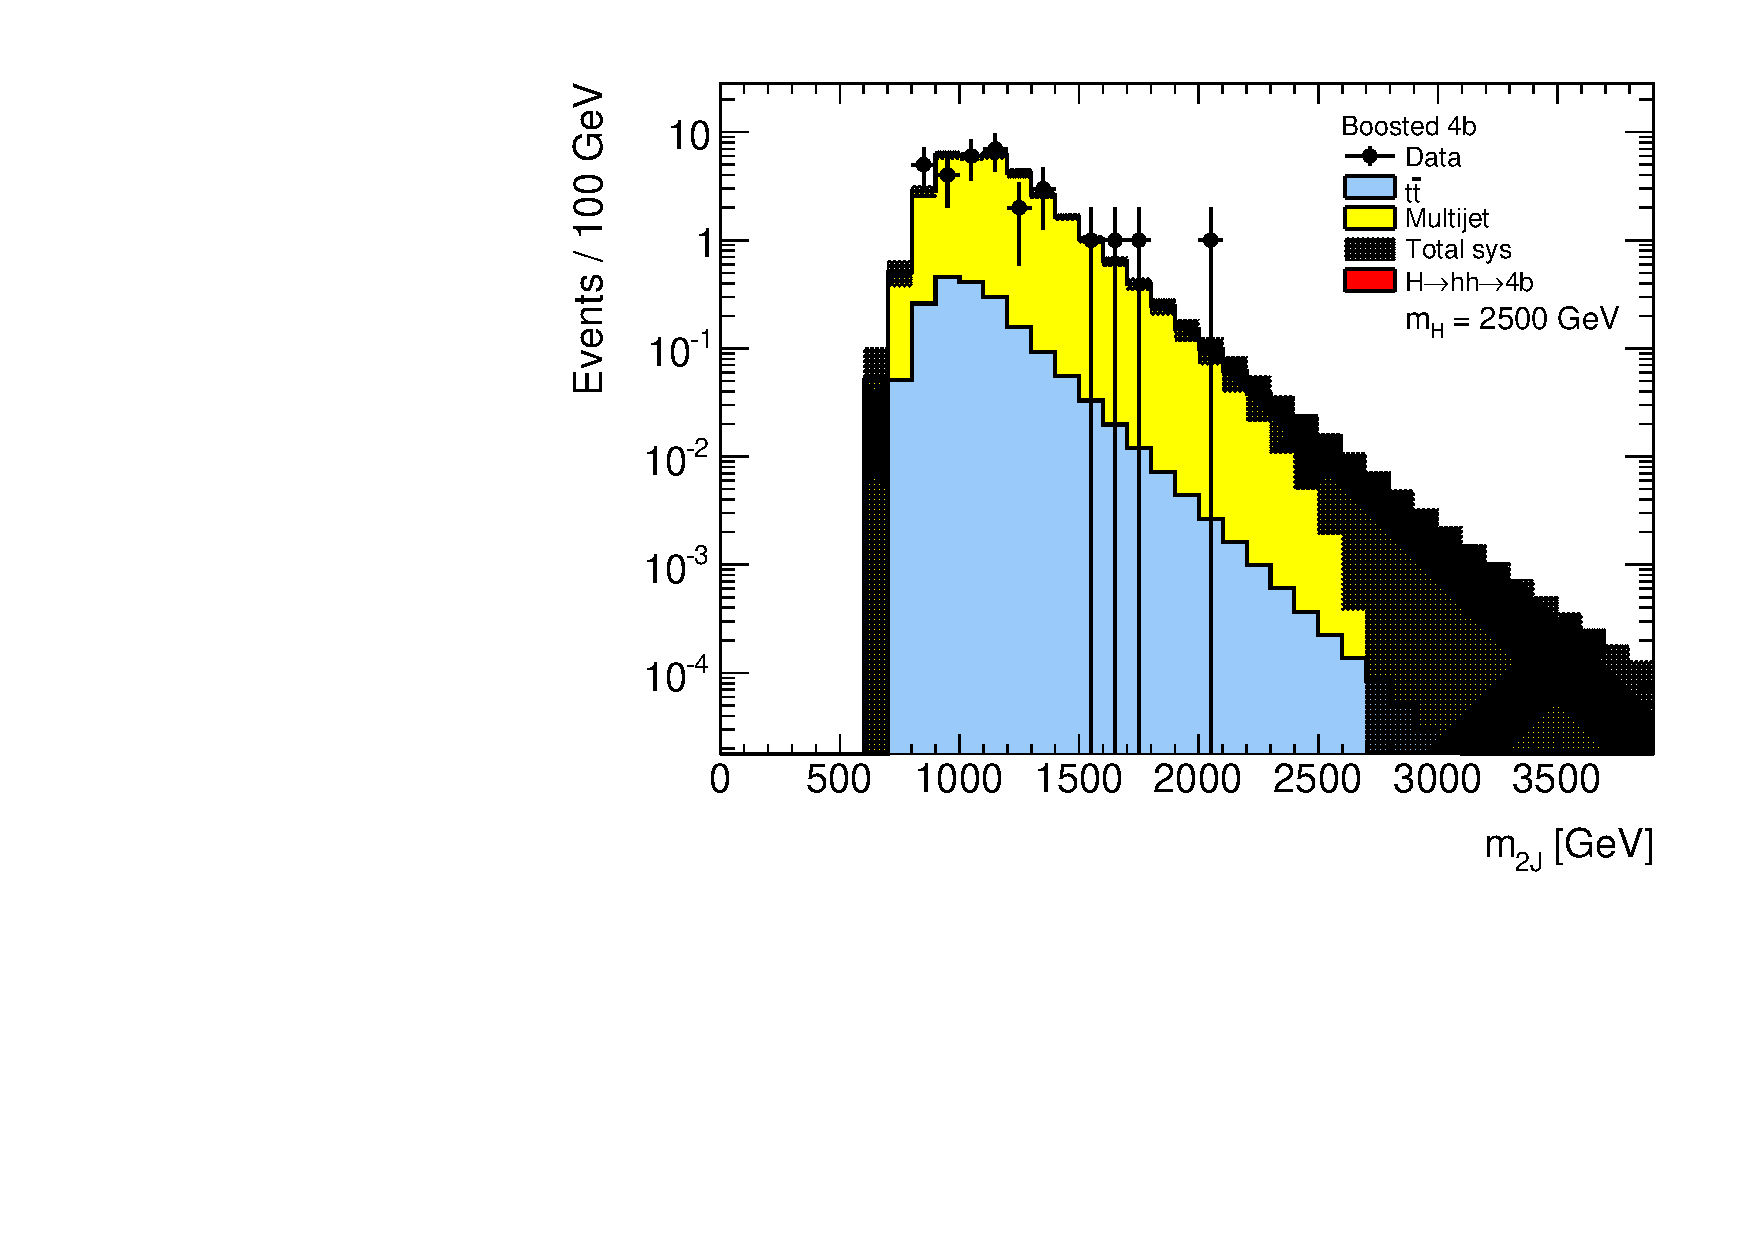
\includegraphics[width=0.21\textwidth,angle=-90]{figures/boosted/results/postfitplot_s_2500_b4b.pdf} 
\caption{Postfit distributions after fitting the data with the 2500 GeV signal hypothesis. The signal strength is zero.}
\label{fig:postfit2500}
\end{center}
\end{figure*}

The impact of the uncertainties on the fitted signal cross section is displayed in Fig.~\ref{fig:ranking2000} for the three signal models at 2000 GeV. The parameters are ranked by their postfit impact. Only the leading 30 nuisance parameters are displayed.

\begin{figure*}[htbp!]
\begin{center}
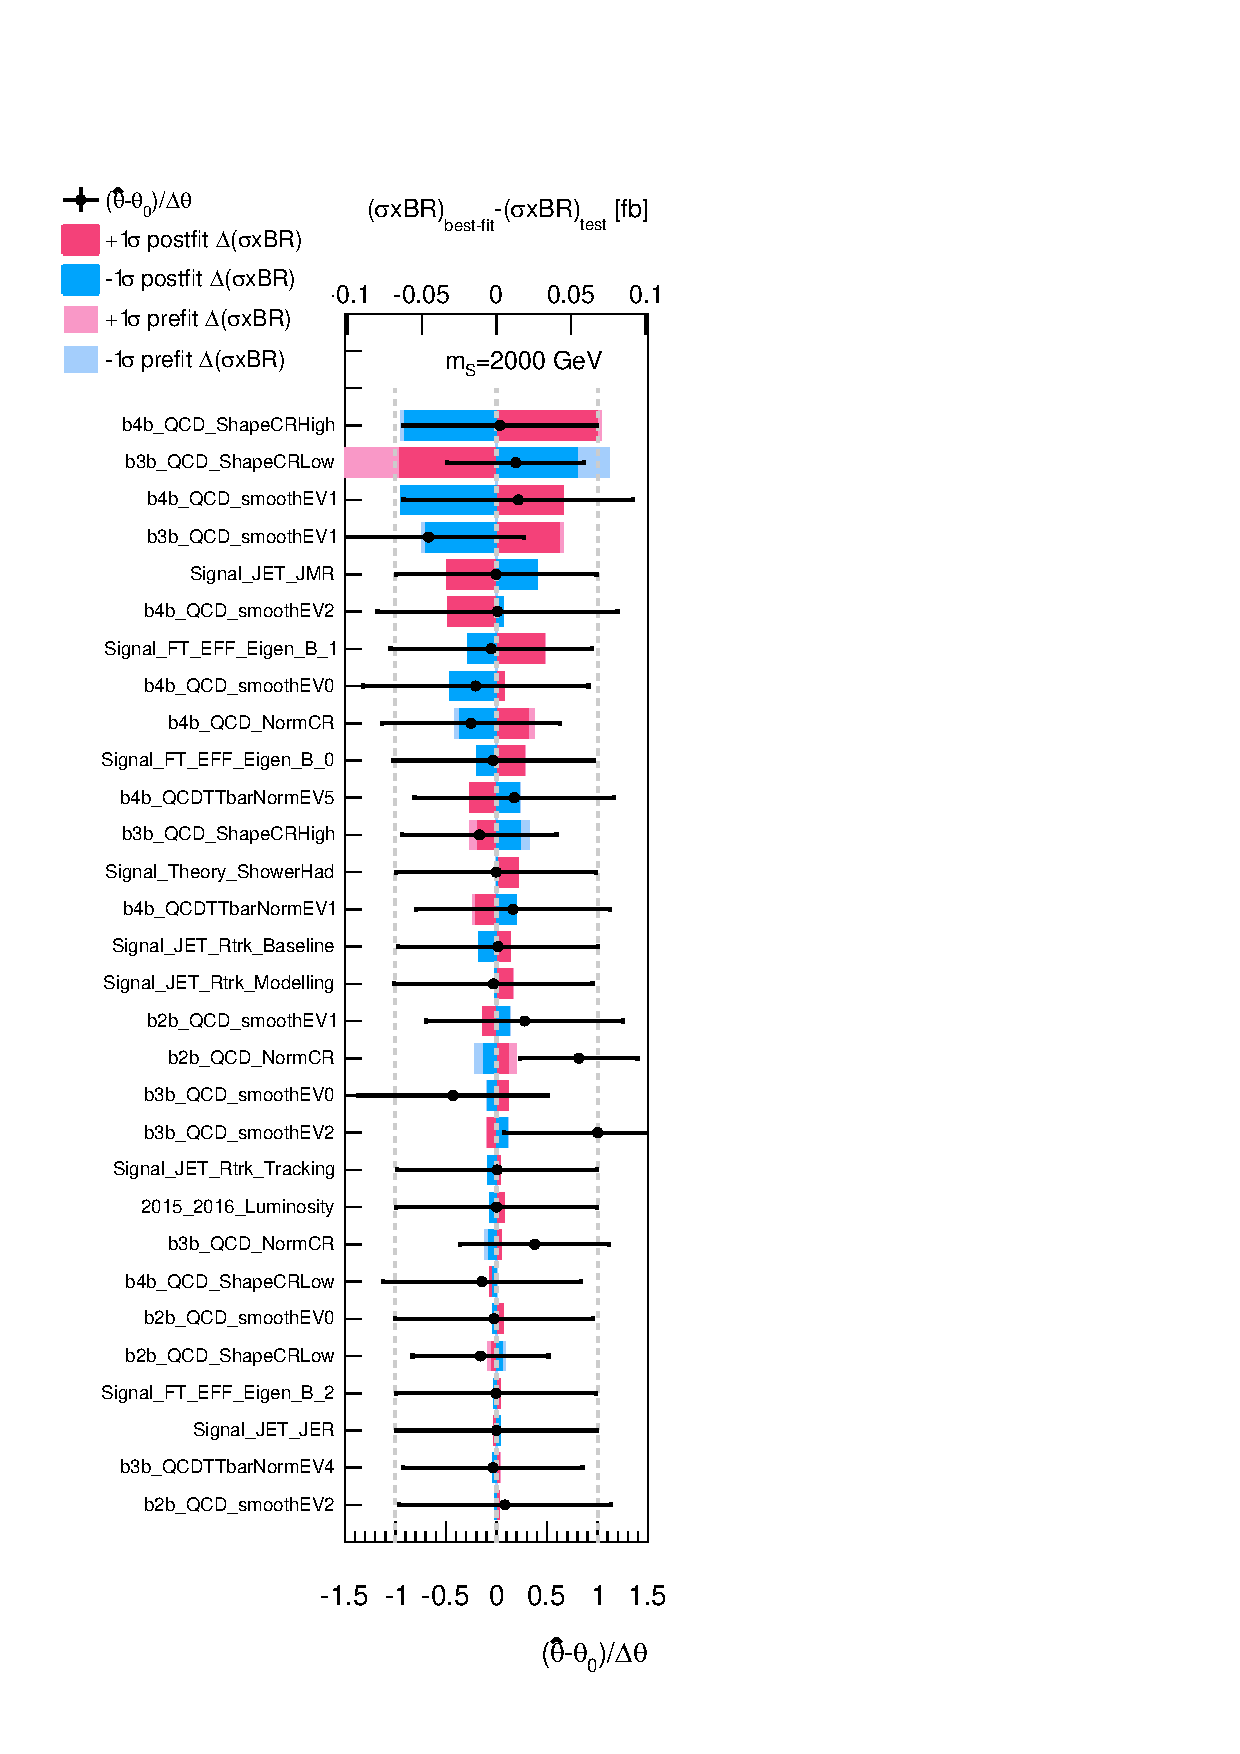
\includegraphics[width=0.21\textwidth]{figures/boosted/results/ranking_okt18_s_2000.pdf} 
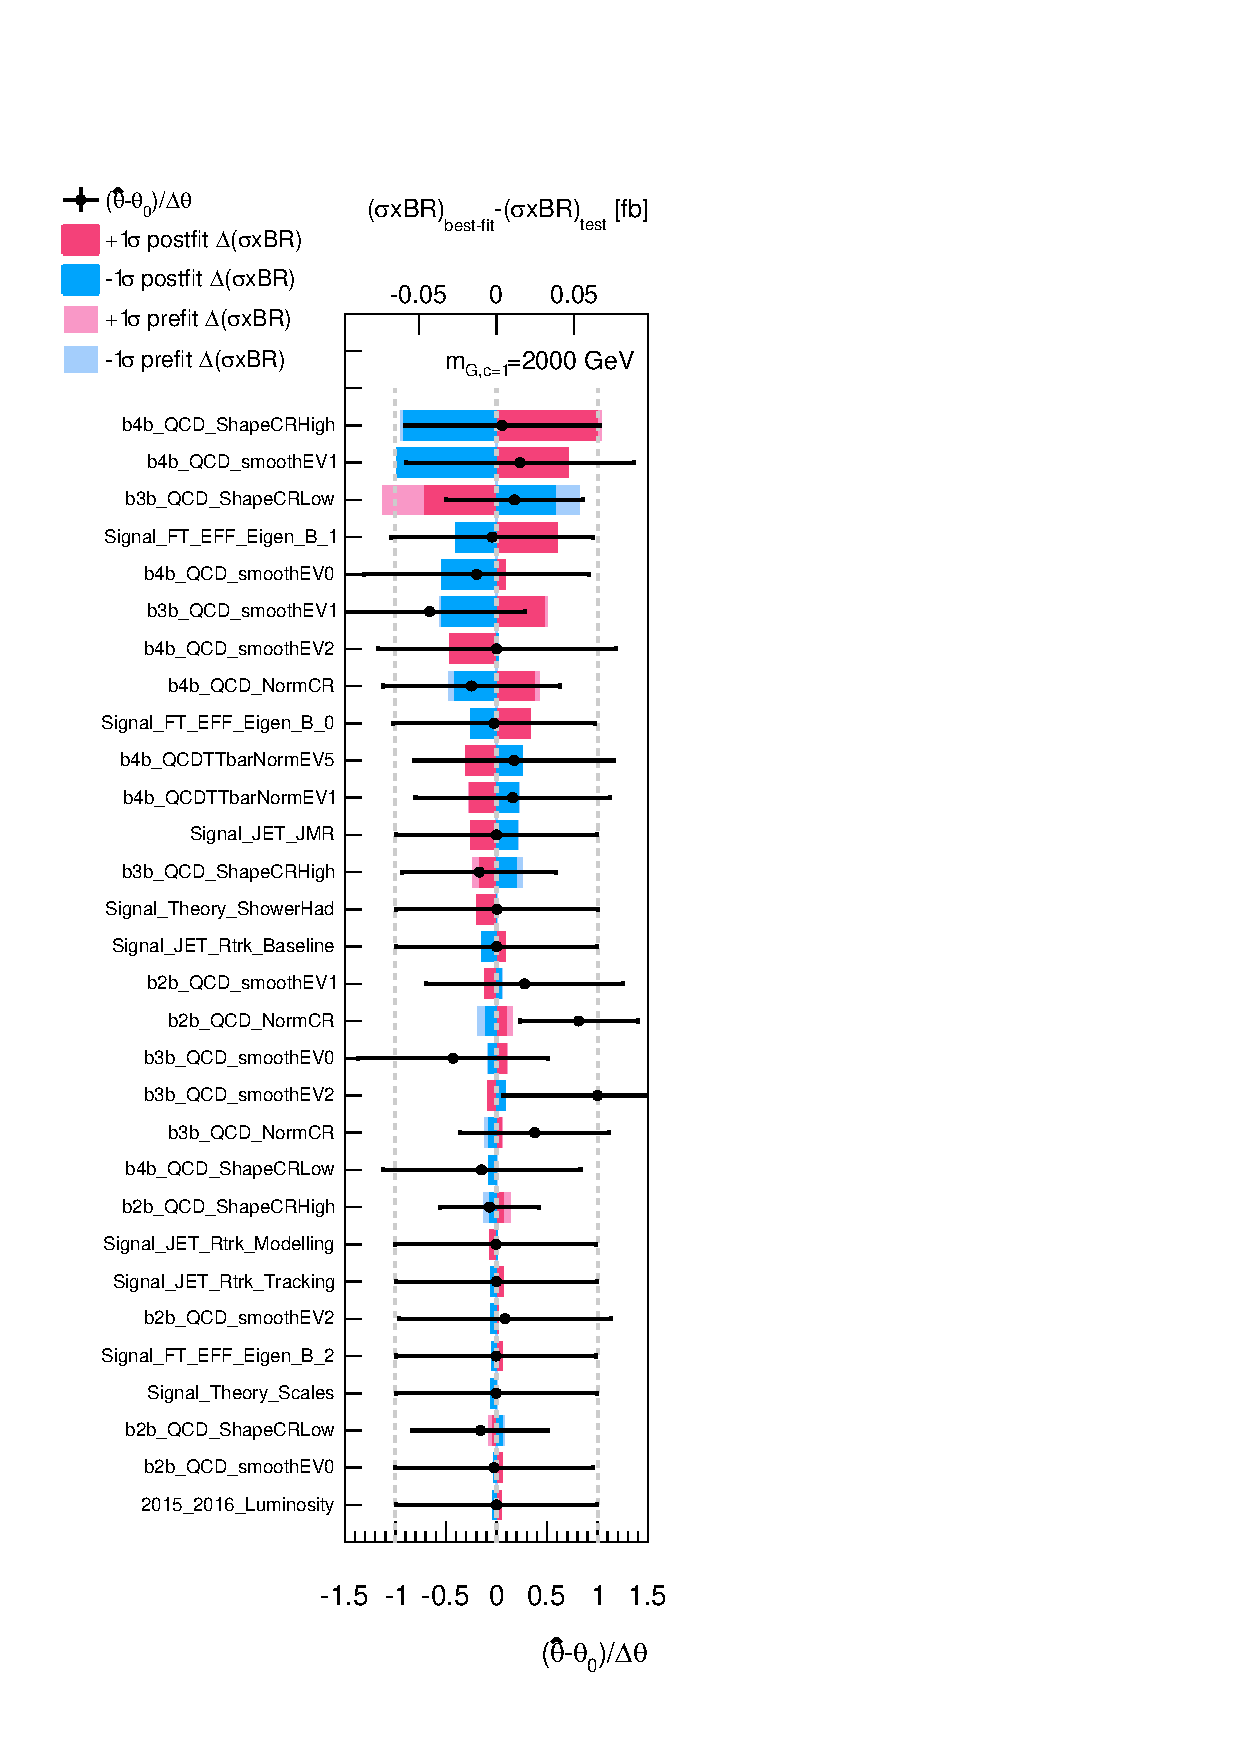
\includegraphics[width=0.21\textwidth]{figures/boosted/results/ranking_okt18_g10_2000.pdf} 
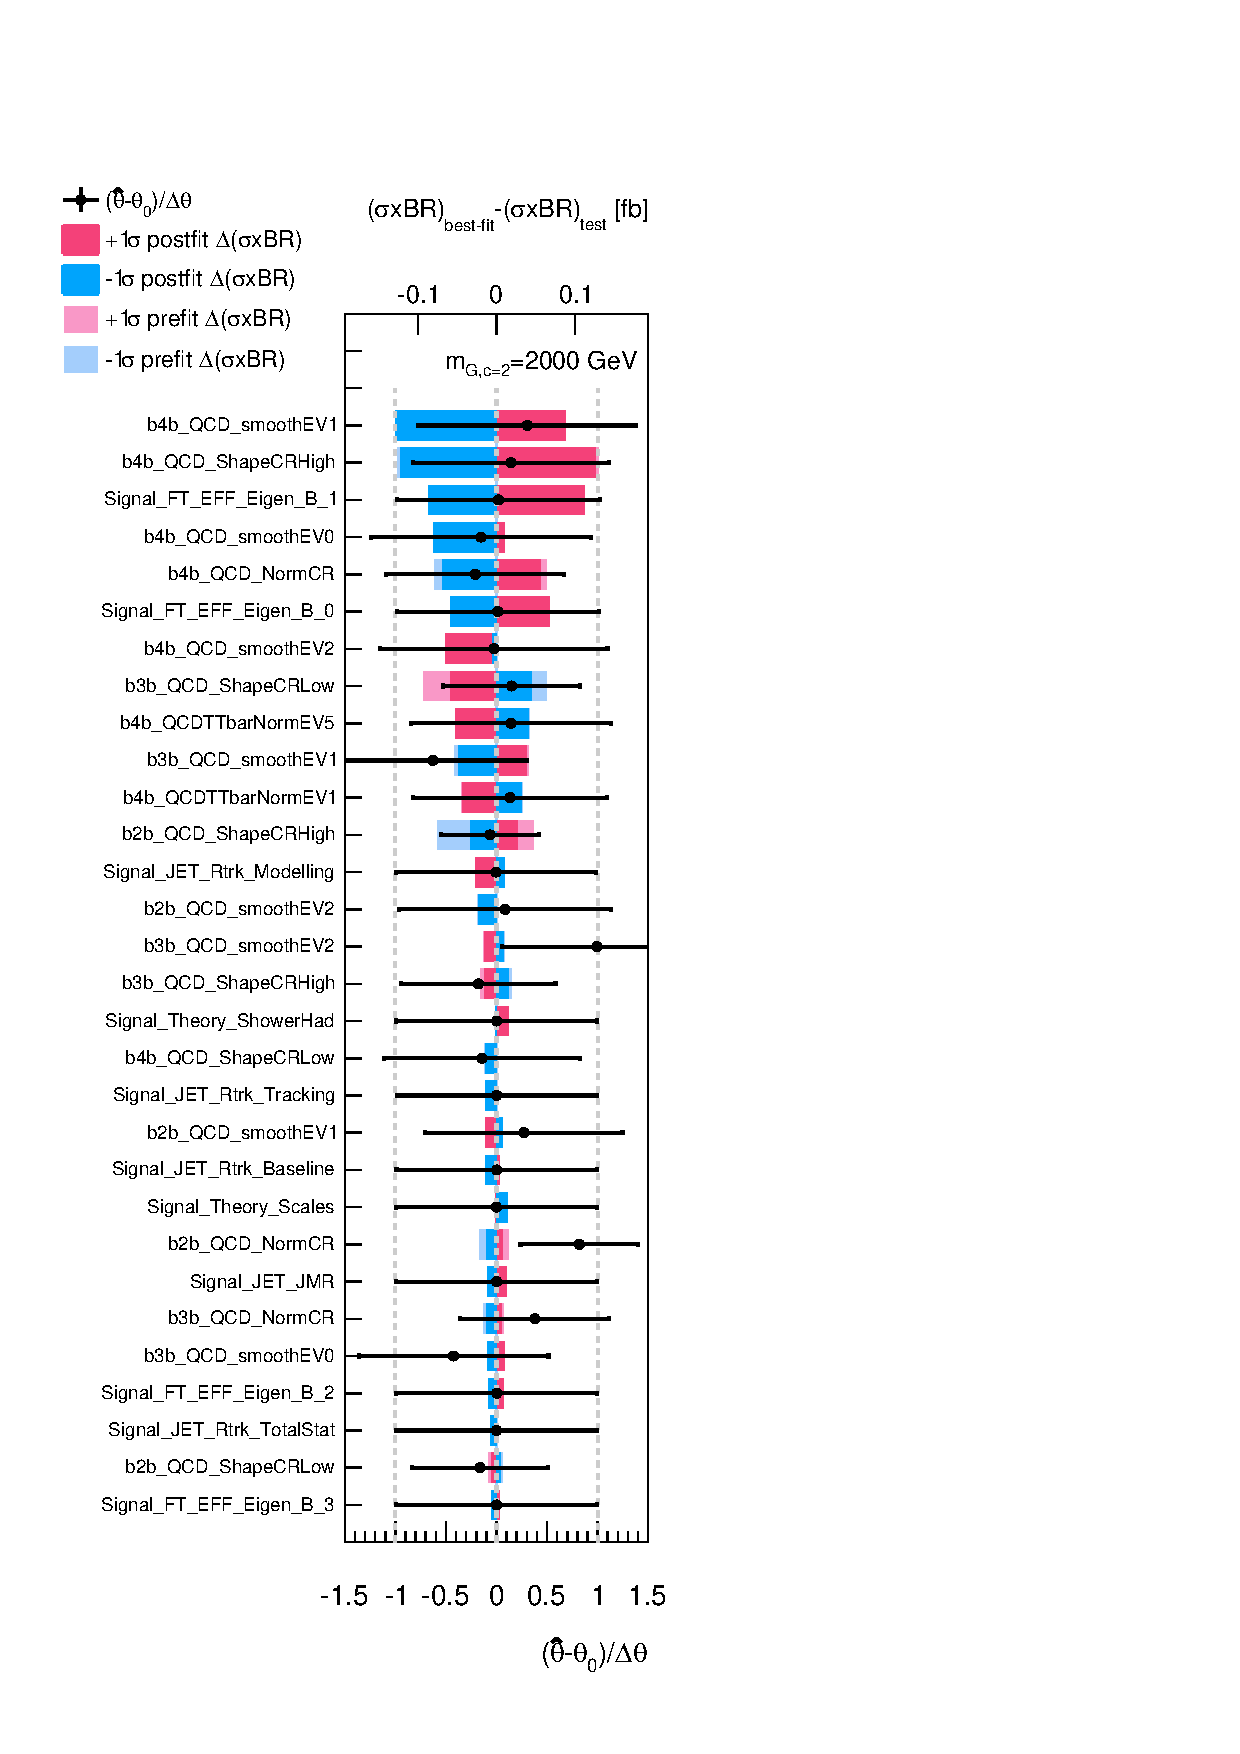
\includegraphics[width=0.21\textwidth]{figures/boosted/results/ranking_okt18_g20_2000.pdf} 
\caption{The impact of nuisance parameters on the fitted cross section, ranked by their postfit impact. The signal mass used in this fits is 2000~GeV, and the signal model is (a) narrow scalar, (b) c=1 Gravition and (c) c=2 Graviton.}
\label{fig:ranking2000}
\end{center}
\end{figure*}


